% Options for packages loaded elsewhere
\PassOptionsToPackage{unicode}{hyperref}
\PassOptionsToPackage{hyphens}{url}
%
\documentclass[
]{book}
\usepackage{lmodern}
\usepackage{amsmath}
\usepackage{ifxetex,ifluatex}
\ifnum 0\ifxetex 1\fi\ifluatex 1\fi=0 % if pdftex
  \usepackage[T1]{fontenc}
  \usepackage[utf8]{inputenc}
  \usepackage{textcomp} % provide euro and other symbols
  \usepackage{amssymb}
\else % if luatex or xetex
  \usepackage{unicode-math}
  \defaultfontfeatures{Scale=MatchLowercase}
  \defaultfontfeatures[\rmfamily]{Ligatures=TeX,Scale=1}
\fi
% Use upquote if available, for straight quotes in verbatim environments
\IfFileExists{upquote.sty}{\usepackage{upquote}}{}
\IfFileExists{microtype.sty}{% use microtype if available
  \usepackage[]{microtype}
  \UseMicrotypeSet[protrusion]{basicmath} % disable protrusion for tt fonts
}{}
\makeatletter
\@ifundefined{KOMAClassName}{% if non-KOMA class
  \IfFileExists{parskip.sty}{%
    \usepackage{parskip}
  }{% else
    \setlength{\parindent}{0pt}
    \setlength{\parskip}{6pt plus 2pt minus 1pt}}
}{% if KOMA class
  \KOMAoptions{parskip=half}}
\makeatother
\usepackage{xcolor}
\IfFileExists{xurl.sty}{\usepackage{xurl}}{} % add URL line breaks if available
\IfFileExists{bookmark.sty}{\usepackage{bookmark}}{\usepackage{hyperref}}
\hypersetup{
  pdftitle={YCHI5045M Statistics for Health Sciences: Computer Practical Session Notes},
  pdfauthor={Joe Hicks and Matt Mulvey},
  hidelinks,
  pdfcreator={LaTeX via pandoc}}
\urlstyle{same} % disable monospaced font for URLs
\usepackage{longtable,booktabs}
\usepackage{calc} % for calculating minipage widths
% Correct order of tables after \paragraph or \subparagraph
\usepackage{etoolbox}
\makeatletter
\patchcmd\longtable{\par}{\if@noskipsec\mbox{}\fi\par}{}{}
\makeatother
% Allow footnotes in longtable head/foot
\IfFileExists{footnotehyper.sty}{\usepackage{footnotehyper}}{\usepackage{footnote}}
\makesavenoteenv{longtable}
\usepackage{graphicx}
\makeatletter
\def\maxwidth{\ifdim\Gin@nat@width>\linewidth\linewidth\else\Gin@nat@width\fi}
\def\maxheight{\ifdim\Gin@nat@height>\textheight\textheight\else\Gin@nat@height\fi}
\makeatother
% Scale images if necessary, so that they will not overflow the page
% margins by default, and it is still possible to overwrite the defaults
% using explicit options in \includegraphics[width, height, ...]{}
\setkeys{Gin}{width=\maxwidth,height=\maxheight,keepaspectratio}
% Set default figure placement to htbp
\makeatletter
\def\fps@figure{htbp}
\makeatother
\setlength{\emergencystretch}{3em} % prevent overfull lines
\providecommand{\tightlist}{%
  \setlength{\itemsep}{0pt}\setlength{\parskip}{0pt}}
\setcounter{secnumdepth}{5}
\usepackage{booktabs}
\usepackage{longtable}
\usepackage{array}
\usepackage{multirow}
\usepackage{wrapfig}
\usepackage{float}
\usepackage{colortbl}
\usepackage{pdflscape}
\usepackage{tabu}
\usepackage{threeparttable}
\usepackage{threeparttablex}
\usepackage[normalem]{ulem}
\usepackage{makecell}
\usepackage{xcolor}
\ifluatex
  \usepackage{selnolig}  % disable illegal ligatures
\fi
\usepackage[]{natbib}
\bibliographystyle{apalike}

\title{YCHI5045M Statistics for Health Sciences: Computer Practical Session Notes}
\author{Joe Hicks and Matt Mulvey}
\date{International Health MSc (2021)}

\begin{document}
\maketitle

{
\setcounter{tocdepth}{1}
\tableofcontents
}
\begin{verbatim}
## 
## Attaching package: 'xfun'
\end{verbatim}

\begin{verbatim}
## The following objects are masked from 'package:base':
## 
##     attr, isFALSE
\end{verbatim}

\begin{verbatim}
## 
## Attaching package: 'downloadthis'
\end{verbatim}

\begin{verbatim}
## The following object is masked from 'package:xfun':
## 
##     download_file
\end{verbatim}

\hypertarget{aims-and-objectives}{%
\chapter{Aims and objectives}\label{aims-and-objectives}}

The aim of these YCHI5045M Statistics for Health Sciences computer practical sessions is to help you develop skills and experience in carrying out the main statistical steps required to conduct a quantitative research study.

The key objectives for these sessions are for you to gain skills and experience in:

\begin{enumerate}
\def\labelenumi{\arabic{enumi}.}
\item
  Calculating sample sizes applicable to common study designs.
\item
  Taking statistically representative ``probability samples'' from sampling frames using a range of common methods.
\item
  Preparing ``raw'' unprocessed data for analysis.
\item
  Exploring, describing and visualising sample data.
\item
  Using a small but powerful range of classical ``statistical tests'' and more modern ``statistical models'' to make inferences (generalisations) about hypothesised causal relationships in data in order to answer research questions.
\item
  Correctly and meaningfully interpreting the results of these statistical analyses in terms of their implications for research questions and hypotheses.
\end{enumerate}

We will cover these aims in turn and most of our time will be spent on objectives 5 and 6. To calculate sample sizes we will use a user-friendly, web-based, sample size calculator, and to sample from a sampling frame we will use Microsoft Excel. While to prepare, edit, and analyse data we will use a commonly used statistical software package called SPSS.

\hypertarget{statistical-paradigm}{%
\section{Statistical paradigm}\label{statistical-paradigm}}

As with the lectures in these practical sessions we will only look at statistical methods that take a ``frequentist'' approach (or use a ``frequentist paradigm'') to statistical inference: \url{https://en.wikipedia.org/wiki/Frequentist_inference}

\hypertarget{analyses-covered}{%
\section{Analyses covered}\label{analyses-covered}}

There are many, many methods for analysing data to draw statistical inferences, but in these sessions we will only cover a selection of the most commonly used/seen. These include some of the ``classical statistical tests'' like the independent t-test and the chi-squared test of independence, as well as two common types of regression models: linear regression and logistic regression. We primarily include the statistical tests so you can become familiar with using them if you wish, but our recommendation is not to focus on them but to become comfortable and competent at using the two regression modelling approaches covered, and if you were to go further in your learning to explore additional modelling approaches like Poission regression, negative binomial regression, and/or multi-level regression models.

We recommend this for two main reasons. First, broadly speaking any analysis you can do using a classical statistical test can be replicated using a regression model, and all of the analyses using the statistical tests we cover here can be replicated (broadly speaking) using linear or logistic regression. Second, not only can regression models replicate the analyses done using classical statistical tests, but they offer the substantial advantage that you can also adjust for any number and type of ``confounding variables'' and/or ``competing exposures'' when estimating your relationships of interest. Given that it's probably fair to say that no dataset is free of these issues, particularly any observational dataset, why use an analysis that is by definition not able to help you adjust for them and thereby obtain more biased results? Additionally, some classical statistical tests like the chi-squared test of independence don't even allow you to estimate confidence intervals around your estimate of your relationship of interest, just a p-value, and as we'll repeatedly state the key inferential statistic of interest should be your estimate of your relationship of interest and the confidence intervals around it.

\hypertarget{preliminary-information}{%
\chapter{Preliminary information}\label{preliminary-information}}

\hypertarget{datasets-and-exercises-document}{%
\section{Datasets and exercises document}\label{datasets-and-exercises-document}}

Before going any further please download the datasets that we will be analysing later on and the exercises document that you will use to complete some of the exercises. All these files can be downloaded as a ``zip'' file by clicking on the button below.

Download YCHI5045M computer practical files

A zip file is a compressed file, or in this case a set of files within folders, which you can ``unzip'' or extract and then view/open the files in the folders. If you don't know how to unzip the file on Windows or can't unzip it for some reason you can download the free Winrar unzipping software from:

www.win-rar.com

And Mac users should be able to unzip zip files with the in-built MacOS unzipping software.

When you unzip the file and go into the you should see two folders: ``Datasets'' and ``Exercises''. All the datasets you will use are within the ``Datasets'' folder, and within the ``Exercises'' folder is a Word document called ``Exercises.docx'' that you will use when completing some of the exercises.

\hypertarget{a-word-of-encouragement}{%
\section{A word of encouragement}\label{a-word-of-encouragement}}

(If you want/need it!)

Students often find learning and doing statistics to be hard, sometimes very hard! Unfortunately this is to be expected and there are no short-cuts or secrets. Unless you are a genius then like most people, including ourselves, to really begin to understand statistics more deeply and to be able to confidently and correctly analyse typical datasets independently will take a lot of time and effort. However, we firmly believe that it is perfectly possible for any motivated student to get to any level of skill and understanding they wish to reach if they are simply prepared to put in the necessary effort and practice, and the rewards can be huge. Being able to correctly run and interpret even simple statistical analyses gives you skills that are highly valuable in the world of research, and which are increasingly valuable and sought after in the wider world. So please don't despair when things seem difficult or impossible. We've all felt that way, but like any new skill it really does gets easier and easier with practice, and it can even be enjoyable (no really, being able to take a dataset and generate insights about the world can be a really exciting and enjoyable process!).

\hypertarget{about-these-notes}{%
\section{About these notes}\label{about-these-notes}}

These notes are intended to serve as both a comprehensive guide to the introductory statistics computer practical sessions we will be doing and, if you wish, as a longer-term reference document for when you are analysing data. In particular, you can refer to this document for guidance on your statistical analyses when you are completing the summative assessment for this module, and for your data collection and data analysis planning and activities during your dissertations/research projects, if they involve any quantitative analyses.

The aim of these notes is not just to explain how to do the methods covered but also to discuss how to apply them to real-world studies and how to understand and interpret the results. We also aim to show you how to try and deal with some of the most common challenges faced when planning studies or working with real-world data. You may therefore feel the notes contain too much detail but actually we feel they really only cover the basics. However, we have tried to limit the display of information that you may not wish or need to view right away when simply learning how to use the methods covered by using buttons that can reveal or re-hide such information.

For all key software processes (like running analyses) we provide step-by-step video-based and text-based instructions that are largely identical, and so you can choose whether to watch a video or read some text to understand how to do everything. Therefore, there is no need to view both sets of instructions, although you may find the videos helpful at first to see what to do in the software and then refer to relevant parts of the text instructions later on for a quick reminder as necessary.

Note: with the text instructions we refer to menus, tools, options (like tick boxes) and buttons etc in the different pieces of software using highlighted text like this.

\textbf{Please note that all SPSS instructions relate to SPSS version 27, which is the version that I have on my computer. This may not be the version that you are using either on a campus computer or your own computer. However, SPSS typically changes very little from version to version, especially when it comes to standard tools and analyses. So although things may look a little different for you there shouldn't (hopefully) be any issues in following the instructions.}

\hypertarget{how-these-sessions-relate-to-the-summative-assignment}{%
\section{How these sessions relate to the summative assignment}\label{how-these-sessions-relate-to-the-summative-assignment}}

In summary: we do not expect you to use any methods other than those that we will cover in these sessions when analysing data for the summative assignment.

Full details:

Please see the ``YCHI5045M 20-21 Assignment Guidance.doc'' document for full guidance on the summative assignment. This can be downloaded from Minerva. From the YCHI5045M module page under the \emph{Assessment and Feedback} heading go to the \emph{Assessment} page and look for the \emph{Assignment Information} section.

However, in summary: for the summative assignment you will need to analyse a dataset on your own. Don't panic! The analysis methods explained in this handout are completely sufficient to analyse the dataset provided for the summative assignment, and \textbf{we do not expect you to use any other methods than those taught in these sessions} for your summative assignment analyses. You can certainly use any other methods you already know, or subsequently learn if you wish. However, it is of course your responsibility to ensure you use them correctly and, just as importantly, to demonstrate that you have used them correctly by providing evidence that all relevant assumptions were met etc, otherwise you will fail to gain full marks.

Based on the methods/analyses you will learn in these sessions, it is up to you to decide which are most suitable for your summative assignment analyses given the research question and data provided in the summative assignment. Some methods may be simply less robust choices, and therefore produce results which may be accurate but will be more prone to bias, while other methods will not make sense (or even work) given the data and research question. Hopefully this should be clear though after these sessions.

There is therefore some flexibility in which methods you can use and you can certainly use any suitable methods, and you should consider the trade-off between using a more robust method vs a less robust method which you may be more comfortable with and less likely to make a mistake with. However, to gain the highest mark with whatever methods you use you must demonstrate a clear awareness of the limitations and risks of bias associated with those methods. This is particularly important if you choose to use simpler methods of analysis (e.g.~t-tests instead of multiple linear regression).

\hypertarget{about-this-website}{%
\section{About this website}\label{about-this-website}}

You can change the font options using the button at the top of the website (the capital letter ``A''). This lets you do things like use a dark theme that is easier on your eyes than staring at a bright white screen all day, change the font, and change the size of font. There is also a search button, you can navigate between pages using the left and right arrow keys, and lastly you can hide the menu by clicking on the left-most button on the top menu.

\hypertarget{probability-sampling}{%
\chapter{Probability sampling}\label{probability-sampling}}

\hypertarget{units-of-observation-and-analysis}{%
\section{Units of observation and analysis}\label{units-of-observation-and-analysis}}

Two key terms/definitions to understand before we go further are:

\begin{itemize}
\item
  Unit of observation: the entities (e.g.~people, health facilities) that are described by the data, or more practically speaking the entities that you collect data from. The unit of observation should be further definable in terms of the range of characteristics that the entities have (e.g.~the eligibility criteria of the study), and in terms of the spatial and temporal parameters of the study and data collection process (e.g.~patients visiting any of the study health facilities between January 1st 2020 to January 1st 2021, including multiple visits).
\item
  Unit of analysis: the entities that you are analysing in your study and aiming to make statistical inferences about using the data collected. The unit of analysis is therefore defined both by how you collect your data but also by how you analyse it.
\end{itemize}

\begin{quote}
Often the unit of observation and analysis will be the same. For example, in most typical cross-sectional surveys the individual will be both the unit of observation and analysis. However, this won't always be the case. For example, in a cluster randomised controlled trial you may collect data from individual patients but their outcomes might be aggregated at the cluster-level (e.g.~binary patient-level outcomes converted to cluster-level proportions) and then compared between treatement arms, in which case the unit of observation would be the patient but the unit of analysis would be the cluster (e.g.~the health facility).
\end{quote}

\hypertarget{overview}{%
\section{Overview}\label{overview}}

Broadly speaking ampling is the process whereby we choose which units of observation or ``sampling units'' within our target population we will collect data from. \emph{Therefore, the first stage of sampling, which should always occur very early on in the research and study design process, is when you clearly and explicitly define your target population}. In summary, the only sampling methods that are guaranteed to produce unbiased statistical inferences, albeit only on average or ``in the long-run'', are ``probability sampling'' methods. This is because all standard statistical methods of analysis assume that sample data are randomly sampled from a given target population using some specific form of probability sampling. Therefore, the only way to robustly satisfy this assumption is clearly to take some form of probability sample.

To take a probability sample you require a sampling frame, which is just a list of all units of observation in the target population that you are aiming to generalise your results to (e.g.~all individuals in a region, all primary care health facilities in a country etc). \emph{Therefore, the second stage of any sampling process is to obtain or create a sampling frame for your target population}. Note: for a probability sampling method to be valid it must be possible, at least in theory although you wouldn't actually do it in practice, to calculate each unit of observation's probability of being selected, which may or may not be equal for all units, and should not be zero for any unit.

For most sampling methods we require a complete and comprehensive sampling frame before we actually sample. Although for some multi-stage sampling approaches, including those typically used by large-scale household surveys (as discussed in the lecture), you can use incomplete sampling frames to start your sampling and construct additional but still incomplete sampling frame(s) during your sampling process to achieve a robust probability sample. However, as these multi-stage approaches are quite complicated and you would not be advised to undertake them without extensive statistical support we will not practice them here.

In these sampling practical sessions we will therefore look at how you can apply most of the commonly used simple probability sampling methods, specifically simple random sampling, a stratified random sampling with \emph{proportionate stratification} and \emph{disproportionate stratification}, and systematic random sampling. We will assume we have a complete sampling frame for our hypothetical target population. We will also note how these methods can also be used to take single-stage cluster samples with complete second/final-stage sampling, and how they can be combined into multi-stage cluster samples. However, we will not actually practice these much more complicated methods as it's very unlikely you would ever need to implement them yourself (unless you become a survey methodologist etc).

\hypertarget{non-probability-sampling}{%
\section{Non-probability sampling}\label{non-probability-sampling}}

While desirable it is clearly often not feasible to use probability sampling methods, usually because of the lack of a suitable sampling frame. For example, if you are studying patients attending a healthcare facility over a given period and you need to collect data on sampled patients \emph{on the day they attend the facility} it's typically impossible to construct a sampling frame because you won't know who will be visiting each day! Therefore, you may often need to resort to non-probability sampling methods such as quota sampling or convenience sampling, and just try to make your samples as representative of your target population as you can, while minimising the opportunity for any researcher sampling bias.

Broadly speaking it is often more justifiable to generalise results from analytical (associational) studies that use non-probability sampling methods than from descriptive studies (surveys) that use non-probability sampling methods, and consequently if you are aiming to describe certain characteristics of a given target population you should aim to take a probability sample. However, you may often be able to make a good justification that results from an analytical study can be generalised despite the study using non-probability sampling methods. For example, many (maybe most) trials of patient-level treatments use non-probability samples, often convenience samples taken at health facilities as patients attend, due to the difficulty of taking a true probability sample. In such circumstances it is often justifiable to generalise the results to other individuals who share similar key characteristics with the trial sample (e.g.~age, sex, and biomedical characteristics distributions), because patient-level treatments often work fairly similarly across different populations with similar characteristics. This may be much less justified for complex interventions delivered at higher levels, such as complex interventions with staff-level and facility-level components, because the effects of these types of interventions are likely to be much more dependent on the study's context. Hence, generalising the results of complex interventions from studies like cluster trials that use non-probability samples may be much more questionable. The only ``solution'' is to think very carefully when planning your sampling methods and think explicitly from the start about who you want your results to robustly generalise to.

\hypertarget{simple-random-sampling}{%
\section{Simple random sampling}\label{simple-random-sampling}}

\hypertarget{overview-1}{%
\subsection{Overview}\label{overview-1}}

Simple random sampling involves taking a random sample of a given size from a sampling frame, which results in each unit of observation having an equal probability of being selected. You can take a simple random sample from a sampling frame in various ways, such as by generating random numbers that correspond to IDs that are pre-allocated to all units of observation, or you can do it by simply randomly sorting the list and just selecting the first n units of observation, where n is your sample size. We will use this second approach as it's easy to implement in Excel.

\hypertarget{advantages-of-simple-random-sampling}{%
\subsection{Advantages of simple random sampling}\label{advantages-of-simple-random-sampling}}

\begin{itemize}
\item
  Easy to implement and explain.
\item
  Requires minimal data on your target population units of observation: just a list of all units of observation, plus usually some way of identifying/contacting them once selected.
\end{itemize}

\hypertarget{disadvantageslimitations-of-simple-random-sampling}{%
\subsection{Disadvantages/limitations of simple random sampling}\label{disadvantageslimitations-of-simple-random-sampling}}

\begin{itemize}
\item
  Although simple random sampling guarantees that you will select a sample that is representative (i.e.~unbiased) of your target population \emph{on average/in the long-run}, i.e.~over many hypothetically repeated samples, it is not the best approach at achieving this goal for any given sample, and obviously in practice you typically only ever take one sample! This is especially the case when the population is heterogeneous (highly varied in the characteristics/relationships of interest) and/or if sample size is small, say in the tens or low hundreds rather than the high hundreds or thousands (as the sample size increases the chances of getting an unrepresentative sample decrease). As these two situations are often true it is often better to use stratified random sampling instead, if possible.
\item
  If your sampling units cover a large geographical area simple random sampling can produce a very logistically inefficient, costly, and geographically spread-out sample. See cluster sampling for an possible solution to this problem.
\end{itemize}

\hypertarget{scenario}{%
\subsection{Scenario}\label{scenario}}

You work for a district governmental health department and you have been tasked with assessing the capacity and service delivery characteristics of the public primary care facilities within your district. Specifically, you need to report the typical (e.g.~mean/median) staffing levels (e.g.~the no. drs and nurses), resources and equipment levels (e.g.~no. beds, no. oxygen canisters, no. x-ray machines), and services delivery levels (e.g.~the no. of deliveries with a skilled birth attendant during the last 6 months, the no. of under 5s receiving their full set of vaccinations during the last 6 months etc) for all public primary care facilities.

However, while there are 246 such facilities within your district you only have resources to survey 50 facilities (if you could survey all 246 it would be a ``census'' not a sample). A sample size calculation indicates that this will be sufficient to provide usefully precise estimates of these characteristics, but your results need to be robustly generalisable to the district, i.e.~your target population is all public primary care facilities within your district.

Luckily there is an existing comprehensive list (i.e.~sampling frame) of all 246 existing public primary care facilities in your district. You have a copy of this list, in the form of an Excel spreadsheet, that includes facility names, addresses and telephone numbers, plus additional information that we will use in subsequent exercises.

Our aim is therefore to take a simple random sample of 50 facilities from the list.

\hypertarget{exercise-taking-a-simple-random-sample-using-excel}{%
\subsection{Exercise: taking a simple random sample using Excel}\label{exercise-taking-a-simple-random-sample-using-excel}}

\begin{itemize}
\tightlist
\item
  Load the ``Health facilities list - simple random sample.xlsx'' Excel spreadsheet.
\end{itemize}

\href{https://youtu.be/GrHFm7VlNt4}{Video instructions: taking a simple random sample using Excel}

\textbf{Written instructions: taking a simple random sample using Excel}

\begin{itemize}
\item
  In the ``Health facilities list - simple random sample.xlsx'' Excel spreadsheet you will see it has various self-explanatory columns/variables including ``facility\_name'', ``facility\_address'', and ``facility\_tel''.
\item
  In column A (the blank column immediately to the left of the ``facility\_name'' column) enter the following (or similar) word as a heading: random\_no
\item
  Immediately under this new column in cell A2 (the first row where the facility data starts) click on the cell and type =rand() and press enter. This Excel function generates a random number between 0 and 1 to six decimal places.
\item
  Then simply ensure that cell A2 is selected (i.e.~you've clicked on it) and then just double click on the small solid square at the very bottom right of this cell. This should copy and paste the function all the way down to the end of the facility data.
\item
  Next click on the ``random\_no'' column heading (cell A1) and then in the menu ``ribbon'' click on Data and click the Filter tool. You should see little ``drop-down'' menu buttons appear in the right of each column heading. Click on the drop-down menu button in the ``random\_no'' column heading (cell A1) and select Sort Smallest to Largest.
\item
  This will immediately sort all the data in order from those in the same row of the smallest random number value to the largest. Therefore, the list will now be randomly sorted! Note: the random numbers will all change immediately after sorting so they will actually no longer be ordered. This is because they are functions and will get re-calculated each time you change anything. However, this doesn't matter because once all data have been sorted based on the original random numbers we don't need those original values anymore.
\item
  You can now simply take the first 50 facilities in the newly randomly sorted list as being your survey sample selected via simple random sampling (e.g.~you could copy and paste the first 50 facilities into a new worksheet). If this was a real study you could then use the contact information to recruit and plan your data collection.
\end{itemize}

\hypertarget{stratified-random-sample}{%
\section{Stratified random sample}\label{stratified-random-sample}}

\hypertarget{overview-2}{%
\subsection{Overview}\label{overview-2}}

See the lecture for full details on stratified sampling. In summary though, stratified random sampling involves the following three main steps.

\begin{enumerate}
\def\labelenumi{\arabic{enumi}.}
\item
  \textbf{Define your strata}. Strata are simply a set of two or more mutually exclusive and comprehensive groups that cover all your sampling frame's units of observation. This just means that every unit of observation in your sampling frame is a member of \emph{one and only one stratum}. For example, if we were sampling individuals and had data on their ages we could stratify the them (i.e.~the sampling frame) based on age, most simply by splitting all individuals into two age groups, say those aged \textless18 and those aged 18 years or more. We will see below what to consider when selecting strata. Note: the singular of strata is stratum, e.g.~``we create many strata but sample each stratum separately''. Note: you can define n strata for any single stratification variable, and your total strata will be the product of the number of strata created for each variable. For example, if you stratify based on age, grouped into \textless18s and ≥18s, and sex, grouped into male or female, you have 2 x 2 = 4 strata in total. As you can see the total number of strata therefore increases rapidly with every extra stratification variable and/or group added! Note also: you cannot create a strata with no units of observation in. For example, if there were no \textless18 men in your sampling frame you could not create an \textless18-male strata group as the analysis would not work.
\item
  \textbf{Decide on the sample size for each strata}. There are two different versions of stratified random sampling: one that uses ``proportionate stratification'' and one that uses ``disproportionate stratification''. Proportionate stratification means that the sizes of your sample's strata are proportional to the size of the strata in the target population. For example, using the example above of stratifying by age with two groups of \textless18 and ≥18: if 25\% of the target population were aged \textless18 (and therefore 75\% are aged ≥18) whatever your sample size was 25\% of the sample size would come from your \textless18 stratum and 75\% from your ≥18 stratum. This would result in a representative distribution of ages in your sample and preserve the equal probability of selection for all units of observation in your sampling frame. Disproportionate stratification is when the size of your sample's strata is not proportional to their size in the target population. If this is the case then the units of observation in your sampling frame no longer have an equal probability of selection. This means you would have to calculate sampling weights to ``map'' the same back to the target population and avoid biased results when analysing the data.
\item
  \textbf{Take a simple random sample (or less commonly a systematic random sample) of the relevant size in each strata.}
\end{enumerate}

\hypertarget{advantages-of-stratified-random-sampling}{%
\subsection{Advantages of stratified random sampling}\label{advantages-of-stratified-random-sampling}}

The advantages and uses of stratified random sampling differ somewhat depending on whether you are using a proportionate or disproportionate stratification, and the reason for doing either depends on your goals and skills.

\begin{enumerate}
\def\labelenumi{\arabic{enumi}.}
\tightlist
\item
  For studies aiming to describe the characteristics of a target population, where you have no particular interest in any specific sub-populations (compare to scenario 2 below), compared to using simple random sampling stratified random sampling with \emph{proportionate stratification} can help you to: a) reduce the chances of obtaining an unrepresentative sample, at least in terms of the characteristics represented by your chosen strata, and b) increase the precision of your estimates for a given sample size. While for studies aiming to estimate relationships within a target population, where you have no particular interest in any specific sub-populations, compared to using simple random sampling stratified random sampling can similarly help you to increase the precision with which you can estimate your relationships of interest for a given sample size, giving you a more ``statistically efficient'' sample.
\end{enumerate}

\begin{itemize}
\item
  How well you achieve these goals depends on how well your chosen strata capture characteristics or variables that account for variation in your outcomes of interest. That is, you want units of observation to be as similar (homogeneous) as possible within strata and, on average, as dissimilar (heterogeneous) as possible between strata. For example, if we are interested in estimating rates of cardiovascular events then stratifying by age makes a lot of sense, because age is one of if not the biggest ``causes'' of cardiovascular events, i.e.~the likelihood of having experienced a cardiovascular event will be quite similar for individuals within a young-age stratum and very different for those individuals compared to individuals in an geriatric-age stratum.
\item
  Note: using proportionate stratification is not actually necessary to achieve these goals, but it results in a sample that does not need reweighting during analysis to avoid unbiased results, and calculating weights is complicated, plus there is typically no good reason to use disproportionate stratification in this case (again see scenario 2 below).
\end{itemize}

\begin{enumerate}
\def\labelenumi{\arabic{enumi}.}
\setcounter{enumi}{1}
\tightlist
\item
  In other situations however you be particularly interested in specific sub-populations. In this case you can use stratification to ``oversample'' those sub-populations to ensure you have enough sample size to estimate characteristics/relationships for those sub-populations (strata) with sufficient precision/power. For example, you may wish to ensure you can estimate certain characteristics or relationships within a certain small, ethnic minority group with sufficient precision. With a simple random sample you would, on average, take a sample from the ethnic minority group that was proportional to its population size. For example, if the ethnic minority group were just 1\% of the target population and you took a sample of 1000 individuals from the target population then on average you would only sample 10 individuals from the ethnic minority group! Hardly much use. Instead you could create strata for each ethnic group and take a fixed, larger (disproportionate) sample from the relevant ethnic minority group than you would take if you were using simple random sampling. This would be using disproportionate stratification.
\end{enumerate}

\begin{itemize}
\tightlist
\item
  However, as noted earlier if you do this the added complication is that the relative sizes for one or more strata will then, by design, not match their relative sizes in the target population. This means there is not an equal probability of selection for all sampling units, and you would have to calculate and use sampling weights to ``map'' the sample back onto the target population and avoid obtaining biased results. As this is a more complicated process and this type of stratified sampling is not commonly used (although a form of it is commonly used in multi-stage cluster sampling) we will not look at it further. Note: when using disproportionate stratification you would still be able to gain the advantages mentioned for scenario 1 above if your strata, either those that are disproportionately sampled or indeed other strata, capture important sources of variation within your outcomes of interest.
\end{itemize}

In the following exercise we will just look at how to implement the first approach discussed above.

\hypertarget{limitations-of-stratified-random-sampling-with-proportionate-stratification}{%
\subsection{Limitations of stratified random sampling with proportionate stratification}\label{limitations-of-stratified-random-sampling-with-proportionate-stratification}}

\begin{itemize}
\item
  You require data on your chosen strata for all members of your target population, and it is often difficult and costly to obtain this data.
\item
  Compared to simple random sampling it is a somewhat more complicated and time consuming process (although this is typically a minor limitation).
\item
  When analysing data from a stratified random sample you need to use non-standard analytical methods (or non-standard versions of typical analytical methods) to account for and obtain the benefits of your stratified sample, in terms of increased precision. However, this is actually very straight forward to do with modern software and we will see how to do this in the complex survey practical sessions.
\end{itemize}

\hypertarget{scenario-1}{%
\subsection{Scenario}\label{scenario-1}}

We will use the same basic scenario as for the simple random sampling exercise previously, where we are aiming to conduct a survey of public primary care health facilities. However, in these exercises we will take a stratified random sample based on a single stratification variable that classifies each facility in terms of the sub-district that it's in. We are therefore assuming that there is substantial variation in the characteristics we wish to estimate between health facilities within the sub-districts, and that it's something we could easily have data on for all health facilities. We are also assuming that we are only interested in the district-level results. To keep things simple there are just three sub-districts. However, in a real study if you had data on additional characteristics that you thought were likely to be related to variation in the outcomes of interest you would probably further increase your chances of getting a representative and more statistically efficient sample by creating additional strata using those data.

\hypertarget{exercise-taking-a-proportionate-stratified-random-sample-using-excel}{%
\subsection{Exercise: taking a proportionate stratified random sample using Excel}\label{exercise-taking-a-proportionate-stratified-random-sample-using-excel}}

\begin{itemize}
\tightlist
\item
  Load the ``Health facilities list - stratified random sample.xlsx'' Excel spreadsheet.
\end{itemize}

\href{https://youtu.be/x0kI-hybJh0}{Video instructions: taking a proportionate stratified random sample using Excel}

\textbf{Written instructions: taking a proportionate stratified random sample using Excel}

\begin{itemize}
\item
  If we know there is substantial variation in health facility characteristics on average between sub-districts we may want to reduce the chances of getting an unrepresentative sample size for one or more sub-districts and increase the precision of our estimates (for a given sample size) compared to taking a simple random sample, which is likely to happen when the sample size is very small (like n = 50). As mentioned previously in reality we would probably want to create strata based on additional variables related to our outcomes, maybe things like some measure of facility size, staffing, or resources etc, but we will just keep things simple here.
\item
  Therefore, instead of risking getting an unrepresentative distribution (number) of health facilities within each sub-district and less precise estimates, as would be likely with a simple random sample, we can take stratified random sample with strata sizes proportional to their relative population sizes.
\item
  In the ``Health facilities list - stratified random sample.xlsx'' Excel spreadsheet look at the Full facility list worksheet if it's not already in view. Look at the sub\_district frequency table again. Look at the ``Percentage'' column. This shows us the percentage of health facilities in each sub-district. We therefore need to work out how to split our overall sample size of 50 between these three percentages. Look at the Strata sample size: strata size proportional to population table below the last table. This gives us the required sample size for each strata. The calculations are very simple. We just multiply our overall sample size (50) by the proportion of the total number of health facilities in the district that each sub-district contains in turn, rounding results upwards to the nearest whole number (this will usually result in a slightly larger sample size than that originally planned). For example, 9\% of all health facilities are from the ``Hills'' sub-district, so we can convert this percentage to a proportion by dividing by 100. Then the strata sample size calculation for the Hills sub-district is:
\end{itemize}

\begin{quote}
50 x 0.09 = 4.5
\end{quote}

\begin{quote}
Which we round to 5.
\end{quote}

\begin{itemize}
\tightlist
\item
  Therefore, as a stratified random sample is just a repeated simple random sample within each strata all you now need to do is take a simple random sample of the relevant size for each sub-district, i.e.~a simple random sample of 5 health facilities in the Hills sub-district and so on. To save you time because it's not something you probably need to learn I've already created three additional worksheets (the tabs along the bottom of the Excel spreadsheet): one containing the data for each sub-district, so that it's easy to take a separate simple random sample for each sub-district. Therefore, based on the required sample size for each sub-district try and repeat the simple random sample process learned in the last exercise for each of the sub-district lists in turn. Refer back to that exercise for the steps if needed. Note: you could actually also achieve a stratified random sample with proportional strata sizes, maybe more simply, by just randomising the total list of all health facilities and then selecting the first n health facilities from each sub-district as they appear in the randomised order, where n = the required sample size for each strata.
\end{itemize}

\hypertarget{systematic-random-sampling}{%
\section{Systematic random sampling}\label{systematic-random-sampling}}

\hypertarget{overview-3}{%
\subsection{Overview}\label{overview-3}}

Systematic random sampling is very similar to simple random sampling in terms of the samples it produces, and the same ``versions'' of typical analytical methods can be used when analysing data from either type of sampling method. The basic process is as follows.

\begin{enumerate}
\def\labelenumi{\arabic{enumi}.}
\item
  Take your sampling frame and select a random starting point (i.e.~random unit of observation).
\item
  Based on your desired sample size calculate a ``skip pattern''. This is just a number which then determines how many units of observation are skipped after your starting point before sampling another unit.
\item
  Sample your random starting point and based on your skip pattern all successive units of observation that your skipped sampling pattern ``lands on'' until you reach the end of your sampling frame, by which time you should have sampled your desired sample size (or just under - see the exercise).
\end{enumerate}

\hypertarget{advantages-of-systematic-random-sampling}{%
\subsection{Advantages of systematic random sampling}\label{advantages-of-systematic-random-sampling}}

Students often find systematic random sampling somewhat confusing in terms of its advantages over simple random sampling and stratified random sampling. This is not surprising as the advantages are typically not very clear.

\begin{itemize}
\tightlist
\item
  The main advantage that systematic random sampling has over simple random sampling is that it can reduce the chances that you will obtain a non-representative sample, but only when the sampling frame is ordered or stratified in some statistically meaningful way in relation to the characteristics or relationships of interest. For example, if you are surveying individuals from a very heterogeneous (mixed) community where individuals are from a variety of different ethnic groups, and getting a sample that is representative of the distribution of ethnicities is critical, then a simple random sample may often result in an unrepresentative distribution (proportional mix) of ethnicities in your sample when the sample size is small. Systematic random sampling could improve your chances of obtaining a representative proportional mix of ethnicities though if you have data on individuals' ethnicity. This is because you can then order your sampling frame by ethnicity and systematic random sampling will, by its systematic nature, ensure that a proportionally ``even spread'' of individuals across all ethnic groups are selected. This results will be very similar to a sample obtained via stratified random sampling with strata sample sizes proportional to strata population sizes, and arguably the sampling method is slightly less complicated than for such a stratified sample.
\end{itemize}

\hypertarget{disadvantageslimitations-of-systematic-random-sampling}{%
\subsection{Disadvantages/limitations of systematic random sampling}\label{disadvantageslimitations-of-systematic-random-sampling}}

\begin{itemize}
\item
  Systematic random sampling is arguably slightly more complicated to implement than simple random sampling.
\item
  As with stratified random sampling you need additional data on important characteristics of your units of observation that are related to the characteristics or relationships of interest to obtain a clear benefit from this approach, and such data is often difficult, costly or impossible to obtain.
\item
  Most critically, if there is a meaningful pattern to the ordering of your sampling frame in terms of the distribution of characteristics related to the characteristics or relationships of interest then a systematic random sample may produce a seriously biased result. This is usually the case when the pattern is ``small scale''. For example, if you are using systematic random sampling to sample from a sampling frame of hospital patients and the list is ordered by the time of day the patients first arrived then your skip pattern may mean you only select individuals who came early in the day. This might mean you hugely oversample the unemployed (who can only come to hospital early in the day), such as retired individuals and caregivers - hardly likely to be a representative sample. This is obviously most problematic when the pattern is not obvious.
\end{itemize}

\hypertarget{when-to-use-systematic-random-sampling}{%
\subsection{When to use systematic random sampling?}\label{when-to-use-systematic-random-sampling}}

Clearly systematic random sampling can have some advantages over simple random sampling if used carefully, but what about in relation to stratified random sampling? Remember stratified random sampling can use either simple or systematic random sampling to take the samples within each strata. Therefore, it depends on your aims and there's no single answer for all circumstances. However, broadly speaking if you have good data on what are likely to be important strata for your characteristics or relationships of interest then a stratified random sample using simple random sampling within strata will probably be the better choice in my opinion. This is because compared to simple random sampling stratified random sampling is more likely to produce a representative sample while also being likely to increase the precision of your estimates (i.e.~increase your statistical efficiency) compared to systematic random sampling, but it also avoids the risk of producing a biased sample that systematic random sampling can result in when there are unrecognised, typically small-scale, statistically meaningful patterns in the sampling frame.

However, for completeness we will practice below how to take a systematic random sample when we have some additional data on important strata.

Lastly, note that one form of systematic random sampling is often used in the first stage of multi-stage cluster samples to take a non-stratified random sample of primary-stage clusters (often villages or city blocks) with \emph{probability proportional to the size of primary-stage clusters}. This involves a slight modification of the approach we will see below, and as it's typically only used in this specific circumstance we won't look at it further.

\hypertarget{scenario-2}{%
\subsection{Scenario}\label{scenario-2}}

We will use the same basic scenario as for the simple random sampling and stratified random sampling exercises previously, where we are aiming to conduct a survey of 50 public primary care health facilities. However, in this exercise we will take a systematic random sample. We will use the stratified random sampling exercise sampling frame where the health facilities were ordered into sub-district groups. As long as there is no smaller scale pattern in the ordering of the list a systematic random sample should ensure a random sample of health facilities while also ensuring the sample is evenly distributed across the three sub-districts.

\hypertarget{exercise-taking-a-systematic-random-sample-using-excel}{%
\subsection{Exercise: taking a systematic random sample using Excel}\label{exercise-taking-a-systematic-random-sample-using-excel}}

\begin{itemize}
\tightlist
\item
  Load the ``Health facility list - systematic random sample.xlsx'' Excel spreadsheet.
\end{itemize}

\href{https://youtu.be/S-aZjcmt6PY}{Video instructions: taking a systematic random sample using Excel}

\textbf{Written instructions: taking a systematic random sample using Excel}

\begin{itemize}
\item
  To save time we have already created a numerical sequence in the first column from 1 to 245. This will be used to identify our sampled health facilities.
\item
  Calculate the skip pattern \emph{k}. This is calculated as N/n, where N = total sampling frame size and n = sample size. If the result is a whole number (integer) use this value, or if not round up to the nearest whole number. Therefore, in a blank cell enter =245/50 and press enter. You should get the value 4.9 and so our skip pattern \emph{k} = 5.
\item
  Select a random starting point between the first unit of observation and that corresponding to our skip pattern \emph{k}, i.e.~a random number between 1 and 5. To do this use the Excel function \emph{randbetween}.
\item
  In cell F1 enter the heading ``facility\_selection\_id'' or similar. Then in cell F2 click and enter =randbetween(1, 5) and press enter to create a value between 1 and 5 for the random starting point.
\item
  Then click on cell F3 and type =F2+5. Then press enter and then click again on cell F2 and then \emph{double click} on the small solid square at the bottom right of the selection box that appears around cell F2 to extend the formula down to the bottom of the data. The is then your sampling list up to the point where the values become \textgreater245. You may notice that this actually only selects 49 health facilities. This is just due to the rounding in the maths and won't always be the case, but when you end up sampling one too few health facilities you can just randomly select another health facility by going back to the start of the list once you reach the end (e.g.~for our skip pattern of 5 if your final selected facility was number 244 then we'd count 245, 1, 2, 3, and then number 4 would be our final selected facility).
\end{itemize}

\hypertarget{single-stage-cluster-sampling-and-multi-stage-cluster-sampling}{%
\section{Single-stage cluster sampling and multi-stage cluster sampling}\label{single-stage-cluster-sampling-and-multi-stage-cluster-sampling}}

The following optional information is just for awareness/understanding purposes but we will not practice either of these methods.

\hypertarget{cluster-random-sampling}{%
\subsection{Cluster random sampling}\label{cluster-random-sampling}}

Cluster sampling involves sampling higher-level units of observation, such as households, schools, villages etc, which contain your lower-level units of observation, typically individuals. If you then also sample units within clusters (i.e.~not every unit is selected) then you are using some form of multi-stage cluster sampling method, and that is too complicated for us to look into further, but see below for a bit more detail. However, if you are sampling clusters and then \emph{selecting} all eligible units within each sampled cluster for data collection you can simply use any of the methods previous covered to sample your clusters. For example, if you wanted to survey community members in a number of communities and you could construct a sampling frame listing all the households in each community you wanted to survey, but not the household members, then you could take a simple random sample of households from your list and then select all eligible individuals within every sampled household for data collection. Or you may wish to stratify the sampling if you also collected data on, say, the total size of each community etc.

Either way this would result in a representative sample (on average) with no need to re-weight the data, unlike if you had also sampled individuals within households. However, when you take a cluster sample you need to account for the clustering in your analysis. This is because standard methods of analysis assume observations (i.e.~data points) are statistically independent from one another, but clearly individuals within the same household etc are not independent, and they therefore do not provide the same amount of statistical information about a population as fully independent observations would. Therefore, ignoring clustering in analyses results in falsely high levels of precision/power. We will see one way that you can account for clustering in the complex survey practical sessions.

\hypertarget{multi-stage-clustered-random-sample}{%
\subsection{Multi-stage clustered random sample}\label{multi-stage-clustered-random-sample}}

Multi-stage clustered random sampling is far too complicated to go into for this module, but we will see how to analyse data from multi-stage clustered samples in the complex survey practical sessions. It is typically only used by large-scale household surveys, such as the \emph{Demographic and Health Surveys} by USAID and its in-country partners. Such projects almost always use professional statisticians or survey methodologists. In brief though, this approach is actually some combination of the earlier methods covered above, and usually combines a first stage systematic random sample, with probability proportional to size to select primary sampling units (usually census units, often called ``enumeration areas'', that correspond to villages or city blocks), with a second stage of sampling of households, which either again uses systematic random sampling, but typically with equal probabilities of selection, or a simple random sample. However, there are many variations with possibly additional levels of sampling. This means that the probability of selection of the ultimate sampling units is never equal with such methods and complicated sampling weights need to be calculated to ensure analyses produce unbiased results.

\hypertarget{sample-size}{%
\chapter{Sample size}\label{sample-size}}

\hypertarget{overview-4}{%
\section{Overview}\label{overview-4}}

A study's sample size is the number of units of observation or sampling units that you collect data from, whether they are individuals, facilities, regions etc. Very broadly speaking, in an inferential study a sample size calculation is a calculation we can make to estimate the sample size we need our study to achieve to have a reasonable chance of answering our research question. In the calculation we define what we mean by a reasonable chance, and the reason we cannot guarantee that we will answer our research question in an inferential study is because we are basing our inferences on samples, which may or may not be representative of our target population due to sampling error (and that's ignoring other sources of bias/error).

More formally, you make a series of assumptions, such as what level of variation in an outcome we expect to get in our sample, and then a sample size calculation can, in theory, tell you how large a sample size you need to get results with sufficient precision or power (we'll come back to these concepts shortly). However, the validity or accuracy of a sample size calculation depends entirely on the validity/accuracy of the assumptions, as we'll discuss. As always the important thing is to think carefully and critically when planning your sample size, and not just mindlessly plug in some optimistic values.

There are two main and distinct approaches typically used for calculating sample sizes for quantitative studies which can be thought of as:

\begin{enumerate}
\def\labelenumi{\arabic{enumi}.}
\item
  The confidence interval or precision based approach.
\item
  The hypothesis testing based approach.
\end{enumerate}

In this practical we will make use of an online-based sample size calculator called Statulator. Before we go any further open the website here:

\url{http://statulator.com/}

There are many, many, online-based sample size calculators, and many software based calculators too, and SPSS has a sample size ``module''. However, I think Statulator is an excellent choice because it is browser-based, free, allows you to carry out a wide range of sample size calculations, is very user friendly, and has excellent explanations/help describing both the inputs and results of a sample size calculation (hover over the many ``?'' symbols and you'll get excellent concise explanations of things like inputs to the sample size calculation).

\hypertarget{confidence-interval-based-approach}{%
\section{Confidence interval based approach}\label{confidence-interval-based-approach}}

\hypertarget{overview-5}{%
\subsection{Overview}\label{overview-5}}

In summary, this is where we calculate the sample size we need to estimate our summary statistic of interest (e.g.~a mean, proportion, or linear regression coefficient) with a given level of precision, by which we mean calculate confidence intervals around our sample statistic of interest that are no wider/larger than a pre-specified size/range, \emph{assuming all the assumptions that go into the calculation are exactly true}. If you need a reminder of the distinction/definition of sample statistics and population parameters see below.

Population parameters and sample statistics:

Remember, population parameters are either the exact summary measures of a characteristics' distribution in the target population, such as the exact mean age of individuals in the target population, or the exact summary measures of a relationship/association, such as the exact mean difference in systolic blood pressure between individuals aged \textless40 compared to individuals aged ≥40 in the target population. And we estimate the likely values of population parameters, i.e.~make statistical inferences about their likely values, which we can rarely if ever know for sure, based on: 1) the equivalent sample statistics that we calculate from our sample, such as the \emph{sample} mean age of individuals or the \emph{sample} mean difference in systolic blood pressure between individuals aged \textless40 compared to individuals aged ≥40, and 2) the associated confidence intervals around those statistics. Or, if we are taking a hypothesis testing based approach to inference (see below), we estimate whether the population parameter of interest is likely to differ from some null hypothesis value based on a p-value calculated from the sample data.

This approach can be used for any sample statistic including measures of relationships such as differences in means/proportions or regression coefficients, but the confidence interval approach is mainly used when the aim is to estimate sample statistics that describe the distribution of characteristics. This is typically in the context of a cross-sectional/repeated cross-sectional/longitudinal survey generating descriptive outcome measures for numerical or categorical variables in terms of means and proportions respectively. Note: any categorical outcome can be analysed as a series of binary outcomes based on each unit of observation having or not having the characteristic represented by each level of the categorical variable. For example, when sex is coded as having two levels, male and female, each level can be analysed as a binary variable, i.e.~the proportion of individuals who are male (implicitly compared to the proportion who are not-male, i.e.~female), or vice versa. Or for the categorical variable religion where we code it as having three levels, none, Christian, Muslim, we can analyse this as three related binary variables: religion-none = yes/no, religion-Christian = yes/no, and religion-Muslim = yes/no. Therefore, in many surveys most outcomes will be categorical variables (particularly from self-responses), and if there is no clear primary outcome the sample size is often based on obtaining a level of precision for a generic binary variable, when all categorical variables will be analysed as a series of binary variables (i.e.~inferential statistics, namely confidence intervals, will be calculated for each binary variable).

\hypertarget{analytical-studies}{%
\subsection{Analytical studies}\label{analytical-studies}}

Why is the confidence interval approach rarely used for analytical studies?

The lack of use of the confidence interval approach in these situations is probably because of the dominance of the null hypothesis significant testing (NHST) approach to analytical inference, which we'll look at next, whereas with cross-sectional survey studies the main aim is often estimating a range of characteristics to a given level of precision rather than testing hypotheses. And as we will see below the when using a NHST approach then the more natural/logical sample size calculation approach is the hypothesis testing approach to sample size calculations. However, I would argue that given the benefits of using confidence intervals for making statistical inferences rather than NHST tests, we should make use of the confidence interval sample size approach as the norm.

\hypertarget{statulator-sample-sizes-for-confidence-intervals}{%
\subsection{Statulator sample sizes for confidence intervals}\label{statulator-sample-sizes-for-confidence-intervals}}

Statulator only offers the confidence interval approach for the situation where you are estimating a mean or a proportion, but other sample size software allows you to use this approach for a wider range of outcome measures.

\hypertarget{hypothesis-testing-based-approach}{%
\section{Hypothesis testing based approach}\label{hypothesis-testing-based-approach}}

\hypertarget{overview-6}{%
\subsection{Overview}\label{overview-6}}

The hypothesis testing approach is primarily used for analytical studies that are trying to understand whether a given relationship exists. It is usually the case that the relationship of interest will be studied and analysed in terms of a difference in a continuous or binary outcome between two groups, which are usually independent groups but they can be related. However, the relationship may also be analysed in terms of a linear regression coefficient for a continuous independent variable, a logistic regression odds ratio, or other similar measure, but these are much less commonly seen. Also, as we explain below, in theory this approach can also be used for descriptive studies, but this is very rarely done. As these other approaches/scenarios are rarely/very rarely used we won't look at them further and we below will just assume we are considering the approach where our relationship of interest is analysed in terms of a difference in a continuous or binary outcome between two \textbf{independent} groups.

The hypothesis testing approach is arguably harder to understand well than the confidence interval approach. It may be easiest to understand once you understand the process. Therefore, we will explain it in summary here by detailing the key steps you go through.

First, we pre-specify a target difference that represents the smallest difference in our outcome between the two groups that we want to be able to detect. This target difference also explicitly or implicitly incorporates our assumption about what level of variation will exist in the outcome variable in the sample data. We also pre-specify the threshold below which we would declare a p-value from a NHST test of the null hypothesis that there is no difference in the target population ``statistically significant''. That is, the threshold below which we would reject the null hypothesis and assume that the alternative hypothesis of a difference existing in the target population was more likely. This is usually the conventional P ≤ 0.05 level.

Then the last main assumption is maybe harder to understand. Here we pre-specify the probability that we will obtain a p-value from a NHST of the the null hypothesis that is statistically significant based on our chosen threshold for significance (i.e.~equal to or below our chosen threshold). Technically speaking this probability is the proportion/percentage of the time we would obtain a p-value from a NHST of the the null hypothesis that is statistically significant, based on our chosen threshold for significance, if we were to repeat the study an infinite number of times. The reason we can't guarantee we will get a statistically significant p-value even if all our other assumptions are correct is because of sampling error. Even if the true difference in the outcome between the two groups that exists in the target population is equal to (or larger) than our pre-specified target difference, in any given randomly selected sample we might, due to sampling error, select a sample where the difference in the sample doesn't reflect the difference in the target population and is in fact smaller. However, we can ensure that this only happens a given proportion of the time.

Then conditional on our assumption about the target difference in the sample data being exactly true, and conditional our assumption about the level of variation in the outcome in our sample data being exactly true, and conditional on their being no bias/error in the study and analysis other than sampling error, the resulting calculation will tell us what sample size we need to obtain to ensure that we have the pre-specified probability that we set of obtaining a statistically significant p-value when testing the null hypothesis.

Unfortunately there is quite a lot of technical terminology associated with this approach that we haven't used yet for obvious reasons. However, we must familiarise ourselves with this terminology. First, the threshold at which we declare an effect statistically significant and reject the null hypothesis is known as the ``alpha level'' or the ``level of statistical significance'', and the probability that we will be able to detect our target difference if it exists via getting a p-value less than our level of significance is known as the ``power'' of the hypothesis test. The power is also equivalent to 1 - ``beta'' (i.e.~``1 minus beta''), where beta is the probability (in the long-run) of getting a false negative result, i.e.~the probability of not rejecting the null hypothesis when it is actually false. Therefore, power is the probability of correctly rejecting the null hypothesis when it is false in the long-run assuming all assumptions that go into the sample size calculation are true.

You may be wondering why we need to pre-specify values for the alpha level and the power. Why not just set both to their maximum so that we always obtain a statistically significant result? The short answer is there is a trade-off with the resulting required sample size, and by convention researchers typically therefore set alpha to 0.05 (or less commonly 0.01) and power to 0.8 (or less commonly 0.9). See below for more details.

Why can't we always minimise our alpha level and maximise our power?

More specifically, alpha is also the false positive rate of a hypothesis test, or the rate at which we will falsely declare a difference statistically significant in the long-run when conducting null hypothesis significance tests in a given scenario. Therefore, we want this to be as small as possible to avoid making mistakes, i.e.~falsely declaring there to be a statistically significant difference, which we interpret to mean there is likely to really be a difference in the target population. However, the smaller we set the alpha level the larger the sample size required to detect any given difference as statistically significant for a given power (i.e.~the larger the sample size required to detect any given difference as statistically significant with a given probability). Similarly, the higher we set the power level the larger the sample size required to detect any given difference as statistically significant for a given alpha level or level of statistical significance. This trade-off is simply a function of the maths underlying hypothesis testing approach sample size calculations: we need more statistical information and therefore a larger sample size to both reduce how often we make false positive decisions and increase how often we make true positive decisions from NHST. Similarly, for a given alpha and power level we require more statistical information or a larger sample size to detect as statistically significant smaller and smaller target differences (assuming they exist).

Therefore, for any given target difference we clearly want to minimise our level of statistical significance to reduce our false positive rate while maximising our power level to increase our chances of detecting statistically significant differences (assuming they exist!), while not requiring an unfeasibly large sample size. Consequently, typical values of alpha used in almost all sample size calculations are either 0.05 (the common statistical significance threshold) or less commonly 0.01 (i.e.~5\% or 1\%), while typical values for the power are 0.8 or less commonly 0.9 (i.e.~80\% or 90\% power). Very broadly speaking, these values typically allow you to come up with a feasible sample size calculation for not ``unreasonably'' small target differences. However, these are not magic values and they are very much arbitrary conventions with no logical or natural basis for them other than the fact that people like round numbers, and a 5\% false positive rate (0.05) and an 80\% chance of detecting a difference as statistically significant if it exists seemed like ``reasonable'' values to researchers who have gone before us, given how much these two values/assumptions ``cost'' in terms of the required sample size.

\hypertarget{descriptive-studies}{%
\subsection{Descriptive studies}\label{descriptive-studies}}

Hypothesis based approach to sample sizes for descriptive studies:

This hypothesis testing based approach can also be used for estimating sample sizes related to sample statistics that measure characteristics, e.g.~means and proportions as estimated in a cross-sectional survey, if you wanted to test hypotheses about whether those characteristics differ from a given null hypothesis value (i.e.~an assumed population value). However, this approach is almost only ever used to calculate sample sizes required for primarily analytical studies where the main research questions are about associations/relationships, and then this is usually typically further restricted/framed just in terms of differences between two groups, e.g.~differences between two means or two proportions, where the intention is to use NHST to see whether the observed sample difference differs significantly from the assumed null hypothesis difference (usually of no difference).

\hypertarget{statulator-sample-sizes-for-hypothesis-testing}{%
\subsection{Statulator sample sizes for hypothesis testing}\label{statulator-sample-sizes-for-hypothesis-testing}}

Statulator.com offers the hypothesis testing approach for differences between independent means and proportions and paired means and proportions. Here we just cover sample size calculations for hypothesis tests of differences between independent means and proportions, because the paired situation is more complicated and should be avoided unless you know what you are doing or have assistance from a statistician. Note: in the literature the term ``sample size calculation'' is often used simply to mean the hypothesis testing approach, because outside of cross-sectional studies the confidence interval based approach is so infrequently used given the dominance of null hypothesis significance testing.

\hypertarget{confidence-interval-approach-in-statulator}{%
\section{Confidence interval approach in Statulator}\label{confidence-interval-approach-in-statulator}}

\hypertarget{estimating-means}{%
\subsection{Estimating means}\label{estimating-means}}

\hypertarget{scenario-3}{%
\subsubsection{Scenario}\label{scenario-3}}

You work for a regional ministry of health in a region where public health facilities have reported increasing numbers of patients seeking treatment for cardiovascular diseases over the last decade. However, there is no good data on the cardiovascular health of the population. Therefore, your department has tasked you with conducting a population survey on the cardiovascular health of the population. As it is hard to measure actual cardiovascular health you will focus on systolic blood pressure as a key proxy indicator or risk factor for cardiovascular health. The primary aim of the survey is therefore to estimate the distribution of blood pressure, specifically systolic blood pressure (mmHg), values within the target population, along with collecting other relevant health and socio-demographic data. As the primary or key outcome variable is systolic blood pressure and your aim is to estimate the distribution of this outcome in the target population a confidence interval based approach to the required sample size makes most sense. This is because this approach will allow you to plan a sample size that will enable you to estimate the distribution of the outcome to a certain level of precision (i.e.~to estimate it with a certain maximum confidence interval width).

\hypertarget{sample-size-assumption-inputs}{%
\subsubsection{Sample size assumption inputs}\label{sample-size-assumption-inputs}}

When estimating the sample size required to estimate a mean with confidence intervals of a maximum desired width there are just three assumption inputs to consider.

1. What confidence level do you want for your confidence interval?

The convention is a 95\% confidence interval, and unless you have a good reason to choose otherwise use this.

\begin{itemize}
\tightlist
\item
  Therefore, we will use \textbf{95\%}.
\end{itemize}

2. What standard deviation (SD) is your outcome variable expected to have in your sample data?

This may be estimated from values in the literature from similar studies, or from pilot data (although this is risky as pilot studies by definition are small and cannot produce unreliable estimates of any sample statistics), or you can use the following rough rule of thumb:

\begin{quote}
Take the range of values for your outcome that roughly 95\% of the population are likely to fall between/within. Divide this by 4 if you expect a sample size ≤70, or by 6 if you expect a sample size \textgreater70 (almost always the case and what you should choose if unsure).
\end{quote}

For our example, in our scenario we might assume, from clinical knowledge/existing literature, that about 95\% of people in our target population have systolic blood pressure values between 80 and 150 mmHg. Therefore, the expected range is 150 - 80 = \textbf{70}. We then divide this by 6: 70/6 = \textbf{11.6}. You should then round this up to at least 12 given it's a rough estimate (and to be safer you might round up to the nearest ``5'' or even ``10'', i.e.~15/20). That is, the larger the assumed standard deviation the larger the sample size required but the safer you will be because you have less chance of finding out that the standard deviation in your sample is actually higher than you assumed and you won't then achieve your desired precision level. Note: this rule of thumb only applies to variables that are, at least approximately, normally distributed. See the following paper for an improved but slightly more complicated approach: \url{https://bmcmedresmethodol.biomedcentral.com/articles/10.1186/1471-2288-14-135}

\begin{itemize}
\tightlist
\item
  Therefore, we will use \textbf{12 mmHg}.
\end{itemize}

3. What is the minimum level of precision that you want your confidence intervals to have?

This should be based on practical considerations, such as what level of precision will be useful for users of the results of the study such as clinicians, health administrators, and policy makers etc. Here we will assume that our result would only be judged to robust and useful by clinicians if our confidence intervals are a maximum of +/- 2.5 mmHg. This means that whatever mean we estimate we want the confidence intervals to be no wider than that mean plus 2.5 mmHg and that mean minus 2.5 mmHg. Note: the desired confidence interval precision does not depend on the likely/assumed value of the outcome. Also note: we have defined the precision of our desired confidence interval in terms of the ``half-width'' of the confidence interval, which is just the upper confidence interval value minus the lower confidence interval value (i.e.~the confidence interval range) divided by 2. You will also often see this half-width referred to as the ``margin of error'': \url{https://en.wikipedia.org/wiki/Margin_of_error}

\begin{itemize}
\tightlist
\item
  Therefore, we will set our confidence interval half-width to \textbf{2.5 mmHg}.
\end{itemize}

4. What response rate do you expect?

It is very rare to achieve a 100\% response rate, so typically you should use previous values in the literature, if they exist, along with any pilot data, and past experience, to decide on a likely response rate. This should be a conservative/safe assumption, i.e.~round down a ``sufficient'' extent, because experience shows researchers typically overestimate the response rate. For some Statulator sample size calculations you can enter the assumed response rate and it adjusts it automatically, but not for the estimating means tool. However, you can just adjust the sample size you get (which assumes a 100\% response rate) as follows:

\begin{quote}
Response rate adjusted sample size = desired sample size / response rate (as a proportion)
\end{quote}

For example, for the assumptions above as we'll see the required sample size comes out as 92. If we assume we will get a response rate of just 90\% or higher (0.9 on the proportion scale, i.e.~90/100), then we actually need to aim to collect a sample size of 92/0.9 = \textbf{103} (rounding up), i.e.~we need to approach 103 people to end up with at least 92 who participate (assuming our response rate assumption is accurate). However, remember: while this will ensure that you have at least 92 individuals and that you achieve your desired level of precision, if peoples' participation is related to their values of the outcome of interest then recruiting more people won't stop your results from suffering response bias, i.e.~the point estimate of the mean will not be representative of the point estimate of the mean in the target population.

\begin{itemize}
\tightlist
\item
  Therefore, we will assume a response rate of \textbf{0.9}.
\end{itemize}

\hypertarget{calculate-the-required-sample-size}{%
\subsubsection{Calculate the required sample size}\label{calculate-the-required-sample-size}}

\href{https://youtu.be/yzFY3LqvEKg}{Video instructions: calculate the sample size to estimate a single mean with a given level of precision in Statulator}

\textbf{Written instructions: calculate the sample size to estimate a single mean with a given level of precision in Statulator}

\begin{itemize}
\item
  From the Sample Size menu select Estimate a Mean, then either leave your level of confidence at 0.95 (95\%) as per the default or change if necessary. Next enter your Expected Standard Deviation as 12 and your Precision or Margin of Error as 2.5.
\item
  There are extra option available by clicking the Adjust button, but unless you know what you are doing and why leave them as defaults. Briefly though, the Adjust for t-distribution option means the sample size assumes that your analysis will use a t-distribution assumption for the outcome rather than a normal distribution. Remember the t-distribution is very similar to the normal distribution but just assumes slightly ``fatter'' tails that make for more conservative assumptions regarding how variable data are when the sample size is small. As this is the default in most analyses (independent t-test by definition and usually for linear regression tests of coefficients) it makes sense to leave this select as the default. We'll explain a little about the Adjust for Clustering options later.
\item
  Click Close to close the adjust tool.
\item
  Then click Calculate to obtain the sample size needed to give you your desired 95\% confidence interval margin of error (or half-width).
\end{itemize}

You should then see that the calculator not only provides you with the required sample size but also explains it very helpfully as follows:

\begin{quote}
Assuming the expected population standard deviation to be 12, and employing t-distribution to estimate sample size, the study would require a sample size of: \textbf{92} to estimate a mean with 95\% confidence and a precision of 2.5. In other words, if you select a random sample of 92 from a population, and determine the mean to be say y, you would be 95\% confident that the mean in the population lies somewhere between y - 2.5 and y + 2.5.
\end{quote}

Then remember as explained above we would want to adjust this for our expected response rate if it's \textless100\%, and as shown above we simply divide our sample size by our assumed response rate and round up: 92/0.9 = 103. So our actual target sample size is \textbf{103}.

However, this result description doesn't remind you of one very important fact that is easy to forget. If you achieve the required sample size you will only achieve your desired level of precision if the other assumptions in the calculation are accurate, i.e.~if the SD of the outcome in the sample equals the assumed SD. If the actual SD in the sample data is larger than the pre-specified expected value then the precision you achieve, i.e.~the half-width of the confidence intervals around your estimated mean, will be larger than your desired level of precision. Note: the opposite is also true, i.e.~you'll get better precision than expected if the SD turns out to be smaller than expected.

\hypertarget{additional-considerations}{%
\subsubsection{Additional considerations}\label{additional-considerations}}

What if you are estimating multiple means in a quantitative survey? For example, for our scenario where we are conducting a survey on cardiovascular health we might also measure salt intake, cigarettes smoked per day, BMI etc. Then you probably have two main approaches depending on the situation. First, if there is a clear, primary research question/objective then you can base the sample size of the outcome that allows you to answer that research question/acheive that objective. For example, if the primary aim of our survey was to estimate the distribution of systolic blood pressure in our target population then we could base the sample size on this outcome alone, and essentially hope that this is also a sufficient sample size to estimate our other numerical outcomes with sufficient precision. Second, if there is no clear, primary research question/objective then decide which outcomes you need to achieve a given level of precision for when estimating their distribution, and simply choose the sample size that is largest. That way you ensure that you will achieve at least sufficient precision for all your outcomes. For example, if we found we needed a sample size of 100 to estimate our systolic blood pressure outcome with sufficient precision and a sample size of 150 to estimate our salt intake outcome with sufficient precision, and these were our two key outcomes, then we would aim for a sample size of 150.

\hypertarget{estimating-proportions}{%
\subsection{Estimating proportions}\label{estimating-proportions}}

\hypertarget{scenario-4}{%
\subsubsection{Scenario}\label{scenario-4}}

You work for a regional ministry of health in a region where public health facilities have reported increasing numbers of patients seeking treatment for cardiovascular diseases over the last decade. However, there is no good data on the cardiovascular health of the population. Therefore, your department has tasked you with conducting a population survey on the cardiovascular health of the population. The primary aim of the survey is to estimate the prevalence of any previous cardiovascular events, e.g.~myocardial infarction, strokes etc, based on self-reported responses, along with other relevant health and socio-demographic data. As the primary or key outcome variable is prior experience of a cardiovascular event this is a binary outcome (yes/no) and the logical/typical way to summarise such a variable is as a proportion, which would be equal to the ``point prevalence'' of this outcome in the target population. Therefore, a confidence interval based approach to the required sample size makes most sense here, because this approach will allow you to plan a sample size that will enable you to estimate the prevalence (i.e.~proportion) of the outcome to a certain level of precision (i.e.~to estimate it with a certain maximum confidence interval width).

\hypertarget{sample-size-assumption-inputs-1}{%
\subsubsection{Sample size assumption inputs}\label{sample-size-assumption-inputs-1}}

When estimating a proportion for a binary outcome there are also three assumptions to input when calculating your sample size based on confidence intervals.

1. What confidence level do you want for your confidence interval?

The convention is a 95\% confidence interval, and unless you have a good reason to choose otherwise use this.

\begin{itemize}
\tightlist
\item
  Therefore, we will use \textbf{95\%}.
\end{itemize}

2. What is your expected prevalence/proportion/percentage?

Remember, these are all equivalent measures but on potentially different scales, and you can covert between proportions and prevalences/percentages (prevalences are usually given as percentages, but can be given as proportions) by multiply/dividing by 100. We'll just refer to the proportion from here on as that's the scale that Statulator and most sample size calculators ask for.

Note: unlike for a mean and for technical reasons related to the assumed probability distribution that a binary variable follows we do not specify an expected level of variation in the outcome like a SD, because for a binary variable the variation is assumed to be related to the mean, i.e.~to the underlying probability or proportion. Therefore, we just need to specify the assumed proportion. As with the SD, you may either base your expected proportion on prior estimates from the literature, and/or from pilot studies, or if there is no information to go on then the safest (most conservative) option is to use an expected proportion of 0.5. This is because for any given sample size the confidence intervals you obtain when estimating a proportion will be widest around a proportion of 0.5, so if you assume a proportion of 0.5 then whatever level of precision you pre-specify you will guarantee that you will achieve that level of precision (conditional on obtaining the required sample size) or greater (if the proportion turns out to be \textless0.5 or \textgreater0.5. Again, technically this is because the probability distribution of a binary variable assumes that the variance is greatest when the underlying probability (i.e.~proportion) is 0.5, and declines proportionally for values \textless0.5 or \textgreater0.5.

However, an assumption of a proportion of 0.5 can be very conservative and result in a much larger sample size than might be necessary even if you are ``playing it safe''. Therefore, it's usually best to play around with this assumption based on your best estimate/guess and see how conservative you can go while still requiring a feasible sample size. For example, if you think the proportion of people having experienced cardiovascular events previously is unlikely to much more than 0.05 (5\%) then it doesn't make sense to assume a proportion 0.5 as it's very unlikely that you'd be this wrong. But you may think it's worth assuming a proportion of, say, 0.1, to be safe.

\begin{itemize}
\tightlist
\item
  Therefore, we'll assume a proportion of \textbf{0.1 (10\%)}.
\end{itemize}

3. What is the minimum level of precision that you want your confidence intervals to have?

The same considerations apply as for the case when estimating a mean, i.e.~consider the practical implications and requirements of your results. However, unlike for continuous outcomes the level of precision for a binary outcome can be specified in absolute terms or in relative terms, i.e.~relative to the expected proportion. For example, if we set our expected outcome proportion to 0.1 (10\%) then let's say we want our confidence intervals to be no wider than the range: lower confidence interval = 0.05 (5\%), upper confidence interval = 0.15 (15\%). Then on on the absolute scale or in absolute terms our half-width is 0.05 or 5 percentage points, because our confidence interval range is simply our expected proportion plus or minus 0.05 or 5 ``percentage points''. Note: loosely speaking percentage points are what you call differences between percentages when viewed on an absolute scale. If you are not clear on the difference between percentage points and percentage difference see here for more explanation: \url{https://www.mathsisfun.com/percentage-points.html}

However, on a relative scale our confidence interval half-width is 0.5 or 50\%. This is because our confidence interval range is what we get when we take 0.5 or 50\% of our expected proportion and add and subtract the result from our expected proportion:

\begin{quote}
0.1 X 0.5 = 0.05.
\end{quote}

And then our lower confidence interval =

\begin{quote}
0.1 - 0.05 = 0.05.
\end{quote}

And our upper confidence interval =

\begin{quote}
0.1 + 0.05 = 0.15.
\end{quote}

If you are struggling to understand all this then don't worry it is confusing and takes a while to ``get your head around'', so keep at it. However, ultimately you don't need to worry about these issues because you can just think about your desired upper and lower confidence interval limits that you want to have for your desired level of precision and then simply work out what they are on the absolute scale, because I'm sure you can even work this out in your head (e.g.~if your expected proportion is 0.1 and your desired upper and lower confidence interval limits are 0.15 and 0.05 it's easy to see your desired confidence interval half-width is just 0.05).

\begin{itemize}
\tightlist
\item
  Therefore, we'll assume we want a confidence interval that goes from \textbf{0.05 to 0.15}.
\end{itemize}

4. What is your expected response rate?

As discussed for the estimating a mean situation if you expect \textless100\% response rate you should adjust the sample size for the assumed response rate. However, for the estimating a proportion tool we can do this automatically this time.

\begin{itemize}
\tightlist
\item
  Therefore, we'll assume a response rate of \emph{90\% (0.9)}.
\end{itemize}

\hypertarget{calculate-the-required-sample-size-1}{%
\subsubsection{Calculate the required sample size}\label{calculate-the-required-sample-size-1}}

\href{https://youtu.be/ik5vvjN3wqM}{Video instructions: calculate the sample size to estimate a single proportion with a given level of precision in Statulator}

\textbf{Written instructions: calculate the sample size to estimate a single proportion with a given level of precision in Statulator}

\begin{itemize}
\item
  From the Sample Size menu select Estimate a Single Proportion, then either leave your level of confidence at 95\% (0.95) as per the default or change if necessary. Then enter your Expected Proportion as 0.1 and your Precision or Margin of Error as 0.05, ensuring that the Absolute value option is selected from the relevant drop-down menu (it is by default).
\item
  Then again there are extra option available if you click the Adjust button at the bottom left, including an option to adjust for the response rate. Therefore, click Adjust then tick the Adjust for Response Rate box and enter the Anticipated Response Rate: as 0.9. For the other options unless you know what you are doing and why then leave them alone!
\item
  Then click Calculate to obtain the sample size needed to give you your desired 95\% confidence interval margin of error (or half-width).
\end{itemize}

You should then see that the calculator not only provides you with the required sample size but also explains it very helpfully as follows:

\begin{quote}
Assuming that 10\% of the subjects in the population have the factor of interest, and an expected response rate of 90\%, the study would require a sample size of: \textbf{154} for estimating the expected proportion with 5\% absolute precision and 95\% confidence. In other words, if you select a random sample of 154 from a population, and determine that 10\% of subjects have the factor of interest, you would be 95\% confident that between 5\% and 15\% of subjects in the population have the factor of interest.
\end{quote}

Again though remember that achieving this level of precision depends on whether the estimated proportion in the sample data is equal to the expected proportion and on any other assumptions such as the true response rate being equal to your assumption. If the estimated proportion is further from 0.5 than your expected proportion (e.g.~0.07) then you will have better precision than your pre-specified level of precision, assuming your response rate is equal or better than the assumed rate, and similarly if your response rate is better than your assumed rate you will have better precision than your pre-specified level of precision, assuming the estimated proportion is equal to or further from 0.5 than your expected proportion. And vice versa, i.e.~your precision will be worse than the pre-specified value if the estimated proportion is closer to 0.5 than the expected proportion and/or if the response rate is worse than the assumed rate.

\hypertarget{additional-considerations-1}{%
\subsubsection{Additional considerations}\label{additional-considerations-1}}

See the ``Additional considerations'' section in the ``Estimating a mean'' section above for a discussion of some useful guidance when facing common additional considerations.

\hypertarget{hypothesis-testing-approach}{%
\section{Hypothesis testing approach}\label{hypothesis-testing-approach}}

\hypertarget{comparing-two-independent-means}{%
\subsection{Comparing two independent means}\label{comparing-two-independent-means}}

\hypertarget{overview-7}{%
\subsubsection{Overview}\label{overview-7}}

The typical scenario where you would use this type of sample size calculation is when the research question is concerning whether there is a difference in a continuous outcome (or a discrete numerical outcome if it behaves approximately like a continuous normally distributed variable) between two independent groups. The typical study design for such a research question would either an RCT (most robust) or some form of observational comparison design, like a cohort study or an uncontrolled before and after study if the before group was independent of the after group (less common). The typical analysis for such a research question in these designs would be via an independent t-test or a linear regression with a binary independent categorical variable (plus maybe additional independent variables).

\hypertarget{scenario-5}{%
\subsubsection{Scenario}\label{scenario-5}}

You work for a research NGO in a country where public health facilities have reported increasing numbers of patients seeking treatment for cardiovascular diseases over the last decade. You have received funding to develop and pilot test an intervention that aims to improve the diagnosis and treatment of cardiovascular disease in your country's public health facilities. Briefly, as this is a pilot test you plan to select one typical health facility and use an (individually) randomised controlled trial to compare relevant patient health outcomes in patients who are randomly allocated to be diagnosed and treated using the new intervention processes to patients who are randomly allocated to be diagnosed and treated using the existing processes. As cardiovascular disease events are rare you will use systolic blood pressure as a proxy outcome for cardiovascular health/risk. You will measure a range of other outcomes (i.e.~secondary outcomes) and relevant health and socio-demographic data to use as independent variables in your analysis. However, as systolic blood pressure is your sole primary outcome you will base the sample size on this outcome alone. The idea is that if the intervention appears potentially effective based on this pilot study a multi-facility cluster trial will follow to provide definitive evidence. Therefore, based on consultations with clinicians and health officials in your country it has been agreed/decided that the smallest mean reduction in systolic blood pressure which will considered clinically meaningful/significant, and therefore indicating that the intervention should be tested in a large-scale cluster trial, is 5 mmHg.

\hypertarget{sample-size-assumption-inputs-2}{%
\subsubsection{Sample size assumption inputs}\label{sample-size-assumption-inputs-2}}

There are more assumption inputs to consider when taking a hypothesis testing approach to sample size calculations, but several of the inputs are typically fixed at conventional levels - although this should never mean that you just mindlessly select those levels, there's always room for thought!

1. What alpha (α) level or level of significance do you want?

The lower this is set the less likely the resulting hypothesis test is to generate a type I error or a false positive result on average (or in the long-run), assuming you achieve the required sample size and that all other sample size assumption inputs are accurate. However, the lower this is set the larger the sample size required holding all other assumption inputs constant, so there's a trade-off with the sample size. By convention the level of significance is usually set to be 0.05 or 0.01, i.e.~the levels at which we commonly determine statistical significance: when P ≤ 0.05 or less commonly P ≤ 0.01. Again this is probably because it's a nice round number and assumed to be reasonable trade-off. Unless you have a good reason to change this and know what you are doing then leave this as the default 0.05.

\begin{itemize}
\tightlist
\item
  Therefore, we'll leave the level of significance as its default at \textbf{0.05}.
\end{itemize}

2. What power (1-β) do you want?

The higher this is set the more likely it is that the resulting hypothesis test will correctly reject a false null hypothesis, if the hypothesis is indeed false and the mean difference in the sample data is at least as large as the one assumed (see below), on average (or in the long-run), and assuming you achieve the required sample size and that all other sample size assumption inputs are accurate. However, again there is a trade-off: the larger this is set the larger the sample size required. By convention this is set at either 0.8 or less commonly 0.9. Again this is probably because it's a nice round number and assumed to be reasonable trade-off. There's absolutely no reason not to aim for a higher level of power though if you can afford the resulting sample size, and you can play around with this input and see how it affects your sample size.

\begin{itemize}
\tightlist
\item
  We'll leave the power as its default at \textbf{0.8}.
\end{itemize}

3. What is the expected difference in your outcome between the two independent groups (i.e.~the expected difference in the two group means) and the expected variation in the outcome?

This is where we pre-specify the target difference that we want to be able to detect, which is a reduction of 5 mmHg in our scenario. In Statulator you can enter this information either in terms of the ``Expected Means'' or as an ``Expected Difference between Means''. If you enter it as using the ``Expected Means'' option then you enter the expected ``Mean of the Reference Group'', the expected ``Mean of the Test Group'', and the expected ``Standard Deviation''. For our scenario the expected mean of the reference group is the expected mean of the control or usual care group, while the expected mean of the test group is the expected mean of the new intervention group. However, for a sample size comparing independent means the actual means don't matter, just their difference (e.g.~a mean of 5 vs 10 requires the same sample size as a mean of 105 vs 110 as the difference is 5 in each case). Therefore, we can compare 0 (mmHg) in the reference group to 5 (mmHg) in the test group.

The expected standard deviation is the expected pooled standard deviation, i.e.~assuming the outcome has the same standard deviation in both groups. As with the confidence interval approach to estimating a mean we can select this based on values in the literature, pilot data, and/or using the rule of thumb previously discussed. If you expect the standard deviation to be different in each group, which is often the case (e.g.~outcomes in intervention arms are often less variable as processes are more standardised), then just use the bigger of the two standard deviations as the pooled standard deviation will always be smaller than this, i.e.~it's a conservative/safe approach. Let's assume our expected standard deviation is 10 mmHg.

\begin{itemize}
\tightlist
\item
  Therefore, we'll use the expected difference between means approach and enter the expected difference as \textbf{-5} (mmHg), i.e.~a reduction of 5 mmHg, and the expected standard deviation as \textbf{10} (mmHg), to ensure we obtain a sample size based on our target difference.
\end{itemize}

If the true difference in the target population is greater than this assumption then we'll have more power on average than we expect. Note: it doesn't make any difference to the calculation whether the target difference is positive or negative only the absolute value matters, so entering 5 or -5 won't change the result.

4. What is the ratio of group sizes that you expect?

For any given total sample size, if the sample size in each of the two groups differs then you will not have the expected power that you pre-specified, and your power reduces as the ratio of group sizes gets further from 1 (i.e.~the group sizes become increasingly different). Therefore, as it is common that you will not get exactly equal group sizes, and often quite different group sizes, you should always plan accordingly and build this into your sample size assumptions. As with the expected response rate it makes sense to base your assumed group size ratio on data from previous studies, pilot data, and/or past experience, and that you make it a conservative/safe assumption. Note: you adjust for non-equal group sizes by specifying the expected ratio of group sizes. In Statulator it asks for the ratio of the group size in the reference group compared to the test group. Therefore, you have to specify the ratio in terms of this direction of comparison.

However, as is commonly the case, if there is no reason to believe that any one particular group will be larger than the other, but there is reason to believe that one of the groups will be larger than the other but you just can't predict which, then it's probably easiest to just think in terms of how much larger in percentage terms one group is likely to be compared to another. If you then convert this percentage to a proportion and add it to 1 that's your group size ratio. For example, if you believe one group is likely to be 25\% larger than another then 25\% = 0.25, and therefore our group size ratio is 1.25. As our scenario is that we are planning for an RCT, and you can usually guarantee a fairly equal group size ratio in an RCT, we'll assume our group size ratio will be no more than 5\% different in favour of either group.

\begin{itemize}
\tightlist
\item
  Therefore, we'll assumed an expected group size ratio of \textbf{1.05}.
\end{itemize}

5. What is the expected response rate?

As with the estimating a mean tool the independent group means tool doesn't have an option to automatically adjust for the expected response rate and so we'll have to do it manually.

\begin{itemize}
\tightlist
\item
  We'll assume a response rate of \textbf{0.9 (90\%)}.
\end{itemize}

\hypertarget{calculate-the-sample-size}{%
\subsubsection{Calculate the sample size}\label{calculate-the-sample-size}}

\href{https://youtu.be/plKvGmnfUHs}{Video instructions: calculate the sample size required when comparing two independent means in Statulator}

\textbf{Written instructions: calculate the sample size required when comparing two independent means in Statulator}

\begin{itemize}
\item
  From the Sample Size menu select Compare Two Independent Means. Then click the Expected Difference between Means option button and in the boxes that appear enter 5 (or -5, but again it makes no difference) in the Difference between Two Means: box and 10 in the Expected Standard Deviation: box.
\item
  Frustratingly we then have to first calculate our sample size before updating it with our other assumptions. I assume this is a slight bug in the Statulator tool code. If we instead first update our other assumptions via the Options tool and then click Calculate the sample size produced ignores any changes to the default assumptions in the Options that you make. Therefore, click Calculate and then click on the Options button at the bottom. You can set the desired level of significance (alpha) and power here, but as the defaults are alpha = 0.05 and power = 0.8 we can leave these alone. The next option available to change is the Alternate hypothesis option which lets you specify that you will be conducting a one-sided hypothesis. Unless you know what you are doing with this and why leave it on the default of a two-sided test, which will be the default for your analysis software. Lastly, let's set the Group Sizes ratio to 1.05 and then click the Update button. Make sure you don't then click the Calculate button as this updates the sample size back to the default assumptions on the options tool of equal group sizes etc.
\item
  Again the Adjust button at the bottom allows you to make additional assumptions, but unless you know what you are doing with these leave them on their defaults.
\end{itemize}

The sample size should now be suitably updated with our additional assumptions (just the group size ratio), and it should read:

\begin{quote}
Assuming a pooled standard deviation of 10 units, the study would require a sample size of: \textbf{62} for the test group and \textbf{65} for the reference group (i.e.~a total sample size of \textbf{127}; to ensure that the Reference group is 1.05 times larger than the test group) to achieve a power of 80\% and a level of significance of 5\% (two sided), for detecting a true difference in means between the test and the reference group of 5 units. In other words, if you select a random sample of 65 from the reference and 62 from the test group (assuming unequal group sizes), and determine that the difference in the two means is 5 units, and the pooled standard deviation is 10 units, you would have 80\% power to declare that the two groups have significantly different means, i.e.~a two sided p-value of less than 0.05.
\end{quote}

Note: we get separate sample sizes for each group. If they are equal you need to go back into the Options and ensure the group size ratio is correctly entered as 1.05 and click the Update button again and then make sure you \emph{don't} click Calculate! Also note: although we get separate group sizes if there was no reason to assume that any particular group will be bigger/smaller than the other group you would just aim to sample the total sample size and as long as your assumption about the group size ratio was accurate it wouldn't matter which way around it occurs. And as always the accuracy of this sample size calculation depends entirely on how accurate all the assumptions in our calculation are.

\hypertarget{compare-two-independent-proportions}{%
\subsection{Compare two independent proportions}\label{compare-two-independent-proportions}}

\hypertarget{overview-8}{%
\subsubsection{Overview}\label{overview-8}}

The typical scenario where you would use this type of sample size calculation is when the research question is concerning whether there is a difference in a binary outcome between two independent groups (and remember you can always convert a numerical outcome to a binary outcome, and you can always convert a categorical outcome with \textgreater2 categories into a binary outcome, although it may not always make sense to do so). The typical study design for such a research question would either an RCT (most robust) or some form of observational comparison design, like a cohort study or an uncontrolled before and after study if the before group was independent of the after group (less common). The typical analysis for such a research question in these designs would be via a chi-square test of independence or a logistic regression with a binary independent categorical variable (plus maybe additional independent variables).

\hypertarget{scenario-6}{%
\subsubsection{Scenario}\label{scenario-6}}

You work for a research NGO in a country where public health facilities have reported increasing numbers of patients seeking treatment for diabetes over the last decade. You have received funding to develop and pilot test an intervention that aims to improve the diagnosis and treatment of diabetes in your country's public health facilities. Briefly, as this is a pilot test you plan to select one typical health facility and use an (individually) randomised controlled trial to compare relevant patient health outcomes in patients who are randomly allocated to be diagnosed and treated using the new intervention processes to patients who are randomly allocated to be diagnosed and treated using the existing processes. You decide to define diabetes based on the international guideline of having a fasting plasma glucose level ≥ 7.0 mmol/l, and your primary outcome will therefore be the binary outcome of whether a patient has a fasting plasma glucose ≥ 7.0 mmol/l or \textless7.0 mmol/l, i.e.~whether they currently ``have'' diabetes/not. You will measure a range of other outcomes (i.e.~secondary outcomes) and relevant health and socio-demographic data to use as independent variables in your analysis. However, as having diabetes/not is your sole primary outcome you will base the sample size on this binary outcome alone. The idea is that if the intervention appears potentially effective based on this pilot study a multi-facility cluster trial will follow to provide definitive evidence.

Binary outcomes are naturally summarised as proportions/percentages, and a point prevalence is simply the proportion of individuals (or other units) that have a characteristic of interest at a certain point in time. Therefore, we can view our comparison of interest for our analysis as being a comparison between the proportion or point prevalence of diabetes in the intervention group compared to the proportion or point prevalence of diabetes in the control group.

Unlike when you are calculating a sample size when comparing independent means, as we'll discuss further below, there are two complicating issues. First, it is not just the difference in the outcome between the two groups that affects the sample size but also the value of the outcome (i.e.~the proportion) in the reference/comparison/control group. Second, we can specify the difference in absolute or relative terms.

For our scenario though we'll assume that we have good data on the existing point prevalence of diabetes among patients being treated for diabetes (i.e.~the proportion of patients who have a fasting plasma glucose ≥ 7.0 mmol/l) in public health facilities, and that this is no greater than 0.3 (30\%). We'll also assume that based on consultations with clinicians and health officials in your country it has been agreed/decided that the smallest reduction in the prevalence of diabetes which will be considered clinically meaningful/significant, and therefore indicating that the intervention should be tested in a large-scale cluster trial, is a reduction from 0.3 to 0.2 (i.e.~from 30\% to 20\%).

\hypertarget{sample-size-assumption-inputs-3}{%
\subsubsection{Sample size assumption inputs}\label{sample-size-assumption-inputs-3}}

Several of the assumptions are identical to those for the comparing two means sample size calculation, and so we will not explain them again.

1. What alpha (α) level or level of significance do you want?

See the description in the comparing two means section above.

\begin{itemize}
\tightlist
\item
  Again, we'll leave the level of significance as its default at \textbf{0.05}.
\end{itemize}

2. What power (1-β) do you want?

See the description in the comparing two means section above.

\begin{itemize}
\tightlist
\item
  Again, we'll leave the power as its default at \textbf{0.8}.
\end{itemize}

3. What is the expected difference in your outcome between the two independent groups (i.e.~the expected difference in the two group proportions)?

As mentioned the difference must be explicit about the outcome proportion expected in the reference/comparison/control group and it can be given either in absolute or relative terms. In Statulator the default is in absolute terms, and on the main page of the tool as we'll see we can just enter our expected proportion for each group.

If you wish to enter the difference in relative terms then you can do so in Statulator by clicking the Alternatively, specify a Measure of Association link. This then allows you to specify an expected proportion in your reference group along with either a difference in proportions (actually still on an absolute scale), or a relative risk, or an odds ratio (both are obviously on a relative/ratio scale). We'll stick with the default way to specify the difference by inputting the expected proportion for each group.

\begin{itemize}
\tightlist
\item
  We'll therefore specify the expected proportion for the reference group as \textbf{0.3} and the expected proportion for the test (i.e.~intervention) group as \textbf{0.2} to ensure we obtain a sample size based on our target difference.
\end{itemize}

If the true difference we get is greater then we'll have more power than we expect.

Note: due to the assumed distribution of the outcome in this type of sample size calculation any given absolute difference in proportions will require a larger sample size to detect (via a statistically significant hypothesis test) for a given power the closer the reference/comparison/control proportion is to 0.5. For example, for a given level of significance and power, you would require a much larger sample size to detect a difference if your reference group proportion was 0.4 and the test group proportion was 0.5 than if your reference group proportion was 0.1 and the test group proportion was 0.2. Therefore, to be conservative you should round any estimates of your expected reference group proportion towards 0.5. Therefore, if your expected reference group proportion is \textless0.5 round it up towards 0.5 to be conservative, and if it's \textgreater0.5 round it down towards 0.5 to be conservative.

Also note: as the sample size calculation assumes that the outcome is binary it assumes that it is a binomial distributed variable. This means that the variance is a function of the mean (the assumed underlying proportion) and so we don't specify an explicit expected level of variation in the outcome as the expected level of variation depends entirely on the expected proportion in each group.

4. What is the ratio of group sizes that you expect?

See the description in the comparing two means section above.

\begin{itemize}
\tightlist
\item
  Again we'll assume we have no reason to believe that either group will be larger than the other, but we do expect that one of the groups is likely to be larger than the other, and so we'll assume a group size ratio of \textbf{1.05}.
\end{itemize}

5. What is the expected response rate?

We can again now get Statulator to automatically account for a response rate \textless100\%.

\begin{itemize}
\tightlist
\item
  Again, we'll assume a response rate of \textbf{0.9 (90\%)}.
\end{itemize}

\hypertarget{calculate-the-sample-size-1}{%
\subsubsection{Calculate the sample size}\label{calculate-the-sample-size-1}}

\href{https://youtu.be/0XuRrBTpwnw}{Video instructions: calculate the sample size required when comparing two independent proportions in Statulator}

\textbf{Written instructions: calculate the sample size required when comparing two independent proportions in Statulator}

\begin{itemize}
\item
  From the Sample Size menu select Compare Two Independent Proportions. Enter the Expected Outcome Proportion in the Reference Group as 0.3 and the Expected Outcome Proportion in the Test Group as 0.2.
\item
  Then again Statulator is a little bugging the way it forces us to edit the other assumptions in a certain order, or it reverts to the original assumptions. Therefore, we must next click Calculate.
\item
  Now we can edit the additional assumptions accessed via the Adjust button at the bottom (i.e.~click this). Leave the Apply Continuity Correction ticked. This just applies a ``penalty'' to the sample size for a simplifying assumption that it makes relating to the distribution of the outcome. Leave the Adjust for Clustering unticked. Then tick the Adjust for Response Rate box and now enter the response rate as 90\%. Note: unlike for some of the other sample size tools where Statulator asked for the response rate as a proportion it now wants it as a percentage so don't be fooled and enter 0.9! Now click Update.
\item
  Next click the Options button at the bottom. We can leave the power and level of significance at their defaults, and we can leave the alternate hypothesis as two-sided. However, change the group size ratio of reference to test group to 1.05. Then click Update.
\end{itemize}

We now have our sample size calculation, which is reported as follows:

\begin{quote}
Assuming that 30\% of the subjects in the reference population have the factor of interest, an expected response rate of 90\% and after applying continuity correction, the study would require a sample size of: \textbf{334} for the test group and \textbf{351} for the reference group (i.e.~a total sample size of \textbf{685}; to ensure that the reference group is 1.05 times larger than the test group) to achieve a power of 80\% for detecting a difference in proportions of -0.10 between the two groups (test - reference group) at a two sided p-value of 0.05. In other words, if you select a random sample of 351 from the reference and 334 from the Test group (assuming unequal group sizes), and determine that 30\% and 20\% of subjects in the two groups have the factor of interest, you would have 80\% power to declare that the two groups have significantly different proportions at a 5\% level of significance.
\end{quote}

Again note: we get separate sample sizes for each group. If they are equal you need to go back into the Options and ensure the group size ratio is correctly entered as 1.05 and click the Update button again and then make sure you \emph{don't} click Calculate! Again also note: although we get separate group sizes if there was no reason to assume that any particular group will be bigger/smaller than the other group you would just aim to sample the total sample size and as long as your assumption about the group size ratio was accurate it wouldn't matter which way around it occurs. And as always the accuracy of this sample size calculation depends entirely on how accurate all the assumptions in our calculation are.

And as always the validity and accuracy of this calculation depends entirely on the accuracy of the assumptions that you made when calculating the sample size.

\hypertarget{additional-considerations-for-the-hypothesis-testing-approach}{%
\section{Additional considerations for the hypothesis testing approach}\label{additional-considerations-for-the-hypothesis-testing-approach}}

You may notice there are a range of options available when calculating sample sizes for hypothesis tests (group comparisons) in the upper right corner of the screen on the Statulator sample size calculation pages, referred to as: ``Equality'', ``Non-inferiority'', ``Superiority'' and ``Equivalence''. The Equality option is the default which will be used/selected unless you change it. These are different hypothesis testing ``frameworks''. Note that for some reason Statulator uses the terminology for these approaches differently from what you will almost certainly see elsewhere. The default equality framework option in Statulator is what most references/researchers would call a ``superiority'' framework to hypothesis testing, where the null hypothesis is that there is no difference between the two groups, and the alternative hypothesis is that there is a difference (i.e.~one group is ``superior'' in terms of it's typical outcome values than the other group) but it might be in either direction (hence a two-tailed hypothesis test). Hover over the ``?'' by these options to read the descriptions of which frameworks they apply to if you are interested, but unless you are very clear on the differences just leave it on the default equality option as this is the standard approach to sample size calculations for comparing groups as described above. If you wish to read about these frameworks (using the standard terminology) then there is a good paper on the topic available for free here: \url{https://www.ncbi.nlm.nih.gov/pubmed/18537788}

\hypertarget{exercises-estimating-required-sample-sizes}{%
\section{Exercises: estimating required sample sizes}\label{exercises-estimating-required-sample-sizes}}

In the YCHI5045M computer sessions materials ``Exercises'' folder open the ``Exercises.docx'' Word document and click on the \textbf{Planning sample sizes} heading in the contents and follow the instructions, then check your answers with the model answers below.

Optional hint: type of sample size calculations required for each scenario

\begin{itemize}
\item
  Scenario 1: given the scenario we are aiming to calculate the sample size required to estimate a single proportion (although in reality it will apply to all the proportions we estimate in the scenario survey).
\item
  Scenario 2: given the scenario we are aiming to calculate the sample size required to detect compare two means (or more specifically we are aiming to detect a difference between two means as statistically significant, i.e.~with a p-value less than some threshold, with a given level of power).
\end{itemize}

\hypertarget{sample-size-exercises-model-answers}{%
\subsection{Sample size exercises model answers}\label{sample-size-exercises-model-answers}}

\hypertarget{exercise-1-public-primary-care-health-facility-patient-satisfaction-survey}{%
\subsubsection{Exercise 1: public primary-care health facility patient satisfaction survey}\label{exercise-1-public-primary-care-health-facility-patient-satisfaction-survey}}

For our survey we estimated that for any categorical outcome analysed as a series of binary outcomes (one per category level) we require a sample size of 481 (i.e.~we need to try and recruit 481 patients into the survey) to achieve a 5 percentage point level of precision (95\% confidence interval), assuming the proportion of any given binary outcome is 0.5, and assuming a response rate of 80\%. We selected our desired level of precision based on discussions with key stakeholders.

\hypertarget{exercise-2-pilot-intervention-study-to-reduce-drug-stock-outs}{%
\subsubsection{Exercise 2: pilot intervention study to reduce drug stock-outs}\label{exercise-2-pilot-intervention-study-to-reduce-drug-stock-outs}}

We estimated that we required a total sample size of 94 health facilities, i.e.~47 per group, to detect a difference in the mean number of essential drug stock-outs during the three-month study period (the primary outcome) in the intervention group compared to the comparison group of -15 or greater, assuming a standard deviation of 25, based on a hypothesis test of the difference in the primary outcome between the two groups (assuming the outcome is t-distributed), with a level of significance of 0.05 and a power of 0.8. We also assumed a follow-up rate of 95\%.

Note: the original total sample size was 88, but after adjusting for the assumed follow-up rate and rounding up the total was 93, but clearly if we are comparing two groups we then need to add 1 to this total to round up again to the nearest equal number, i.e.~94.

\hypertarget{reporting-sample-size-calculations-in-methods-sections}{%
\section{Reporting sample size calculations in methods sections}\label{reporting-sample-size-calculations-in-methods-sections}}

For any methods and results reporting, such in a paper or report, you should explain what your study sample size was and how you calculated it, including all the assumptions that went into it. You should also report where any assumptions came from, i.e.~what they were based on/how you chose them, unless they were chosen by convention, such as a 95\% confidence interval or a level of significance of 5\%. There is no set sequence in which you have to report the different assumptions/inputs used in your sample size calculation, but the below examples are one way you might do it. Lastly, you don't have to explicitly state whether you are reporting a sample size calculated via a confidence interval or hypothesis testing based approach as this should be clear from the assumptions reported.

In the below examples we will not report any assumptions about the response rate or group size ratio, but if you make an assumption for these other than 100\% or 1 respectively this should also be reported, and the basis for these assumptions justified. Also, the assumption values are just for illustration and not real!

\hypertarget{confidence-interval-based-sample-size-calculation}{%
\subsection{Confidence interval based sample size calculation}\label{confidence-interval-based-sample-size-calculation}}

When estimating a mean you simply need to report the expected standard deviation, the level of precision or margin of error, and the confidence level (this is often not presented, presumably because the assumption is 95\%, but why not be clear?). You should also explain where your assumption of the expected standard deviation and level of precision came from.

Example methods reporting text for a confidence interval based sample size calculation for a survey of systolic blood pressure:

\begin{itemize}
\tightlist
\item
  We estimated that we required a sample size of 100 to estimate the mean of our primary outcome of systolic blood pressure (mmHg) with a level of precision (95\% confidence intervals) at most ± 5 mmHg, assuming a standard deviation of 10. We based our assumption of the expected standard deviation on data from our previously reported pilot study (reference), which we rounded up from 7 to 10 to be conservative. Our level of precision was chosen based on consultations with relevant clinicians and health officials about what level of precision they required for usable results.
\end{itemize}

When estimating a proportion you simply need to report the expected proportion, the level of precision or margin of error, and the confidence level. You should also explain where your assumption of the expected proportion and level of precision came from.

Example methods reporting text for a confidence interval based sample size calculation for a survey of hypertension prevalence:

\begin{itemize}
\tightlist
\item
  We estimated that we required a sample size of 100 to estimate the proportion of individuals with hypertension, which we assumed to be 0.3, with a level of precision (95\% confidence intervals) where the lower limit was at most 0.25 and the upper limit was at most 0.3. We based our assumption of the expected proportion on data from our previously reported pilot study (reference) of 0.2, which we rounded up by 0.1 towards the most conservative value of 0.5 to be conservative. Our level of precision was chosen based on consultations with relevant clinicians and health officials about what level of precision they required for usable results.
\end{itemize}

Take care, when reporting the confidence interval ranges for your proportion/percentage that you are clear whether they are on an absolute scale (probably the easiest to understand and not misinterpret) or a relative scale.

\hypertarget{hypothesis-testing-based-sample-size-calculation}{%
\subsection{Hypothesis testing based sample size calculation}\label{hypothesis-testing-based-sample-size-calculation}}

For a hypothesis test based sample size calculation for a difference between two independent means you simply need to report the expected difference in means (or if you prefer the expected mean in each group) and the expected pooled (or common) standard deviation, plus your pre-specified level of significance/alpha and the power, and that you are using a two-sided hypothesis test (unless of course you are not). You should also explain where your assumption about the expected difference in means (i.e.~the target difference) and the expected pooled standard deviation came from. Lastly, although it's rarely done you should really also explain what distribution you are assuming your outcome follows. By default Statulator assumes the t-distribution for sample sizes when estimating a difference in means.

Example methods reporting text for a hypothesis test based sample size calculation for a study comparing the effectiveness of an intervention at reducing systolic blood pressure in an two-group comparison RCT:

\begin{itemize}
\tightlist
\item
  We estimated that we required a sample size of 100 to detect a reduction in our primary outcome of systolic blood pressure (mmHg) between our intervention and control arms that is at least 5 mmHg, based on a two-sided hypothesis test (assuming the t-distribution). This assumes a pooled standard deviation of 10 mmHg, the standard level of significance of 0.05, and a power of 0.8. Our target difference for detection was chosen based on consultations with relevant clinicians and health officials about what size of impact would be required for the intervention to be considered worth funding and scaling up. Our expected standard deviation was chosen based on values from relevant previous studies (references), which we rounded up from 7 to 10 to be conservative.
\end{itemize}

For a hypothesis test based sample size calculation for a difference between two independent proportions you simply need to report the expected proportion for each group (or equivalently the expected proportion in the reference/control group and the absolute or relative expected difference in the proportional outcome, but this is arguably less easy to follow), plus your desired level of alpha and power, and that you are using a two-sided hypothesis test (unless of course you are not). You should also explain where your assumption about the expected difference in proportions (i.e.~the target difference) came from.

Example methods reporting text for a hypothesis test based sample size calculation for a study comparing the effectiveness of an intervention at reducing the prevalence/proportion of individuals having hypertension in an two-group comparison RCT:

\begin{itemize}
\tightlist
\item
  We estimated that we required a sample size of 100 to detect a difference in the proportion of individuals with hypertension at study follow-up where we expect the proportion with hypertension in the intervention group is 0.2 and the expected proportion in the control group is 0.3, based on a two-sided hypothesis test. This assumes the standard level of significance of 0.05 and a power of 0.8. Our target difference for detection was chosen based on consultations with relevant clinicians and health officials about what size of impact would be required for the intervention to be considered worth funding and scaling up, with the expected proportion of individuals with hypertension in the control arm based on existing routine clinical data rounded up from 0.25 to 0.3 (towards the most conservative assumption of 0.5) to be conservative.
\end{itemize}

\hypertarget{compare-paired-means-or-proportions}{%
\section{Compare paired means or proportions}\label{compare-paired-means-or-proportions}}

We will not look at these sample size scenarios/approaches or practice them as they are not commonly needed, but they are for when your study design involves comparing means or proportions between two groups where those groups are not independent. For example, if you are comparing the change in systolic blood pressure (mmHg) in the same individuals where their systolic blood pressure is measured at two separate times, or where you are comparing the proportion of individuals with diabetes where that diagnosis is made at two separate times within the same group of individuals. Most of the assumptions that go into these calculations are exactly the same as for the calculations we've already covered and the rest you should be able to work out or get help with if you ever need to use them, which is not likely.

\hypertarget{adjusting-for-clustering}{%
\section{Adjusting for clustering}\label{adjusting-for-clustering}}

We will not look closely at adjusting for clustering beyond saying that Statulator and many other sample size calculators offer the option to adjust for a clustered design. For example, if you collect data on pupils within difference schools those pupils within the same schools are likely to have correlated outcomes. Hence, you don't have the same amount of statistical information as for a true simple random sample, which standard sample size calculations assume your sample data from. Therefore, unless you adjust for the ``level of clustering'' in your outcome you won't achieve the level of precision or power that you expect to get from a given sample size even if all the other assumptions are accurate. There are different ways of measuring the ``amount of clustering'' in an outcome, and it's a more advanced topic beyond the scope of this introductory course that you should seek assistance with if you need to carry out such a sample size calculation in the future.

\hypertarget{an-introduction-to-spss}{%
\chapter{An introduction to SPSS}\label{an-introduction-to-spss}}

\hypertarget{brief-background}{%
\section{Brief background}\label{brief-background}}

SPSS is a widely used statistical software package that allows you to do data processing/editing, data visualisation (i.e.~graphs/charts), and carry out a very wide range of data analysis. In these sessions we'll see how to do all of these things. In SPSS, like most software programs you've probably used, you can tell the program what you want to do via different tools accessed through menus and ``clicking buttons''. However, you can also tell SPSS what you want it to do via code, or as SPSS calls it ``syntax'', i.e.~by typing in commands as words and numbers. See the additional information for more details on SPSS and related software.

Additional SPSS and related statistical software information

SPSS was originally called the ``Statistical Package for the Social Sciences'' reflecting the original main audience, but over time it has become widely used. Although it might look similar to Microsoft Excel at first glance, rather than using functions within ``cells'' to do things, all data processing and analysis is done via commands run from the menu, and it has a far wider range of much more powerful and sophisticated statistical analyses available than Excel. Although we will only be using the menus commands to run our analyses, SPSS also has the option to use a programming interface to run all commands via code (written text commands). This approach has a number of huge advantages over using the menu commands. One of the major advantages of using code/scripts is that you can tweak and re-run your entire analysis, which might be the product of days or weeks of work, just by highlighting the script and re-running it. To run all the commands stored in your script manually via the menus might take hours! Another major advantage is it makes it very easy to collaborate on analyses, assuming your collaborators can understand and work with SPSS code, because you can simply share your code. However, getting to grips with this approach is typically a steep learning curve, and so we will not look at this further.

However, there are many other excellent statistical software packages available, with \emph{R} and \emph{Stata} being the most commonly used in global health research. And unlike SPSS, if you are looking for a free statistical software package my (JH) recommendation would definitely be R (\url{https://www.r-project.org/}). There is a document giving a brief overview to R on the YCHI5045M Minerva site, but the main advantages of R are 1) it's open source and therefore completely free, 2) it's huge user community means you will always find solutions to any problems you run into already waiting for you to read online, and 3) it's huge range of user-developed ``packages'' mean that R will almost always be able to do what you want it to do. Note that both R and Stata are intended to be run as programming languages, i.e.~by writing and running code rather than clicking through endless menus. However, there are also ``graphical user interfaces'' available for R so that you can run R (albeit with reduced functionality) like we will be using SPSS, as a menu-based program. Similarly, you can also run quite a lot of the main analyses and tools in Stata via its built-in menus.

\hypertarget{the-datasets}{%
\section{The datasets}\label{the-datasets}}

Before we go further a brief word about the datasets we will be using in these SPSS practical sessions.

The datasets that we'll be using in these data analysis sessions are a mix of simulated (i.e.~artificially generated) and real data. The main dataset that we will be using for most analyses is the \emph{SBP final data.sav} dataset, which is an SPSS format dataset as indicated by the ``.sav'' suffix. We will be using a more basic Excel version of this dataset and the SPSS format version of this dataset for the first few exercises.

The \emph{SBP final data} is a simulated dataset but it is designed to be representative of a typical cross-sectional dataset of individual-level data. Although the dataset is simulated it contains most of the typical challenging features of real-world datasets like confounding and missing data. For simplicity we will therefore talk about the dataset as if it was a real dataset from now on, but be aware that it is somewhat simplified with fewer variables than we would likely collect for such a study. Specifically, the dataset contains data collected from a survey investigating what biological, health and socio-economic factors influenced individuals' blood pressure and hypertension status. The dataset was collected from a study using a simple random survey of individuals aged 18 or over (the only eligibility criteria) who lived in a single city, and the data were collected at approximately the same point in time (e.g.~over the course of a few weeks). The dataset contains data from 556 participants. Therefore, the ``unit of observation'' in this dataset is the individual. Note: we do not imply any judgments based on how we have created this dataset. For example, we have coded the variable sex as just having two levels: male and female. But this is just for simplicity and not meant to imply any judgments about the nature of this variable in other contexts.

\hypertarget{exercise-opening-spss-loading-data-and-understanding-the-key-features-of-the-interface}{%
\section{Exercise: opening SPSS, loading data and understanding the key features of the interface}\label{exercise-opening-spss-loading-data-and-understanding-the-key-features-of-the-interface}}

\href{https://youtu.be/v39LXFUzjUg}{Video instructions: opening SPSS, loading data, and understanding the key features of interface}

\textbf{Written instructions: opening SPSS, loading data, and understanding the key features of interface}

\hypertarget{opening-spss}{%
\subsection{Opening SPSS}\label{opening-spss}}

If you've installed SPSS locally on your own computer you just need to run the ``IBM SPSS Statistics XX'' program/app, e.g.~mine is called ``IBM SPSS Statistics 27'', but yours may be a different version if you haven't got it from the University of Leeds. Or if you are using the ``AppsAnywhere'' system locate and load the program there, which at the time of writing this had version 26.

\begin{itemize}
\item
  If you are using a Windows computer and having problems with AppsAnywhere please read the following IT article for further information: \url{https://it.leeds.ac.uk/it?id=kb_article\&sysparm_article=KB0014827}
\item
  If you are a Mac or Linux users and having problems accessing AppsAnywhere (or a Windows users having problems with AppsAnywhere on your personal device) you can access software from home through the AppsAnywhere system via the Virtual Windows desktop (VWD): \url{https://it.leeds.ac.uk/it?id=kb_article\&sysparm_article=KB0014435}
\item
  When you load SPSS unless it is an older version you will get two windows appear. The upper one has ``Welcome to SPSS'' in the top left corner. Just close this window leaving open the ``data editor'' window, which will say ``Untitled\ldots{}'' in the top left corner, and which looks like this:
\end{itemize}

\begin{figure}
\centering
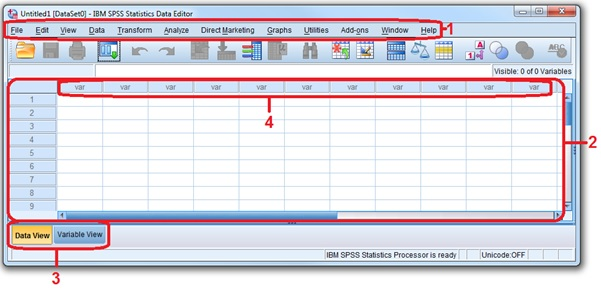
\includegraphics{C:/OneDrive - University of Leeds/Teaching/MSc IH/YCHI5045M/Teaching materials/Computer sessions/YCHI5045M practical sessions website/Images/SPSS main window.jpg}
\caption{SPSS main window view}
\end{figure}

\begin{itemize}
\tightlist
\item
  SPSS has two main windows: the data editor, as we've just seen in the image above, and the ``output window'', which displays the SPSS syntax or code that the buttons you click create to tell SPSS what to do (which you can ignore and you'll probably find annoying that it's displayed every time you do something) along with the results of those commands (usually printing tables of results from analyses and producing graphs, which are useful). This only appears once you tell SPSS to do something though. \textbf{For simplicity we will just refer to the data editor window as the main window from now on.}
\end{itemize}

\hypertarget{loading-data-in-spss}{%
\subsection{Loading data in SPSS}\label{loading-data-in-spss}}

\begin{itemize}
\item
  Next let's load some data so we can explore the main window (and the output window will appear for the first time). Go back to the main window in SPSS and in the main menu click File \textgreater{} Open \textgreater{} Data. Then in the Open Data tool window that opens navigate to the folder where you saved the ``YCHI5045M computer practical files.zip'' folders and go into the ``Datasets'' folder in the same way you would locate a folder in Windows Explorer. Find the file called ``Example basic data.sav'' and either double click on it or click on it once and then click the OK button.
\item
  This is an SPSS format dataset (.sav) and therefore contains more data and formatting of the data than other formats such an Excel (.xlsx) or .csv etc. This allows it to store things like variable labels and value codes (see below).
\item
  You will eventually see the output window appear and display some code that is telling SPSS to load the dataset, and then SPSS should take you back to the main window where you will see the raw values of the data in the Data View tab. See number 3 in the image above. The variable names are in the top row and the raw data values are in the cells. You will see there are three variables.
\end{itemize}

\hypertarget{the-main-features-of-the-main-window}{%
\subsection{The main features of the main window}\label{the-main-features-of-the-main-window}}

Refer to the ``SPSS main window view'' image above and the numbered features:

\begin{enumerate}
\def\labelenumi{\arabic{enumi}.}
\item
  The main menu. This is where you select commands to do most things you need to do.
\item
  The raw data view. Similar to Excel, here you will see the raw data displayed (although you can choose whether to display categorical variables' labels or raw values if numerically coded - see below).
\item
  These tabs allow you to either view the Data View, where the raw data is displayed in the main area (2), or the Variable View, where information about each variable is displayed and where you can edit variables' characteristics.
\item
  Variable names will be displayed here once any data are loaded.
\end{enumerate}

\hypertarget{variable-nameslabels}{%
\subsection{Variable names/labels}\label{variable-nameslabels}}

Before going further we will just set an option (or check that it's already set) in SPSS so that it displays variables' \emph{names} rather than variables' \emph{labels} in the various tools we will be using. We will see what the difference between these two things are later. This is because in the instructions below we refer to variables' names rather than their labels. However, you can certainly choose to display either for your own analyses.

\begin{itemize}
\tightlist
\item
  From the main menu bar go: Edit \textgreater{} Options and then under the General look under the Variable Lists section and select the Display names option as shown below:
\end{itemize}

\begin{figure}
\centering
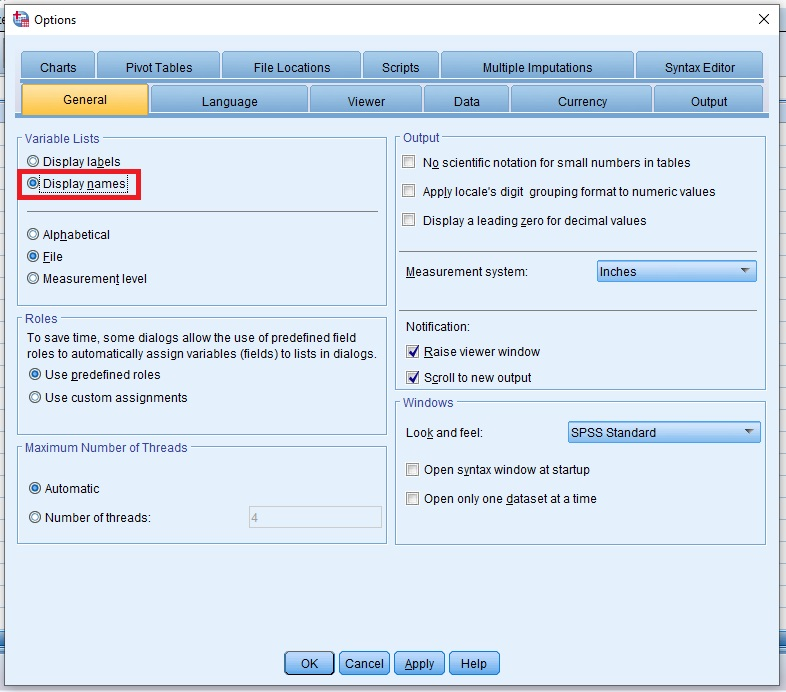
\includegraphics{C:/OneDrive - University of Leeds/Teaching/MSc IH/YCHI5045M/Teaching materials/Computer sessions/YCHI5045M practical sessions website/Images/SPSS main options.jpg}
\caption{SPSS main options variable identification options}
\end{figure}

\hypertarget{the-variable-view-and-variable-properties}{%
\subsection{\texorpdfstring{The \emph{Variable View} and variable properties}{The Variable View and variable properties}}\label{the-variable-view-and-variable-properties}}

Now that we've loaded some example data into SPSS let's look at the variable properties we can edit in the Variable View tab in the main window.

\begin{itemize}
\item
  \textbf{Name} = the variable's name. Like a file name, this should be short and descriptive and clear.
\item
  \textbf{Type} = the ``type'' of format in which the variable is stored, e.g.~numbers, string (letters and possibly numbers and/or characters) etc. Note this is just how the variable is stored, and not the type of variable in terms of categorical, numerical etc (see ``Measure'' below). You can often just ignore this and you should not alter this unless you know what you are doing!
\item
  \textbf{Width} = for string variables, width refers to how many characters a value can hold. Again you can just ignore this and should not alter this unless you know what you are doing!
\item
  \textbf{Decimals} = how many decimal places will be displayed (note: changing this does not alter how many decimal places a value actually has stored though).
\item
  \textbf{Label} = the descriptive label of the variable, used to briefly describe what the variable measures in more detail than the variable name.
\item
  \textbf{Values} = used to create or edit value labels, i.e.~labels attached to different numerical values. We'll come back to this shortly.
\item
  \textbf{Missing} = used to set or change which specific values (if any) represent different types of missing data. We will not be using this.
\item
  \textbf{Columns} = how wide the displayed columns are currently.
\item
  \textbf{Align} = whether values are left or right aligned.
\item
  \textbf{Measure} = what type of data are stored in each variable. In the terminology we've been using: nominal = a binary variable or a categorical variable with 3 or more category levels, ordinal = an ordinal categorical variable, and scale = a discrete or continuous numerical variable.
\item
  \textbf{Role} = I'm not actually sure what this does so presumably it's not anything that important and you can ignore it. Google if interested!
\end{itemize}

\hypertarget{preparing-a-dataset-for-analysis}{%
\chapter{Preparing a dataset for analysis}\label{preparing-a-dataset-for-analysis}}

The first step before doing any analysis is to understand and prepare the dataset. If you are lucky this will have been done already, but either way you should still go through this process to ensure the data really are ready for analysis. You may see this stage referred to as data preparation, data cleaning or data cleansing. These can mean different things in different contexts, but in the context of preparing a dataset for analysis we want to ensure the following:

\begin{itemize}
\item
  All variables are correctly named, labelled and set to the correct data type.
\item
  All categorical variables are correctly coded and free from obvious errors.
\item
  All numerical variables are in the correct format and free from obvious errors.
\end{itemize}

In addition there are often other key features of a dataset that must be checked prior to analysis, but these will be dataset specific and we don't have time to go into the detail here. However, one common example would be checking that any unique IDs have no duplicated values, and another would be cross checking any variables that are related to confirm they are both consistent, e.g.~compare ages with dates of birth (they should agree) etc. To save time we will just do these steps for some of the variables in the \emph{SBP Excel data} dataset to see how they are done, but then use a fully cleaned and prepared dataset for the analyses.

First we'll load a typical basic Excel dataset that lacks the extra formatting features of an SPSS format dataset, and that also contains typical errors present in raw datasets such as wrongly coded categorical variable observations and clear errors in some numerical variables, so we can see how to deal with these common issues when preparing datasets.

\hypertarget{exercise-loading-excel-data}{%
\section{Exercise: loading Excel data}\label{exercise-loading-excel-data}}

SPSS can load all the main types of data you are likely to need to load, including CSV files, Excel spreadsheets, and data files from various other statistical programs like Stata and SAS. During these practical sessions we will use datasets saved in SPSS's own format (.sav), which preserves all the useful information on things like variable names and labels, categorical variable coding labels etc that we will see explained below. However, if you use SPSS in the future it is likely you will have to load data in an Excel format at some point. Therefore, the first thing we'll learn to do is to load an Excel spreadsheet.

\href{https://youtu.be/IrLCr-Gp0sw}{Video instructions: load Excel data into SPSS}

\textbf{Written instructions: load Excel data into SPSS}

Go back to the main window in SPSS and in the main menu click File \textgreater{} Open \textgreater{} Data. Then in the Open Data tool window that opens navigate to the folder where you unzipped the YCHI5045M computer practical files and go into the ``Datasets'' folder in the same way you would locate a folder in Windows Explorer. Then to allow you to see Excel files look for the Files of type drop-down menu beneath the area in the Open Data tool where the folders and files are displayed, and select the All Files option here. Then click on the ``SBP data.xlsx'' dataset and then click Open (or double click on the file). A tool window will pop-up called Opening Excel Data Source. Ensure the Read variable names from the first row of data box is ticked and the Worksheet drop down menu is on ``SBP data {[}A1:I557{]}'' and then click OK. You will now see the raw data displayed in the Data View with the variable names in the top row and the data values in the cells. You will see there are nine variables.

\hypertarget{exercise-set-variable-properties-code-categorical-variables-and-check-categorical-variables-for-obvious-errors}{%
\section{Exercise: set variable properties, code categorical variables, and check categorical variables for obvious errors}\label{exercise-set-variable-properties-code-categorical-variables-and-check-categorical-variables-for-obvious-errors}}

Now using our ``raw'' Excel dataset (that just contains the variable names and their values) let's see how to set key variable properties, check that all categorical variables are correctly coded and free from obvious errors, and check that all numerical variables are free from obvious errors. For this we will need to understand the key details of our variables. If you are working with data that is not your own then assuming you are using a high quality, well documented dataset, this information will often be presented in the form of a ``codebook''. We will present the codebook for this dataset in the form of a table below:

\begin{table}

\caption{\label{tab:unnamed-chunk-3}*SBP data* dataset variable details}
\centering
\begin{tabular}[t]{l|l|l}
\hline
Variable name & Variable type & Variable description  (units/coding of levels)\\
\hline
id & Numerical:discrete & Observation ID\\
\hline
sbp & Numerical: continuous & Systolic blood pressure (mmHg)\\
\hline
htn & Categorical: nominal (binary) & Hypertension (SBP >= 140 mmHg, 0 = no/1 = yes)\\
\hline
age & Numerical: discrete & Age (years)\\
\hline
sex & Categorical: nominal (binary) & Sex (1 = male/2 = female)\\
\hline
ses & Categorical: nominal & Socio-economic status (1 = low/2 = medium/3 = high)\\
\hline
salt & Numerical: discrete & Salt consumption (g/day)\\
\hline
bmi & Numerical: continuous & BMI (kg/m2)\\
\hline
ace & Categorical: nominal (binary) & ACE inhibitor usage for at least 3 months (1 = yes/2 = no)\\
\hline
\end{tabular}
\end{table}

\href{https://youtu.be/ldFKC_qBFdA}{Video instructions: set variable properties, code categorical variables, and check categorical variables for obvious errors}

\textbf{Written instructions: set variable properties, code categorical variables, and check categorical variables for obvious errors}

First we'll make sure our variables are correctly named, labelled and set to the correct data type, and that all categorical variables are correctly coded. Note: for some of these exercises we will just edit a few of the variables for practice, but leave the rest alone. This is okay because when we move on we will be using a fully updated version of the dataset so we don't need to update more than enough to understand the processes. To make these updates we need to know what variables are in our dataset and what data they contain, its units/coding etc. This information would either be available to you if you were the one who collected the data, or it would be made available in a ``codebook''. Refer to the codebook table above for the key details of all variables in this \emph{SBP Excel data} dataset when updating the variables' details.

\hypertarget{variable-names}{%
\subsection{Variable names}\label{variable-names}}

\begin{itemize}
\tightlist
\item
  On the Variable View tab look at the Name column. Here you see the variables' names. Variable names are short terms used to refer to the variables, a bit like file names. Variable names should be short, clear, understandable and unambiguous. We'll leave these as they are, but just so you can see how to edit them click on the variable name ``id'', delete it and re-enter it.
\end{itemize}

\hypertarget{variable-labels}{%
\subsection{Variable labels}\label{variable-labels}}

\begin{itemize}
\item
  Next in the Variable View look along to the Label column where the variable labels can be stored (there are none in this dataset yet as Excel cannot store such information). Variable labels allow you to briefly describe the variable in more detail than the variable name. Good practice is to include the units for numerical variables or the coding scheme for categorical variables. Let's add some for practice:
\item
  For the variable sbp click on the variable label cell and enter ``Systolic blood pressure (mmHg)'', i.e.~the brief description of the variable with the units included take from the codebook table.
\item
  Now click on the variable label for ses and enter the description provided in the codebook table (you can just copy and paste it from the table).
\item
  Feel free to update the variable labels for some other variables if you wish, but once you've know how to do it you can move on.
\end{itemize}

\hypertarget{variable-types}{%
\subsection{Variable types}\label{variable-types}}

\begin{itemize}
\item
  It is very important that variable types are correctly set in SPSS (and all stats packages), because it affects the way analyses and other things like graphs may work, with incorrectly defined variable types resulting in errors. To set the variable type go to the Variable View and click on the relevant cell under Measure (it will either say ``Scale'' or ``Nominal'') and select the correct type from the drop-down menu. SPSS will set the Measure based on the nature of the variable: for any variables with any non-numeric (i.e.~letters or special characters) values the variable Type will be String and the variable Measure will be Nominal, and for any variables with only numeric (discrete or continuous) values the variable Type will be Numeric and the variable Measure will be Scale. However, these automatic choices may not be correct for the dataset!
\item
  For our dataset let's start with sbp. What do you notice about its Type and Measure? The Type is String and the Measure is Nominal. What about if you click on the Measure cell? Only nominal and ordinal options are available! This means that at least one value in the variable is non-numeric, i.e.~a letter or special character. Unfortunately there are no easy ways to check which values are non-numeric (there are ways using more complicated functions, but we don't have time for that here), but if you create a frequency table (see later for how to do this) and scroll through all the values you may be able to spot the problem values. However, to save time here the issue is observation number 93, which has a value of 1o3, i.e.~with a letter ``o'' instead of a zero.
\item
  To update the erroneous value go to the Data View and either scroll down to the value (observation 93) and update it, or click on the sbp column variable name/heading to select the whole variable, then press \textbf{ctrl} and \textbf{f} to open the Find and Replace - Data View tool (below the Find tab it should say ``Column: sbp''), then click on the Replace tab and then in the Find text box enter ``1o3'' (without the quotes) and then in the Replace text box enter ``103'' (without the quotes) and press the Replace button at the bottom to correct the value.
\item
  Once the error has been updated go back to the Variable View window and update the variable Type for sbp to Numeric, because only Numeric type variables can be Scale variables (sorry for the confusing terminology, I don't like SPSS's choices!). Click on the relevant cell for sbp under Type and click the little box with three dots that appears to the right. Then select Numeric and then OK. As there are no more values with strings or non-numeric characters in you should now be able to update the variable's Measure to Scale!
\item
  You can go through all other variables and ensure the variable \textbf{Type} and \textbf{Measure} characteristics are set correctly if you wish, but once you're happy how this is done feel free to move on.
\end{itemize}

\hypertarget{value-labels-coding-categorical-variables}{%
\subsection{Value labels: coding categorical variables}\label{value-labels-coding-categorical-variables}}

\begin{itemize}
\tightlist
\item
  Categorical variables must use some type of coding or coding scheme to be understandable. This just refers to how categorical variables' levels are stored (e.g.~our sex variable has two levels: male and female). There are two approaches:
\end{itemize}

\begin{enumerate}
\def\labelenumi{\arabic{enumi}.}
\item
  String/character coding: each categorical level is referred to via a string (i.e.~a set of letters, numbers or special characters). E.g. sex might take either the value ``male'' or ``female''.
\item
  Value coding: each categorical level is referred to via a number, with the number linked to a ``value label'' that then describes what that level represents. E.g. sex might take either the value 1 or 2, where 1 is linked to the value label ``male'' and 2 is linked to the value label ``female''.
\end{enumerate}

\begin{itemize}
\item
  You can use either approach in SPSS and you shouldn't have any problems. However, as value coding is often used and requires more understanding of SPSS to add/edit we will follow this approach so you can get the practice.
\item
  So let's set-up value labels for our categorical variables sex and ses. To do this we must ensure that they are correctly coded with numbers and that suitable value labels are attached those numbers. In ``real life'' we would repeat this process for all other categorical variables. Before making any changes though we must first check each categorical variable to find out what levels exist and if there are any errors -- you might be surprised. The easiest way to do this is to generate a frequency table: a table listing the number of cases the percentage of cases with each level.
\item
  From the main menu go: Analyze \textgreater{} Descriptive Statistics \textgreater{} Frequencies. Note that SPSS tries to work out the type of variable based on the values present, e.g.~if there are any non-numerical characters it will assume a categorical variable. In SPSS categorical variables are represented by three coloured circles, and numerical variables by a small ruler symbol. However, these assumptions will not necessarily be correct. Let's look at sex and ses. Either double click on the sex and ses variables in turn or click once on each while holding the \textbf{shift} button and then click the right pointing arrow to add them. Then ensure the Display frequency tables button is ticked and click OK. The results will appear in a new output window, which is the other main window in SPSS where all results will be displayed along with any error messages.
\item
  Now look at the frequency table to see what levels are present for sex and ses and how they are coded. Note that sex has been entered as a string variable (with levels recorded as words) and ses has been entered as a numeric variable (with levels recorded as numbers). Now you can see why frequency tables are so useful for data cleaning. For sex you can see that there are five levels, and it's clear that three are errors (both the fact there are clear spelling mistakes/odd values and the fact they only occur once indicate they are mistakes). Specifically the levels ``\emph{1}'', ``\emph{FM}'' and ``\emph{mal}'' need correcting.
\item
  We therefore need to first clean/correct the error values, and then convert all values to numerical values and then add the labels. Look at the codebook above and the ``Description (units/level coding)'' column for the correct coding to apply to each level. To correct the mistakes go back to the Data View and click the top of the sex column (click on the word sex) to highlight the whole column. Then hold \textbf{ctrl} and \textbf{f} to open the Find and Replace - Data View tool. Then in the Find text box enter ``1'' (without quotes) and in the Replace with text box enter ``male'' (without quotes) and then click Replace All. Repeat this find and replace process for all other levels that are errors with the obvious correct word. Then use the find and replace process to change all ``male'' values to the number 1, and all ``female'' values to the number 2. We can now add value labels to these numerical codes. Be sure to add labels to the correct numerical values or they won't display.
\item
  Now go back to the main window Variable View and click on the Values cell for sex where it currently says ``None''. You'll see a small box appear to the right of the cell with three dots in it -- click on this to open the Value Labels tool. Then click the Value text entry box and type 1. Then click the Label text entry box and type ``male''. Then click Add. Then repeat for Value = 2 and Label = ``Female'' (make sure you remember to click Add). Then once both value labels are added click OK.
\item
  Next let's correct (if necessary) and code ses. Go back and look at the frequency table for ses. We can see there are four levels with one obviously incorrectly coded level of ``11'' only observed once. Clearly this should be coded as ``1''. Use the find and replace process detailed above to replace level ``11'' with ``1'', and then attach the correct value labels to the levels 1, 2 and 3 based on the information provided in the codebook table (1 = low, 2 = medium and 3 = high).
\item
  Note: variable labels and value labels are not stored in Excel files, so to retain them you must first save your dataset in SPSS ``.sav'' format. This can be done by going from the main menu to: File \textgreater{} Save As, and then selecting a folder and file name. The .sav format should be the default selected, but ensure that you save your updated dataset in this format.
\end{itemize}

\hypertarget{exercise-check-numerical-variables-for-obvious-errors}{%
\section{Exercise: check numerical variables for obvious errors}\label{exercise-check-numerical-variables-for-obvious-errors}}

\href{https://youtu.be/Q51ex9lcqJs}{Video instructions: check numerical variables for obvious errors}

\textbf{Written instructions: check numerical variables for obvious errors}

\begin{itemize}
\item
  All we can really hope to find are clearly erroneous values, such as values that are outside the plausible range of values for the variable based on what it is measuring or what we restricted it to via study design, but more modest errors won't be detectable.
\item
  If you have a numerical variable with relatively few distinct/unique values, such as age, then probably the easiest check is another frequency table. Produce a frequency table for age and what do you notice about the extreme values (i.e.~the lower and upper ends)? One person has an age of 4. This is clearly an error, as the study only recruited participants aged 18+. What to do? There are three choices: 1) leave it as it is, 2) update it or 3) delete it. Option 1 is not a good idea because we know it must be an error. Option 2 would be ideal, but you can't always do this. In this case an age of 4 could actually be an age of 24, 34, 40, 41 etc, so we would have to be able to go back and contact the participant to check their age if we wanted to update this. Where this is not possible you could conduct a sensitivity analysis by running your analysis with this age value as 40 and then again with the value updated to 49. That way you see what happens when you assume it was actually either end of the possible value range of the likely true value. Or you may take option is 3 and delete the value (but this should be reported in your methods). However, here we'll assume we were able to check and the correct age should have been 40. To update this go to the Data View, right click on the age variable name and select Sort Ascending. The data should now be ordered with the participant with age 4 at the top (or you could use the find and replace process detailed above). Update their age to 40.
\item
  When numeric variables have lots of different unique values, such as when they include decimals, using a frequency table becomes less easy. A better option is to produce a dotplot (also called a dotchart or Cleveland dotplot/dotchart), which is like a histogram but each value is displayed as a dot, with dots from observations of values in a similar range (i.e.~in the same ``bin'') being stacked like a histogram. As BMI has very few (maybe no) repeated values a frequency table will be huge. Let's produce a dotplot instead. From the main menu go: Graphs \textgreater{} Legacy Dialogues \textgreater{} Scatter/Dot. Then click Simple Dot \textgreater{} Define. Then in the Simple Dot graph tool add the variable bmi into the X-Axis Variable box. Then click OK. Looking at the graph you'll see a huge stack of values of similar values, and then far out to the right on the x-axis you should clearly see an anomalous value (a circle) that must be an error because it's so high. Double click on the graph which will open it in a new window where you can edit the graph. Now click on the error value, which should highlight all circles in yellow, and then click on it again and only the error circle should be highlighted. Then right click on the circle and choose Go to Case. This will take you to the relevant observation in the Data View where you can update it. Again we have three choices, and let's assume we could go back and get the correct value either from the participant or an earlier dataset (e.g.~if weight and height were measured separately), and it was actually 28.175.
\item
  Now re-run the dotplot for BMI and what do you see? Again there is a value to the right of the distribution that is a far way to the right (higher) than any other BMI value. This may be considered an ``outlier''. Outliers are extreme values that are far greater/smaller than any other values in a numerical variable. There are no clear thresholds beyond which a value is considered an outlier, but as you can see probably the easiest way to spot possible outliers is via a dotplot. Once you've identified any possible outliers such as this very high BMI value you should check to see if they are obvious errors and correct them if possible. However, if they appear to be genuine values the recommended approach is to conduct any analyses that involve the relevant variable(s) with and without the outliers present, i.e.~repeat your analysis but delete the observations (e.g.~individuals) who have the outliers and see what changes. Then simply clearly report the results of both of these analyses and any implications for the interpretation of your results. This is known as a sensitivity analysis. Broadly speaking, if removing outliers makes an important difference for your results then your results are probably not very robust to start with. Where you have plenty of good quality data removing the odd outlier from an analysis will rarely make much difference unless it's a relatively hugely larger/smaller value. As you'll have seen from the dotplot there are no outliers in this dataset.
\end{itemize}

\hypertarget{a-final-note-on-data-cleaning}{%
\section{A final note on data cleaning}\label{a-final-note-on-data-cleaning}}

We will end our data cleaning there having seen how to clean and prepare all variables as best as we can in isolation. However, with a real dataset these steps would just be the basics, and we would want to look further to check for errors and anomalous values by also looking at relationships between variables. For example, if we looked at a scatter plot of sbp \textasciitilde{} age we may see a suspiciously high value for sbp for a very young participant, i.e.~one that would be very unlikely in such a young individual. We could then check this with any prior data or the participant if we were able to.

\textbf{Note: it's considered a good rule that you should only delete an observation from a given variable if you can confirm beyond reasonable doubt that it is an error, and that any data deletions must be reported in any results section of a paper/report etc. If you are concerned that one or more observations for one or more variables are errors but you cannot confirm this then a good approach is to run your analyses with and without those data points, and then in your results explain if this made any difference to your conclusions and discuss the implications accordingly.}

\hypertarget{describing-a-dataset}{%
\chapter{Describing a dataset}\label{describing-a-dataset}}

\hypertarget{background}{%
\section{Background}\label{background}}

Once you have a nice, clean, correctly set-up dataset, the first step in any data analysis is to describe your dataset with descriptive statistics and/or graphs. This is often done in two somewhat distinct stages. In the first stage researchers usually just describe all the variables in their data on their own, producing what are known as univariate descriptive statistics (where univariate means ``single variable''). Then in the second stage they may often look at relationships between variables, with bivariate analyses looking at relationships between two variables at a time, and multivariate analyses (less commonly done in analyses involving descriptive statistics) looking at relationships between three or more variables at a time. Note: there is some cross-over with the data cleaning stage, e.g.~we already produced a scatter plot to check for anomalous values in the numerical variables. The main reasons for doing this descriptive analysis is:

\begin{itemize}
\item
  First, this allows you understand your variables (e.g.~their data type and distributions) and also often the relationships between them, which helps you plan your inferential analyses.
\item
  Second, this allows you to describe what the sample ``looks'' like in terms of its key characteristics. E.g. in our dataset we will describe the key bio-medical and socio-demographic characteristics of the sample, while in a study on e.g.~health facility outcomes you might have data that allows you to describe a range of key facility characteristics, such as the number of beds, the number of staff, frequency of drug stock outs etc. Describing the sample's characteristics then allows readers to understand who was in the study and who the results can be generalised to. E.g. in our study the descriptive statistics for age show that all participants were aged 18 to 60, and that most of the participants were between their early 20s to late 50s. Therefore, clearly the results can only be formally and robustly generalised to individuals from the same setting who are also between 18 to 60, and probably most robustly to those individuals between their 20s and 40s, i.e.~not to individuals from the same setting who are adolescents (very young) or geriatrics (very old). And when you start trying to generalise results beyond your setting and context you need to be very careful and think very carefully about how valid those generalisations are.
\item
  Note: when descriptively exploring variables to understand your data and plan your analyses it is recommended to make extensive use of not just numerical descriptive statistics but also graphs, because we can easily understand and process information visually. However, graphs are not typically used in papers for describing samples, mainly due to space constraints. The most commonly used graph to describe a single numerical variable is a histogram, and the most commonly used type of graph to describe a single categorical variable is a bar chart.
\end{itemize}

If you are still unclear on the difference between descriptive statistics and inferential statistics, or want a brief refresher, you can read the below information.

\hypertarget{descriptive-vs-inferential-statistics}{%
\subsection{Descriptive vs inferential statistics}\label{descriptive-vs-inferential-statistics}}

It's important to be very clear on the distinction between descriptive and inferential statistics. Descriptive statistics simply describe the characteristics of variables or the relationships between variables in your sample, i.e.~the dataset you have collected, and they do so \emph{without any uncertainty}. They consist of ``point estimates'', or statistics that take single values, such as means and percentages. However, they do not allow you to make robust generalisations about the characteristics of variables or the relationships between variables in the target population (or more widely if plausible) from which the sample was taken. To do that requires inferential statistics such as (most commonly) confidence intervals and p-values. Note though that inferential statistics are usually presented and interpreted along with relevant descriptive statistics to allow inferences to be made. For example, confidence intervals are usually presented \emph{around a relevant point estimate or descriptive statistic}, where the point estimate is taken as the single best estimate of the likely value of the population parameter and the confidence intervals provide a range of values that are consistent with the likely value of the population parameter.

This terminology can be a source of confusion particularly for survey-type studies, where we often say we are aiming to \emph{describe} the characteristics of a given target population, but what we mean is we are going to use inferential statistics (typically confidence intervals around our point estimates) to say something about the likely characteristics of our target population (i.e.~to describe their likely characteristics). However, we are not implying that we are going to use descriptive statistics alone to do this, as descriptive statistics (i.e.~point estimates such as means and percentages) on their own don't allow us to say anything robust about the likely characteristics of our target population.

To illustrate the difference: if we have a list of all post-graduate students of the University of Leeds and we take a simple random sample of 100 of those students and measure their blood pressures (mmHg) we can calculate the mean blood pressure for the sample exactly (i.e.~the mean blood pressure of the sample would be a descriptive statistic describing the typical value of blood pressures in the sample). Similarly, if we were able to measure all of the students' blood pressures we could then also calculate the exact mean blood pressure for the target population, i.e.~all UoL post-graduate students, which would also be a descriptive statistic describing the target population. But in practice such a census is not possible. Therefore, if we want to say something about the likely mean blood pressure in the target population, i.e.~all post-graduate students at the UoL, based on our sample alone we need to use inferential statistics. For inferring characteristics about single variables we typically calculate the relevant sample statistic from the sample, which is just identical the descriptive statistic, and is the best single or ``point estimate'' of the likely parameter of interest (e.g.~the mean) in the target population (assuming a random sample, or more technically a probability sample). For our example this would be the mean blood pressure (mmHg). Then to allow us to make inferences/generalisations to our target population, that we took our sample from, we could estimate confidence intervals (usually 95\% CIs) around that sample statistic. In other situations, for inferring relationships between variables we might estimate the difference between two variables or the correlation or a regression coefficient, which again are all sample statistics and on their own can be used as descriptive statistics, but for inference we would then also compute the relevant confidence intervals, and maybe also compute p-values where there are useful null hypotheses that we can test about those statistics.

\hypertarget{exercise-create-descriptive-statistics}{%
\section{Exercise: create descriptive statistics}\label{exercise-create-descriptive-statistics}}

\begin{itemize}
\tightlist
\item
  Load the ``SBP data final.sav'' SPSS dataset. This has all the errors removed from the ``SBP Excel data.xlsx'' dataset we looked at last session, and all the variable properties like variable labels and value labels etc have been updated.
\end{itemize}

\hypertarget{overview-9}{%
\subsection{Overview}\label{overview-9}}

In the YCHI5045M computer sessions materials ``Exercises'' folder also open the ``Exercises.docx'' Word document and scroll down to \textbf{Descriptive statistics table}. The aim of this exercise is to complete the empty table by calculating the values of the relevant descriptive statistics for the variables in the table (i.e.~the key variables in the dataset). Note: the footnotes to the table are typical of such tables in papers and allow us to just present a single column of descriptive statistics. However, you could of course present the values in other ways. Once you've completed your table you can compare it to the completed one at the end of this section to see how you did.

For each type of variable (numerical or categorical) calculate and present the following descriptive statistics, which are typically presented in ``Table 1'' of a paper to describe a sample's characteristics:

\begin{itemize}
\item
  Numerical variables: if the variable is approximately normally distributed calculate the mean and the standard deviation (SD), and if the variable is skewed calculate the median the interquartile range (IQR). In tables the convention is to present the mean and then in brackets after the mean the standard deviation, or the median and then in brackets after the median the standard deviation. E.g. for a mean of 10 mmHg and a SD of 2.5 you would write: 10 (2.5). The units can either be given after the mean or just included in the variable description like in the table.
\item
  Categorical variables: simply calculate the frequency (count) and the percentage (or proportion, but percentages are typically used) for each category level. E.g. for the variable sex calculate the frequency and the corresponding percentage of individuals who are male and female.
\item
  Present values just to 1 decimal place. We have completed the first two variables for illustration.
\end{itemize}

See below for instructions about how to do this in SPSS.

\href{https://youtu.be/uw0ukUUKg5o}{Video instructions: calculate common descriptive statistics}

\textbf{Written instructions: calculate common descriptive statistics}

\hypertarget{categorical-variables}{%
\subsection{Categorical variables}\label{categorical-variables}}

\begin{itemize}
\tightlist
\item
  To calculate descriptive statistics for the categorical variables we just need to produce frequency tables for each variable and extract (i.e.~copy) the counts for each category level and the corresponding percentages. Simple! From the main menu go to: Analyze \textgreater{} Descriptive Statistics \textgreater{} Frequencies. Then in the Frequencies tool window add all categorical variables to the Variable(s): box. You can either drag each variable across one-by-one by clicking and holding down the left mouse button, or you can click on each one and then click the button in between the two boxes to move it over (or to move it back), or you can select multiple variables and move them at the same time in the same way by first holding down \textbf{ctrl} and then clicking on as many variables as you want to before moving them. Note: this is the typical behaviour of these types of variable boxes in SPSS and you will spend quite a lot of time moving variables so it's good to try the different methods. Once you have moved all the categorical variables in the table over to the Variable(s): box just ensure the Display frequency tables box at the bottom of the tool is ticked and then click OK. After a moment in the output window you should see the tables appear (one for each variable). You can now copy the relevant values from the \textbf{Frequency} and \textbf{Percent} columns into the table.
\end{itemize}

\hypertarget{numerical-variables}{%
\subsection{Numerical variables}\label{numerical-variables}}

\begin{itemize}
\item
  Now for numerical variables. First we need to check the variables' distributions to see whether they are approximately normal or skewed. There are statistical tests that can be used to formally test whether a variable's distribution differs ``significantly'' from a normal distribution, but as they are based on p-value thresholds the result depends strongly on the sample size, and with a big enough sample size you are essentially guaranteed that a variable will fail the test and be classed ``non-normal''. However, many statistical tests that rely on normality are quite robust to modest (or sometimes worse) departures from normality, i.e.~they still work well with slightly skewed variables and have much more power than equivalent non-parametric tests. Therefore, it's better to judge normality by eye using histograms even if this seems unscientific or less robust than using a statistical test.
\item
  So let's see how to create histograms for numerical variables to check their distributions. In the main menu go: Graphs \textgreater{} Legacy Dialogues \textgreater{} Histogram. Then add the sbp variable into the Variable: box and tick the Display normal curve box just below the Variable: box. This adds a curved line to the histogram which shows what the distribution of values would look like assuming the data were normally distributed. If the histogram follows this fairly well we can assume approximate normality. Now just click OK. Do this for each numerical variable in turn and examine the graphs. What do you see? sbp, age and bmi all appear to approximate a normal distribution well, but salt displays some slight right skew. Therefore, let's present the mean and SD for sbp, age and bmi, and the median and IQR for salt. Go: Analyze \textgreater{} Descriptive Statistics \textgreater{} Explore. Then in the Explore tool window add each numerical variable to the Dependent List: box. Then click the Statistics button and ensure the Descriptives box is ticked and click Continue. Then back at the main Explore tool window in the Display options at the bottom ensure the Statistics option is selected and then click OK. You'll then get several tables produced in the output window, one for each variable, with lots of descriptive statistics listed. Simply copy the relevant statistics (mean/median and SD/IQR) from them and add them to your Table 1.
\end{itemize}

\hypertarget{example-completed-table}{%
\subsection{Example completed table}\label{example-completed-table}}

\begin{figure}
\centering
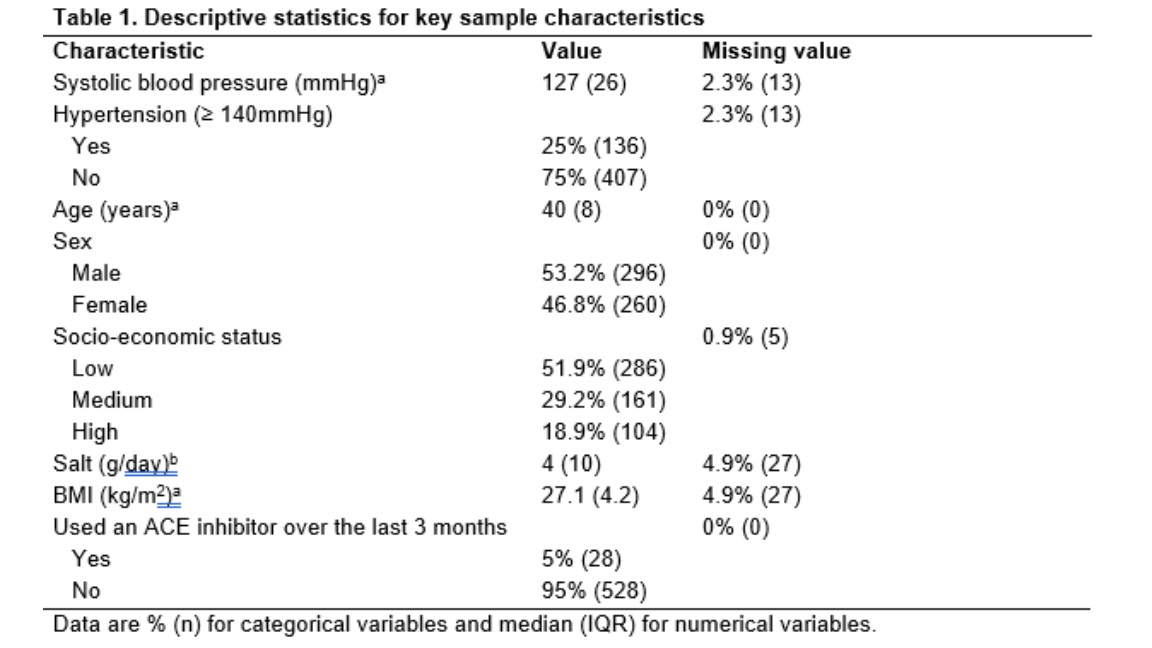
\includegraphics{C:/OneDrive - University of Leeds/Teaching/MSc IH/YCHI5045M/Teaching materials/Computer sessions/YCHI5045M practical sessions website/Images/Table 1.jpg}
\caption{Completed Table 1 for SBP dataset}
\end{figure}

If you have any glaring errors or strange differences try and work out why, and if you can't then ask for help!

\hypertarget{the-independent-t-test}{%
\chapter{The independent t-test}\label{the-independent-t-test}}

\hypertarget{overview-10}{%
\section{Overview}\label{overview-10}}

The independent t-test allows you to compare whether two independent groups differ in their mean values of some numerical outcome, or less formally whether individuals in one group have higher/lower values for some numerical outcome than individuals in another group, on average. Therefore, it is suitable when your outcome is numerical and your single independent variable is binary. For example, if you wanted to analyse whether a group of women had a different mean systolic blood pressure from a group of men. Therefore, the independent t-test is suitable for when your outcome is numerical and your independent variable is binary. Strictly speaking the outcome should be continuous and normally distributed for each group, but the independent t-test is very robust to non-normally distributed outcomes and as long as the outcome isn't strongly skewed for each group it should be okay to use this test. Note: with the independent t-test the independent variable is binary and might naturally consist of a categorical variable with just two levels (like sex), or we might construct a binary variable from a categorical variable with \textgreater2 levels (e.g.~reclassifying socio-economic status from low, medium and high levels to just low/medium and high levels by pooling individuals in the low and medium levels), or we might create a binary variable from a numerical variable based on a threshold cut-off (e.g.~BMI ≤20 vs BMI \textgreater20). We'll look at the last of these scenarios as it requires a bit more preparation, so you will know how to do this if needed in SPSS.

\hypertarget{scenario-7}{%
\section{Scenario}\label{scenario-7}}

Using the SBP final dataset we'll see how we can use the independent t-test to compare whether the mean systolic blood pressure (mmHg) differs between individuals aged ≤40 compared to those aged \textgreater40, and then you can try a similar analysis by yourself.

\hypertarget{step-1-create-a-binary-independent-variable-from-a-numerical-variable}{%
\section{Step 1: create a binary independent variable from a numerical variable}\label{step-1-create-a-binary-independent-variable-from-a-numerical-variable}}

\begin{itemize}
\tightlist
\item
  Load the ``SBP data final.sav'' SPSS dataset.
\end{itemize}

\href{https://youtu.be/DPphng9PC4Q}{Video instructions: create a binary independent variable from a numerical variable}

\textbf{Written instructions: create a binary independent variable from a numerical variable}

Next we need to create a two-level categorical variable defining our younger and older individuals. Usually you should choose the cut-point at which you define your two-levels based on theory or some sensible motivation (e.g.~the age at which prior research suggests blood pressure may often change), but here let's just compare those individuals above and below the \emph{median age}, which is 40. We therefore want to create a variable that classifies every individual as either ≤40 or \textgreater40.

\begin{itemize}
\tightlist
\item
  First, we can use the Compute Variable tool to create a new variable based on a logical test of whether the value in the original age variable is ≤40 or not. This will create a new variable that has the value 0 if the participant's age is \textgreater40 and the value 1 if their age is ≤40 (i.e.~if the logical check we asked SPSS to do on the original age variable is TRUE then the new variable's value is 1). From the main menu go: Transform \textgreater{} Compute Variable. Then in the Compute Variable tool enter ``age\_young\_old'' as the name for the new variable in the Target Variable: box. Then in the Numeric Expression: box enter:
\end{itemize}

\begin{quote}
age \textless= 40
\end{quote}

Then click OK.

\begin{itemize}
\item
  The output window will appear. Minimise this to go back to the main window and go to the Variable View. You should now see our new variable age\_young\_old has appeared. Let's give it a variable label so it's well described in SPSS: Age (0 = \textgreater40 / 1 = \textless=40). Then let's give it some value labels so each level is well described. As it was created from a logical expression it takes only two values: 0 or 1. 1 should be coded as ``≤40'', because when the participant's age was less than or equal to 40 the logical expression would be true and the new variable would take the value 1. Similarly 0 should be coded as ``\textgreater40'' as the logical expression would be false and the value set to 0. Check back to the instructions on adding value labels or ask if you need help.
\item
  Lastly, once that's done you should always do a quick check that the variable has been created correctly using a ``cross tabulation'' between our old and new age variable. In the main menu go: Analyse \textgreater{} Descriptive Statistics \textgreater{} Crosstabs. Then in the Crosstabs tool add the original age variable into the Row(s): box and the new categorical binary age variable into the Column(s): box and click OK. If you've created the new age variable correctly all ages ≤40 should be counted in the age \textless=40 column and all ages \textgreater40 in the new age variable age \textgreater40 column. Always perform such checks when creating new variables!
\end{itemize}

\hypertarget{step-2-check-the-assumptions-of-the-independent-t-test-are-not-violated}{%
\section{Step 2: check the assumptions of the independent t-test are not violated}\label{step-2-check-the-assumptions-of-the-independent-t-test-are-not-violated}}

Whenever you run a statistical analysis you must ensure that the assumptions of the analysis are not violated, otherwise the results may not be valid or even meaningful. For simple analyses like the independent t-test we can check the assumptions before we run the test, but for more sophisticated analyses such as regression models we typically check the assumptions after running the analysis because SPSS produces the information to make the necessary checks only after running the analysis.

The independent t-test makes the following assumptions:

\textbf{1. Continuous outcome}

Technically an independent t-test assumes a continuous outcome variable, but as long as assumptions 2 and 3 below are satisfied it's fine to use a discrete outcome with an independent t-test. Here our outcome is continuous. Note: ideally when analysing a discrete outcome you would use a more specific model like a Poisson or negative binomial model, but this is beyond the scope of this introductory course.

\textbf{2. Independent groups (hence the ``independent t-test'')}

This means the observations in each group cannot be related. You can only really verify this by knowledge of your study design. With the SBP data the study took a \textbf{simple random sample} of individuals and we are then dividing them into two groups based on an age threshold. Therefore, by definition the two groups are statistically independent as all observations represent separate, randomly sampled individuals.

Typically groups are only not independent in two situations. First, if you were taking repeated measurements from the same set of individuals but treating the measurements at each time period as different ``groups''. Here there would be correlations between the measurements at the different time periods within individuals. Second, if you were taking measurements from two groups of separate individuals, but the individuals in the two groups were not statistically independent. For example, if there were different families with members in both the age groups, or if there were individuals from the same work places within each group. Again, in such situations there would be correlations between members of the same family or work place (e.g.~due to genetics or shared risk factors etc).

Here our groups or observations are clearly independent as the individuals in the study were randomly sampled and the two groups contain separate individuals.

\textbf{3. The outcome is approximately normally distributed within each group}

Note: technically it is the ``residuals'' or ``model errors'' that need to be normally distributed, which are the differences between the observed values of the data and the ``model predicted values''. For a t-test these are simply the differences between the observed values of the data and the mean of the relevant group that the observation comes from, which actually means that for a t-test the residuals are identical to the observed values and so you can just view the distribution of the observed data. For more complicated regression models we'll see that we need to calculate and plot the residuals separately.

To check the distribution of the residuals within each group you can use statistical tests, but most statisticians would recommend using graphical methods. We can visually check these two distributions easily in SPSS using histograms as follows. From the main menu go: Graphs \textgreater{} Legacy Dialogues \textgreater{} Histogram. Then add the sbp variable into the Variable: box, then add the age\_young\_old variable into the Rows: box, tick the Display normal curve box and then click OK. You'll see a histogram for the sbp variable for each age group. As you can see the outcome approximates a normal distribution fairly well for the ≤40 age (this is probably as good as you would see with real data), and is slightly right skewed for the \textgreater40 age group. However, as previously mentioned the t-test is pretty robust to slightly skewed outcomes so this is nothing to worry about, and we can assume this assumption is met. Below are some examples of suitably and unsuitably distributed data for you to compare with for future reference.

\textbf{Examples of suitably and unsuitably distributed data for t-tests}

Students (and researchers) often struggle with knowing whether an analysis's assumptions have been violated or not, and for good reason because it usually involves judgement based on experience. For the t-test like most analyses requiring normality there is no agreed ``threshold'' for when the skewness of a variable is considered ``non-normal''. However, as t-tests and regression models are fairly robust to some non-normality the following examples should hopefully give you a sense of when you are okay to go ahead and when you are violating the assumptions and need to transform the data or use a different model.

\textbf{A. Probably suitably \emph{approximately} normally distributed data within each group for a t-test, with n = 50 per group:}

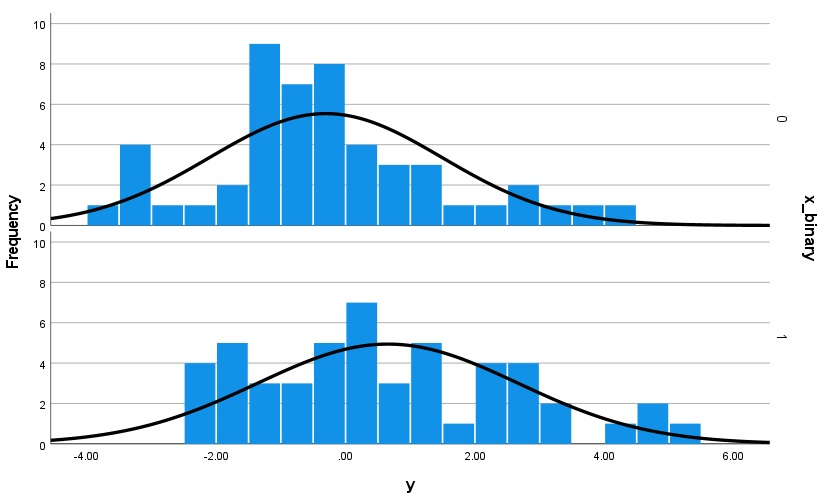
\includegraphics{C:/OneDrive - University of Leeds/Teaching/MSc IH/YCHI5045M/Teaching materials/Computer sessions/YCHI5045M practical sessions website/Images/t-test normal equal data n=100.jpg}

With only 50 data points per group the distribution is pretty ``lumpy'' but you can see an approximate normal distribution in both groups, although less so for the lower group. Also note: these data are generated from a normal distribution, so you can see that when your sample size is low even with artificially simulated data from a known normal distribution the resulting sample can often be only somewhat approximately normal! You can also see that the variance in both groups looks approximately normal, which satisfies our next assumption (see below).

\textbf{B. Highly suitably normally distributed data within each group for a t-test, with n = 500 per group:}

\begin{figure}
\centering
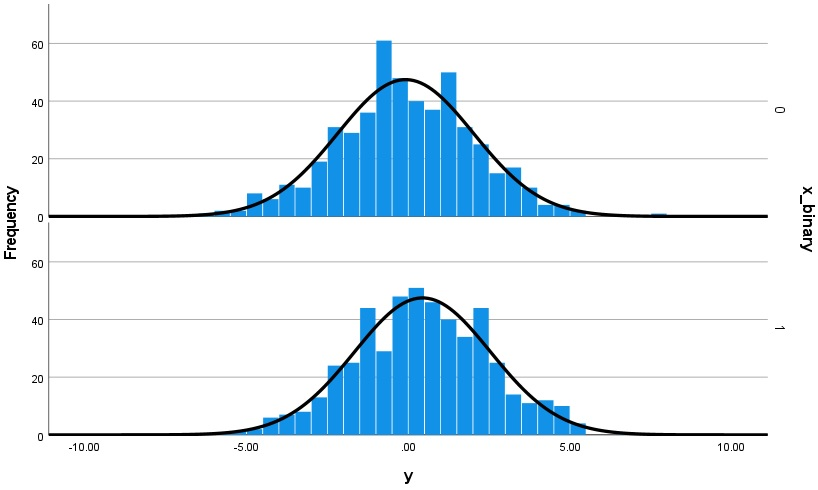
\includegraphics{C:/OneDrive - University of Leeds/Teaching/MSc IH/YCHI5045M/Teaching materials/Computer sessions/YCHI5045M practical sessions website/Images/t-test normal equal data n=1000.jpg}
\caption{Normal (and equal variance) data in each group of a t-test, n = 500 per group}
\end{figure}

Now with 500 data points per group simulated from the same distribution unsurprisingly the distribution looks much more suitably normal.

\textbf{C. Probably not suitably normally distributed data within each group for a t-test, with n = 50 per group:}

\begin{figure}
\centering
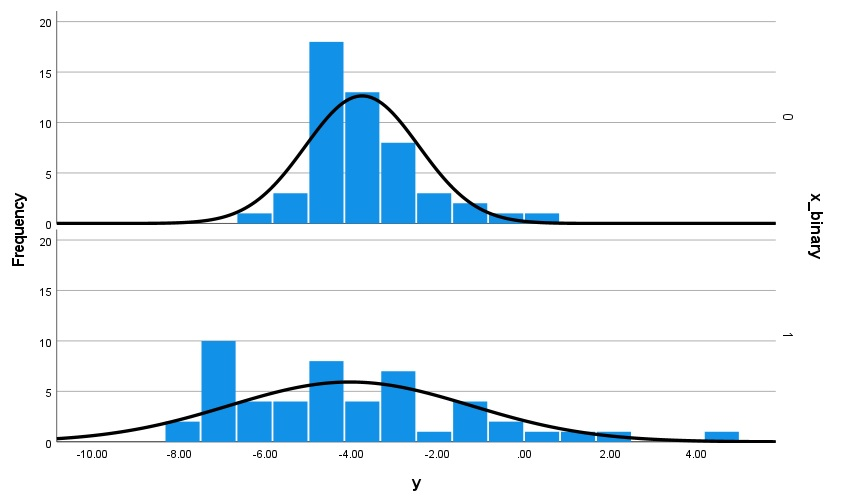
\includegraphics{C:/OneDrive - University of Leeds/Teaching/MSc IH/YCHI5045M/Teaching materials/Computer sessions/YCHI5045M practical sessions website/Images/t-test non-normal non-equal data n=100.jpg}
\caption{Non-normal (and non-equal variance) data in each group of a t-test, n = 50 per group}
\end{figure}

You may think it doesn't look much different from the first image, and you'd be right. Again, it comes down to judgement but when sample sizes are small there's a lot of subjectivity involved. These data are simulated from a right-skewed ``version'' of the normal distribution. If you are concerned one option is to run your test on the raw data and then transform the data (we'll see later how to do this) and re-run the test and see if the results change much, and just report both. This is called a sensitivity analysis.

You can also see that there is a lot more variance in the lower group's data, which would violate our next assumption (see below).

\textbf{D. Definitely not suitably normally distributed data within each group for a t-test, with n = 500 per group:}

\begin{figure}
\centering
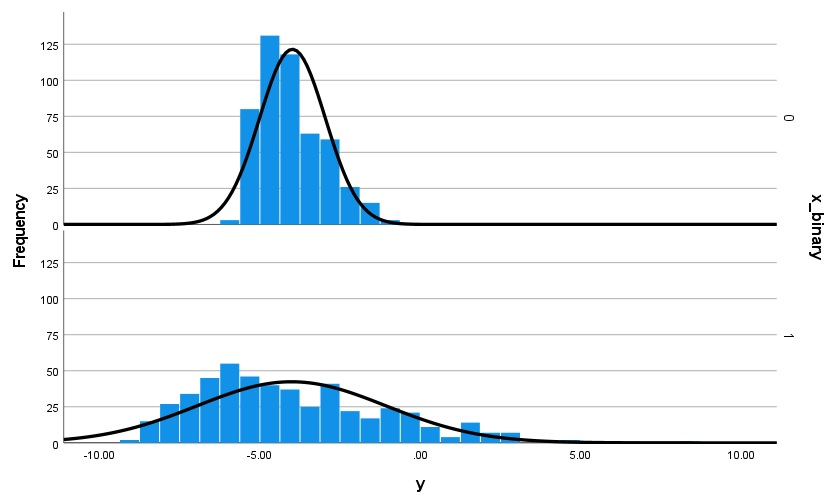
\includegraphics{C:/OneDrive - University of Leeds/Teaching/MSc IH/YCHI5045M/Teaching materials/Computer sessions/YCHI5045M practical sessions website/Images/t-test non-normal non-equal data n=1000.jpg}
\caption{Non-normal (and non-equal variance) data in each group of a t-test, n = 500 per group}
\end{figure}

Now with 500 observations per group it's clear that there is some definite right-skew in the distribution of both group's data, and that there is considerably more variance in the lower group.

\textbf{4. Equal variances in each group}

This means that the variance (dispersion or spread) of outcome values is approximately the same in each group. We can check this by looking at the p-value for a test of this assumption called ``Levene's test of equality of variances'' or by comparing the histograms from the two groups. SPSS produces the results of the Levene's test when we run the t-test, so we will evaluate the results of this test/assumption once we've produced our t-test results below. Note: if this test is significant (P\textless0.05) we can simply use the results from the version of the t-test that doesn't assume equal variances in each group. The only disadvantage is that we lose a little bit of statistical power, but typically it's not much and the results will be very similar. Hence, although we'll interpret the ``equal variances assumed'' version of the t-test below it's probably a better practice to just always use the more conservative but robust and safer set of results that do not assume equal variances is each group.

\hypertarget{step-3-run-the-independent-t-test}{%
\section{Step 3: run the independent t-test}\label{step-3-run-the-independent-t-test}}

\href{https://youtu.be/jHGKbgDWuio}{Video instruction: run the independent t-test}

\textbf{Written instruction: run the independent t-test}

\begin{itemize}
\item
  In the main menu go: Analyse \textgreater{} Compare Means \textgreater{} Independent Samples T Test. Then in the Independent-Samples T Test tool add the sbp variable into the Test Variable(s): box. Then add our new independent variable for age group (at the bottom of the list) into the Grouping Variable: box and click Define Groups\ldots{}. This is where we tell SPSS what numerical values code for each of our two groups, and what way round we want to compare the two groups. Remember we created the age variable so that it took the value ``0'' for individuals \textgreater40 and ``1'' for individuals ≤40. Let's compare individuals \textgreater40 to individuals ≤40. When it comes to comparing the groups this tells SPSS subtract the mean outcome in group 0 from group 1, i.e.~the mean systolic blood pressure for individuals \textgreater40 minus the mean systolic blood pressure for individuals ≤40. To do this ensure the Use specified values option is selected and add the value ``0'' to Group 1: and the value ``1'' to Group 2:.
\item
  Note: you can of course swap the coding values around and compare individuals ≤40 to individuals \textgreater40 and your results will be reversed but otherwise identical. Neither choice is necessarily ``correct'' it just depends on which way round you want the groups compared. If, in your version of SPSS, there is a box called Estimate effect sizes below the Grouping variable: options make sure this is not ticked. Finally click Continue and then OK. You'll now see the output window appear with our results!
\end{itemize}

\hypertarget{step-4-understand-the-results-tables-and-extract-the-key-results}{%
\section{Step 4: understand the results tables and extract the key results}\label{step-4-understand-the-results-tables-and-extract-the-key-results}}

Now we've verified the first two assumptions of the independent t-test (independent observations and approximately normally distributed residuals) let's look at the results tables where we can check the third assumption (equal variances in each group), extract the key results and interpret them.

So what do the tables mean?

\textbf{Group Statistics table explained}

The first table we see gives us descriptive statistics for the outcome variable for each level of our categorical independent variable.

\begin{itemize}
\item
  First, make sure you look at and record the values under the ``N'' column, which are the group sample sizes, and check they match what they should be. You should see there were 295 individuals in the ≤40 group and 248 individuals in the \textgreater40 age group. These sum to 543, which is less than the total number of individuals in the dataset: 556. There are three reasons why this might be: either some individuals are missing values for the outcome or the independent variable or both variables. We know from when we prepared the dataset that some individuals are indeed missing values for their systolic blood pressure. You can quickly check this by going to the Data view, right clicking on the sbp variable and selecting Descriptive Statistics. In the \textbf{Statistics} results table that appears you should see that there are indeed 13 individuals with missing values for sbp, and hence only 543 individuals with complete data on this variable, which explains the sample size of the independent t-test.
\item
  Next make sure you look at and record the mean value of the outcome for each group under the ``Mean'' column. You should see the mean systolic blood pressure (mmHg) was 128.2 for individuals \textgreater40 and 125.1 for individuals ≤40 (rounded to 1 decimal place).
\end{itemize}

\textbf{Independent Samples Test}

This table gives us the results of the t-test we're interested in, although SPSS lays out the results less than clearly in my opinion. Here's what they all mean.

\textbf{Levene's Test for Equality of Variances section columns explained}

Under this part of the table are results that relate to a statistical test that is totally separate to the independent t-test called ``Levene's test for equality of variances''. This tests whether the variance (spread) of the outcome in each group is approximately equal. If they are not then this assumption is violated and we must only use the results from the version of the independent t-test that accounts for this.

\textbf{F}

\begin{itemize}
\tightlist
\item
  The F-value is the test statistic for the Levene's test for equality of variances. You can ignore it as it is used to calculate the corresponding p-value of the test (see below), which is all we are interested in.
\end{itemize}

\textbf{Sig.}

\begin{itemize}
\item
  The ``Sig.'' value is just the p-value associated with the test statistic (i.e.~the F-value). For some reason SPSS always refers to p-values with a ``Sig.'' column heading. The null hypothesis for the Levene's test is that the variances in both groups are equal. Therefore, if the p-value (``Sig.'') is \textless0.05 this indicates that the variances in the two groups are \emph{unlikely to be equal}. If this is the case it is then safer to use the version of the \emph{independent t-test} that does not assume equal variances. Results from both versions of the independent t-test are presented. Just look at the far left of the table and you can see the top row of results are for the ``Equal variances assumed'' version and the bottom row for the ``Equal variances not assumed'' version.
\item
  Here you should see that the p-value for the test is \textbf{0.244}, i.e.~it's \textgreater0.05. Therefore, we can assume the variances are approximately equal in each group. Hence, we can use the results for the independent t-test from the row called \textbf{Equal variances assumed} (see below).
\item
  \textbf{Note: SPSS only gives p-values to 3 decimal places, so when it says ``0.001'' it means the p-value is actually \textless0.001. Therefore, you should write P\textless0.001.}
\end{itemize}

\textbf{t-test for Equality of Means section columns explained}

Under this part of the table are the results for the actual independent t-test. We will use those from the row/version that do not assume equal variances.

\textbf{t}

\begin{itemize}
\tightlist
\item
  This is the value of the t-test statistic which is used when calculating the p-value. We can ignore this and just interpret the p-value directly (and of more use the confidence intervals).
\end{itemize}

\textbf{df}

\begin{itemize}
\tightlist
\item
  This is the degrees of freedom which form part of the calculation of the test statistic (calculated as: n - 2). You can typically ignore this but it should closely match your ``true'' sample size, i.e.~the number of genuinely independent observations.
\end{itemize}

\textbf{Sig. (2-tailed)}

\begin{itemize}
\item
  This is the two-tailed p-value for the independent t-test. The ``two-tailed'' part means that it allows for the possibility that the difference between the two groups may be positive or negative, i.e.~either group might have a greater mean than the other. The null hypothesis of the independent t-test is that the ``true'' difference between the two groups in the target population from which the sample was taken is exactly 0. Therefore, this p-value tells us how likely we are to have observed data giving a mean difference at least as great or greater (in either direction) as the one observed. Alternatively, you can more loosely interpret it as a probability measure of how consistent the data are with the null hypothesis of no difference. Again note that SPSS only gives p-values to 3 decimal places, so when it says 0.001 it means the p-value is \textless0.001.
\item
  Here you should see that the p-value is \textbf{0.072}.
\end{itemize}

\textbf{Mean Difference}

\begin{itemize}
\item
  This is the difference between the mean of the outcome for the group that we set as ``Group 1'' minus the mean of the outcome for ``Group 2''. For us this means the mean SBP of participants aged \textgreater40 minus the mean SBP of those aged ≤40. It therefore tells us the direction and size of any difference, and is therefore a key result/statistic from the test. You can swap the coding of the groups around if it makes more sense (just go back and re-run the analysis but change the coding), but the difference will be reversed (i.e.~a positive difference will become a negative difference).
\item
  Here you should see that the mean difference (rounded to one decimal place) is \textbf{3.1}.
\end{itemize}

\textbf{Std. Error Difference}

\begin{itemize}
\tightlist
\item
  This is the standard error of the mean difference, which estimates the sampling variability associated with our estimate of the parameter in the target population. This is used when calculating the 95\% confidence intervals and the p-value. You can ignore it and just interpret the confidence intervals and p-value.
\end{itemize}

\textbf{95\% Confidence Interval of the Difference (Lower and Upper)}

\begin{itemize}
\item
  These are the estimated lower and upper 95\% confidence intervals around the estimated mean difference, which is the point estimate or best single estimate of the mean difference in the target population. Formally speaking, if we repeated our study an infinite (or very large number) of times and each time we calculated the mean difference and the 95\% confidence interval around those mean differences then 95\% of those 95\% confidence intervals would contain the true mean difference found in the target population (i.e.~the mean difference that we would find if we sampled 100\% of the target population). Informally speaking we can think of the 95\% confidence intervals as defining a range of values that are consistent with the likely/probable true mean difference in the target population based on the sampled data.
\item
  Here you should see that the lower and upper confidence intervals for the mean difference (rounded to one decimal place) are -0.3 and 6.4.
\end{itemize}

\hypertarget{step-5-report-and-interpret-the-results}{%
\section{Step 5: report and interpret the results}\label{step-5-report-and-interpret-the-results}}

\hypertarget{reporting-the-results}{%
\subsection{Reporting the results}\label{reporting-the-results}}

In a methods section you should explain that you used an independent t-test to analyse the data and justify why.

In a results section we would want to report the sample size, the mean of the outcome for each group, and the key results of the independent t-test (the mean difference, the 95\% confidence intervals and the associated p-value). Therefore, we could write something like the following (using ``n'' as it is commonly used to refer to sample size):

\begin{quote}
We compared the systolic blood pressure among individuals aged \textgreater40 (n = 248) to those aged (n = 295). Among those aged \textgreater40 the mean systolic blood pressure was 128.2 mmHg and among those aged ≤40 the mean systolic blood pressure was 125.1 mmHg. Using an independent t-test (equal variances assumed) we estimated that the mean difference in systolic blood pressure between those aged \textgreater40 compared to those aged ≤40 was 3.1 mmHg (95\% CI: -0.3, 6.4).
\end{quote}

\begin{itemize}
\item
  Note: the convention is to compactly present confidence intervals for estimated statistics in brackets like above, indicating the confidence level of the confidence interval (usually 95\%), and to use a comma ``,'' or possibly the word ``and'' to separate the lower and upper confidence interval, but not a dash ``-'' as this can look like a negative symbol.
\item
  Also note: we are focusing on the mean difference and the confidence intervals, not the p-value here as it tells us nothing more and far less than those results do.
\item
  Lastly, if you felt it wasn't clear where the inferential result had come from, say if you were reporting result from different analyses, then you should certainly make this clear in the results section too, e.g.~you might say something like ``based on an independent t-test the mean difference was\ldots{}''.
\end{itemize}

\begin{quote}
Discussion: interpret the direction and size of the difference in terms of the implications for practice and policy. Is the difference ``statistically significant'', i.e.~can we make a clear inference that there even is a difference on average between the groups, and if so is it a small difference, a medium difference, a large difference etc in terms of what is being measured and the implications for practice and policy?
\end{quote}

\hypertarget{interpreting-the-results}{%
\subsection{Interpreting the results}\label{interpreting-the-results}}

How do we actually interpret these results then? Remember with statistical inference we are aiming to make a ``probabilistic inference'', or a generalisation with some level of uncertainty, about the likely value of the population parameter of interest, which here is the mean difference in systolic blood pressure between individuals aged \textgreater40 compared to individuals aged ≤40 in our target population, based on the data from our sample. And our confidence intervals around our sample statistic (the sample mean difference) are what allow us to do that. More specifically, the confidence intervals around the mean difference tell us that the mean difference in systolic blood pressure between individuals aged \textgreater40 compared to individuals aged ≤40 in the target population is ``quite likely'' to be somewhere between -0.3 and 6.5 mmHg. Alternatively and equivalently we can interpret the results in terms of an ``average individual'' in our target population, and say that the confidence intervals tell us that in the target population the systolic blood pressure of individuals aged \textgreater40 is ``quite likely'' to be between 0.3 mmHg \emph{lower} to 6.5 mmHg \emph{higher} than individuals aged ≤40 \emph{on average}.

Note: strictly or technically speaking our confidence intervals tell us how much error is associated with our \emph{sampling process}, and that if we repeated our study many times 95\% of the time the 95\% confidence intervals that we obtained around our estimated mean difference would contain the true mean difference in the target population. Therefore, our interpretation of the value being ``quite likely'' to fall within our given confidence interval range is somewhat informal and loose, but probably fine for most research purposes.

Also note: critically this interpretation assumes that all other sources of bias are negligible, which is extremely unlikely! Therefore, you should always treat inferential results very carefully, and evaluate them in the context of how much likely bias there is in the results other than sampling error, which is the only source of bias that inferential statistics account for. E.g. if you knew there was likely a large amount of other sources of error in the study, such as uncontrolled confounding, then the 95\% confidence intervals would not accurately reflect the total error or bias in the results because they can only account for sampling error in the absence of all other errors/bias.

Consequently, our confidence intervals indicate that we can't have much confidence over whether there is even a positive or negative difference in systolic blood pressure between these two groups in the target population, let alone how big any difference is with any great precision. However, the result does tell us that the practical significance or clinical significance of the true difference in mean systolic blood pressure between these two groups is likely to be small, given the confidence intervals suggest it is likely to be at most just 6.5 mmHg (the confidence interval furthest from 0). Always remember though, this is a \emph{probabilistic} result (not certain) and there is always still a non-negligible chance that the true difference is greater, possibly much greater, than we estimated, i.e.~outside the range of the 95\% confidence intervals, and as above this is actually inevitable with any study unless completely free of other sources of bias.

Lastly, note: when setting up the t-test if we swapped the order of the comparison around we would get the same result but expressed as the ≤40 age group compared to the \textgreater40 age group, and so we'd get a mean difference of -3.1 mmHg (95\% CI: -6.5, 0.3). Note the 95\% confidence interval order is also reversed.

\hypertarget{limitations}{%
\section{Limitations}\label{limitations}}

The key limitations of the independent t-test is the inability to look at differences between \textgreater2 groups or between the outcome and numerical variables, and the inability to control for other covariates. Therefore, with observational data there is a very high risk (essentially a certainty) that the result will be biased due to confounding to a greater or lesser extent, and with experimental data you have no ability to increase the precision of your estimate by controlling for variables that may explain some of the variation in outcomes. As we will see in the linear regression practical once we control for other variables, which likely confound the sbp \textasciitilde{} age relationship, we find there is apparently evidence of a (small) relationship between age and SBP.

\hypertarget{exercise-independent-t-test}{%
\section{Exercise: independent t-test}\label{exercise-independent-t-test}}

Using the ``SBP final data.sav'' dataset and via the process outlined above use an independent t-test to analyse the relationship between BMI and systolic blood pressure.

\begin{itemize}
\item
  Divide bmi into two groups based on BMI values \textless30 kg/m² and those ≥ 30 kg/m², which are the values typically used to define obesity when defined in terms of BMI.
\item
  Compare individuals with BMI values \textless30 kg/m² to those with BMI values ≥ 30 kg/m² using the independent t-test.
\item
  Extract the mean difference and confidence intervals around this estimate.
\item
  In the YCHI5045M computer sessions materials ``Exercises'' folder open the ``Exercises.docx'' Word document and scroll down to \textbf{Independent t-test: the relationship between BMI and systolic blood pressure}.
\item
  Write a couple of sentences reporting the results of your analysis. Include the basic descriptive statistics: sample size, group sizes and group outcome means. Also be sure to include sufficient details about the outcome variable and the comparison made, including how the two independent groups were defined, as well as the type of analysis used, and of course the key inferential results. Round results to one decimal place. You don't need to explain anything about the study or interpret the clinical or practical importance of the result.
\item
  Write a sentence or two about the key limitations of this analysis \emph{in terms of interpreting the result}.
\item
  Once you've completed this compare your reporting to the below example text.
\end{itemize}

\hypertarget{example-independent-t-test-results-reporting-text}{%
\subsection{Example independent t-test results reporting text}\label{example-independent-t-test-results-reporting-text}}

Using an independent t-test I analysed the relationship between BMI and systolic blood pressure (mmHg) for individuals having low compared to high BMI (\textless30 kg/m² compared to ≥ 30 kg/m²). Out of a total sample size of 516 individuals, 419 individuals had a BMI \textless30 kg/m² (mean systolic blood pressure = 121.6 mmHg) and 97 individuals had a BMI ≥ 30 kg/m² (mean systolic blood pressure = 146.7 mmHg). This represented a mean difference of -25 mmHg (95\% CI: -28.9, -21.2) for those with a BMI \textless30 kg/m² compared to those with a BMI ≥ 30 kg/m². Therefore, having a BMI \textless{} 30 kg/m² appears to be associated with a substantially lower systolic blood pressure on average than having a BMI ≥ 30 kg/m². However, the key limitation of this analysis is that it does not adjust for any other confounding variables, of which there are likely to be many (especially in an observational cross-sectional study like this). Therefore, this is likely to represent a biased estimate of the independent relationship between BMI (as defined/grouped here) and systolic blood pressure in the target population.

\hypertarget{next-steps-optional}{%
\section{Next steps (optional)}\label{next-steps-optional}}

If you have time and want to practice and learn more you can try the following exercises:

\begin{itemize}
\item
  Repeat the independent t-test but reverse the coding of the groups to convince yourself that the results are identical but just reversed.
\item
  Use the independent t-test to analyse whether there is a difference in the mean systolic blood pressure between individuals from different socio-economic groups (ses variable). As there are three socioeconomic groups in the variable this would require you to first recode the ses variable into a new variable so that two of the socio-economic groups are pooled to give a binary variable.
\end{itemize}

\hypertarget{the-independent-t-test-skewed-outcome}{%
\chapter{The independent t-test: skewed outcome}\label{the-independent-t-test-skewed-outcome}}

\hypertarget{overview-11}{%
\section{Overview}\label{overview-11}}

What if, based on your research question, your data are apparently suitable for analysing via an independent t-test, but you found that the outcome was actually heavily skewed? This is particular common with count data (i.e.~variables that can only take integer values from 0 onwards) where outcomes are typically right skewed because there are no negative counts, many low value counts and fewer higher value counts. Given that the independent t-test assumes, at least approximately, normally distributed data within each comparison group, let's look at how we deal with a right-skewed (non-normal) outcome.

\hypertarget{scenario-8}{%
\section{Scenario}\label{scenario-8}}

Using a different dataset than the SBP dataset we'll see how to deal with a skewed outcome variable that violates the assumptions of the independent t-test while still using the independent t-test to analyse the data. Then you can try a similar analysis yourself.

\begin{itemize}
\tightlist
\item
  Load the ``Ebola data.sav'' SPSS dataset.
\end{itemize}

Again this is a simulated dataset. There are three variables and every observation is meant to represent a record from a separate village in a hypothetical region suffering from an Ebola outbreak. The variables contain the following data:

\begin{itemize}
\tightlist
\item
  \textbf{n\_ebola\_cases} = number of Ebola cases per village
\item
  \textbf{n\_chw} = number of community health workers per village
\item
  \textbf{pop\_density} = relative population density per village (1 = \textless10 per 100m², 2 = ≥ 10 per 100m²)
\end{itemize}

Using a paired t-test we'll analyse whether there is a difference in the mean number of Ebola cases per village between villages with \textless10 individuals per 100m² and those with ≥ 10 per 100m², i.e.~between lower and higher density villages.

\hypertarget{step-1-check-the-assumptions-of-the-independent-t-test.}{%
\section{Step 1: check the assumptions of the independent t-test.}\label{step-1-check-the-assumptions-of-the-independent-t-test.}}

\hypertarget{continuous-outcome}{%
\subsection{1. Continuous outcome}\label{continuous-outcome}}

Technically an independent t-test assumes a continuous outcome variable, but as long as the following two assumptions are satisfied it's fine to use a discrete outcome with an independent t-test. Here our outcome is a discrete numerical variable.

\hypertarget{independent-groups}{%
\subsection{2. Independent groups}\label{independent-groups}}

We will assume this holds here as we didn't build non-independence into the data, but it may well not hold if this was real data. Can you think why? It's likely that villages that are closer together have correlated Ebola rates, given spread between villages that are closer together is more likely than between villages that are farther apart. If this was a big issue we could most simply aggregate or pool villages that are closer together to create cluster summary values of the outcome, if these clusters were large enough that there was negligible transmission between clusters, or we could use a more sophisticated technique like a multi-level regression model.

\hypertarget{the-outcome-is-approximately-normally-distributed-within-each-group}{%
\subsection{3. The outcome is approximately normally distributed within each group}\label{the-outcome-is-approximately-normally-distributed-within-each-group}}

See the ``Step 1: check the assumptions of the independent t-test'' section in the Inferential analysis 1: the independent t-test" section above for a reminder of how to do this using histograms, but this time use the n\_ebola\_cases variable as the outcome and the pop\_density variable as the rows grouping variable in your histograms. You'll see that the distribution of Ebola cases per population density group is right skewed, particularly for the lower density group. Ideally we'd analyse such data using a special model for count data like a Poisson or negative binomial model, but those approaches are beyond the scope of this introductory course.

Instead, we can try and transform the outcome to address the skew and then use an independent t-test that assumes normal data. There are many possible ways to transform data, and many are quite complicated and again beyond this course. However, for right skewed data two common and simple transforms that are often sufficient are to:

\begin{itemize}
\item
  Take the square root of every value.
\item
  Take the logarithm (usually the natural log) of every value.
\end{itemize}

These transformations will hopefully ``pull in'' the right skewed values so the distribution becomes more symmetrical and approximately normal (although it will never be truly normal). Log transforms will tend to pull the skew in more strongly than square root transforms and are often preferred and probably best to try first. Note: as you cannot take the square root or logarithm of negative numbers (simply speaking) you can only apply these transformations to positive values. Also, while you can take the square root of 0 (it's 0) you cannot take the logarithm of 0 (it's ``undefined''). Therefore, you must add some constant to every value in an outcome variable before taking the logarithm. Strictly speaking it's not an ideal approach because different choices of constants will affect your results, but for more rough and ready purposes it's probably okay to stick with the commonly used choice of adding 1.

Note: a transformation not always work, in which case you would have to use a non-parametric approach.

\hypertarget{equal-variances-in-each-group}{%
\subsection{4. Equal variances in each group}\label{equal-variances-in-each-group}}

We can either use the histograms we produce to compare variances in each group or use the result of the Levene's test once we run the independent t-test.

\hypertarget{step-2-transform-the-outcome}{%
\section{Step 2: transform the outcome}\label{step-2-transform-the-outcome}}

Let's create a ln (natural log) transformed variable using the Compute tool to deal with the right-skew in the outcome's distribution within each group.

\begin{itemize}
\item
  First explore the variable by creating a frequency table. See the ``Categorical variables'' sub-section in the ``Exercise: create a''Table 1" summarising the key characteristics of the SBP data study sample" section above if you need a reminder of how to create a frequency table. Note: these instructions were for categorical variables but you can use numerical variables too.
\item
  What do you notice about the range of the outcome? It includes 0. Therefore, we must add a constant before transforming via the logarithm.
\item
  From the main menu go: Transform \textgreater{} Compute Variable. Then in the Compute Variable tool call the new variable ln\_n\_ebola\_cases, but this time enter the transform command ``LN(n\_ebola\_cases+1)'' (without quotes) and then click OK. This command first adds 1 to every outcome value before taking the natural log.
\item
  Once you've computed your log-transformed variable check the distribution of values for the transformed outcome in each group using histograms again. You should see that they look more normal now.
\end{itemize}

\hypertarget{step-3-run-the-independent-t-test-1}{%
\section{Step 3: run the independent t-test}\label{step-3-run-the-independent-t-test-1}}

\begin{itemize}
\tightlist
\item
  Run an independent t-test comparing the mean of ln\_n\_ebola\_cases between the lower and higher groups of the pop\_density variable. If you can't remember how to refer back to the previous ``Step 3: run the independent t-test'' section above. When defining the groups enter Group 1 as ``1'' (the \textless10 individuals per 100m² group) and Group 2 as ``2'' to replicate the results I present, but you could of course compare them the other way round.
\end{itemize}

\hypertarget{step-4-understand-the-results-tables-and-extract-the-key-results-1}{%
\section{Step 4: understand the results tables and extract the key results}\label{step-4-understand-the-results-tables-and-extract-the-key-results-1}}

\begin{itemize}
\tightlist
\item
  Again, refer back to the previous ``Step 4: understand the results tables and extract the key results'' section above if you need a refresher, but we are just extracting the same results here.
\end{itemize}

\hypertarget{step-5-report-and-interpret-the-results-1}{%
\section{Step 5: report and interpret the results}\label{step-5-report-and-interpret-the-results-1}}

You should get the following result using the equal variances \emph{not assumed} set of results, given the Levene's test is significant and the histograms indicate non-equal variances, which could be reported as follows (remember to explain your analysis process and justify it in your methods):

\begin{quote}
Comparing the \textless10 per 100m² group (mean Ebola cases per village = 1.94) to the ≥ 10 per 100m² group (Ebola mean cases per village = 6.63) there is a mean difference in the natural-log number of Ebola cases per village of -1 (95\% CI: -1.1, -0.9).
\end{quote}

\begin{itemize}
\item
  Note: I've presented the group means on the original scale so they can be interpreted easily, and I've not bothered presenting the associated p-value above. Again it tells us nothing more and far less than the effect size or mean difference and the associated 95\% confidence intervals.
\item
  However, this mean difference and its 95\% CI is for our outcome but on the natural log scale (i.e.~how we transformed it), so it isn't easy to interpret: what does a mean difference of -1 ln Ebola cases mean? Luckily we can transform (back transform) this mean difference back onto the original scale by using exponentiation with the base e applied to each value (\url{https://en.wikipedia.org/wiki/Exponentiation}). This is actually maybe most easily and quickly done just using the Google search engine's calculator functions. Just type ``exp(X)'' into Google, where X is either the value of the mean difference or the upper or lower confidence interval value, and it will back-transform those values back to their original scales.
\item
  Doing this for the mean difference and each 95\% CI and you should get the following result:
\end{itemize}

\begin{quote}
Mean difference = 0.36 (95\% CI: 0.32, 0.4).
\end{quote}

\begin{itemize}
\item
  So how do we interpret this now? We must take care because we have calculated a difference on natural-log transformed data (via the independent t-test) and then back-transformed that mean difference of ln-transformed values. What we actually then ultimately get is a ratio between the \emph{geometric mean} (\url{https://en.wikipedia.org/wiki/Geometric_mean}) of the outcome in the two comparison groups, rather than a difference in the arithmetic mean of the outcome in the two comparison groups, as we get with an independent t-test where we do not ln-transform the data and then back-transform the results.
\item
  For example, ln(2) -- ln(4) is -0.6931472, and if you calculate the exponential (with base \emph{e}) of -0.6931472 you get 0.5, and the ratio of 2:4, i.e.~2/4 = 0.5. Or vice versa: if you calculate the exponential of ln(4) -- ln(2) you get 2, and the ratio of 4/2 is 2! Therefore, the exponential back-transformed result now represents the a ratio of geometric means. Therefore, like with risk/odds ratios as this result is now on a ratio or multiplicative scale the null value (i.e.~the value of no difference between the two groups) is now not 0 but 1, because any number divided by itself = 1. And just like with risk/odds ratios we interpret the result in terms of the number of ``times'' our reference group's mean value is compared to the comparison group.
\item
  Therefore, in a results section we can say that ``in villages with \textless10 individuals per 100m² the geometric mean number of Ebola cases was 0.36 (95\% CI: 0.32, 0.4) times the geometric mean number of Ebola cases found in villages ≥ 10 individuals per 100m².''
\item
  You can also view this ratio of means in percentage terms by converting the result using one of the following simple sums, which you may find easier to interpret:
\end{itemize}

\begin{quote}
When the exponentiated difference (D) is \textless1 the \% decrease = (1 - D) x 100.
When the exponentiated difference (D) is \textgreater1 the \% increase = (D - 1) x 100.
\end{quote}

\begin{itemize}
\item
  So for our result we can calculate that the geometric mean number of Ebola cases was (1 - 0.36) x 100 = \textbf{64\%} lower in low density areas compared to high density areas (you should also transform each confidence intervals range value onto the percentage scale and present them along with the point estimate in any results section).
\item
  Note: geometric means are typically very similar to arithmetic means for outcomes that don't have a huge range, i.e.~that don't span a number of orders of magnitude. Therefore, for many outcomes you can think of the geometric mean as being approximately equivalent to the arithmetic mean, but this won't be the case for outcomes with big ranges spanning orders of magnitude from the smallest to the largest value.
\item
  Lastly, if we were comparing a numerical variable between two groups what if our data are still badly skewed despite transformation? Then we can use a non-parametric test, such as the Mann-Whitney U test (the most common fall back if the independent t-test cannot be used). We will not cover that in this class so we have more time for more sophisticated tests, but you should have no serious difficulties running and interpreting such a test now using one of the many online or text book guides available (see the MWU SPSS.pdf files in the ``Computer Practical sessions'' ``Additional materials'' folder on Minerva). The two big limitations of this test are the reduced power and the fact it only gives you a p-value to accompany your difference (which given the skewed data should arguably be summarised via the median) but no confidence intervals.
\end{itemize}

\hypertarget{limitations-1}{%
\section{Limitations}\label{limitations-1}}

The limitations are the same as discussed in the ``Limitations'' section of the ``Inferential analysis 1: the independent t-test'' section.

\hypertarget{exercise-independent-t-test-with-a-skewed-outcome}{%
\section{Exercise: independent t-test with a skewed outcome}\label{exercise-independent-t-test-with-a-skewed-outcome}}

Using the ``Ebola.sav'' dataset and the process outlined above use an independent t-test to analyse the relationship between community health worker number and Ebola case number.

\begin{itemize}
\item
  Divide n\_chw into two groups based on n\_chw values \textless5 and those ≥5.
\item
  As we know the outcome n\_ebola\_cases is right skewed we must first transform it. We know a natural log (ln) transform works reasonably well, so transform this variable (or use the already transformed version you'll have created earlier). Remember as there are 0s in the outcome we must also first add a constant before transforming. When I did the analysis I used a constant of 1, so I suggest you use this to avoid any differences, although they should be very minor.
\item
  Compare the number of Ebola cases per village for villages with \textless5 community health workers to those with ≥5 community health workers using the independent t-test.
\item
  Extract the mean difference and confidence intervals around this estimate and back transform them by exponentiation onto their original scale. Remember you can do this quickly via Google by Googling exp(x) where x is the ln-transformed mean difference/upper or lower confidence interval of the ln-transformed mean difference.
\item
  In the YCHI5045M computer sessions materials ``Exercises'' folder open the ``Exercises.docx'' Word document and scroll down to \textbf{Independent t-test with a skewed outcome: the relationship between community health worker number and Ebola case rate within villages}.
\item
  Write a couple of sentences reporting the results of your analysis. Include the basic descriptive statistics: sample size, group sizes and group outcome means (on the original scale). Also be sure to include sufficient details about the outcome variable and the comparison made, including how the two independent groups were defined, as well as the type of analysis used, and of course the key inferential results, but you also need to mention the fact that the data were ln-transformed prior to analysis to deal with the right skew/non-normality and that the mean difference and confidence intervals presented were then back-transformed. Remember you need to interpret the result carefully because the transformation and back-transformation mean that the mean difference is now no longer a simple mean difference in reality. See ``Step 5: report and interpret the results'' if you need reminding. Round results to one decimal place. You don't need to explain anything about the study or interpret the clinical or practical importance of the result.
\item
  Write a sentence or two about the key limitations of this analysis \emph{in terms of interpreting the result}.
\item
  Once you've completed this compare your reporting to the below example text.
\end{itemize}

\textbf{Example results reporting text}

Using an independent t-test I analysed the relationship between the number of community health workers per village (\textless5 compared to ≥5) and the number of Ebola cases per village. Out of a total sample size of 250 villages, 107 had \textless5 community health workers (arithmetic mean Ebola cases = 3.1) and 143 had ≥5 community health workers (arithmetic Ebola cases = 3.4). Due to a strongly right-skewed outcome I first transformed the outcome by taking the natural log of each outcome value (first adding a constant of 1 due to the presence of 0s) before back-transforming the resulting independent t-test results via exponentiation with the base e. This indicated that villages with \textless5 community health workers had a geometric mean number of Ebola cases that was 0.9 times (95\% CI: 0.7, 1.04) the geometric mean number of Ebola cases among villages with ≥5 community health workers, or equivalently the geometric number of Ebola cases among villages with \textless5 community health workers was 10\% lower than the geometric mean number of Ebola cases among villages with ≥5 community health workers. Therefore, based on the confidence intervals there was no clear or statistically significant relationship between the number of community health workers in a village and the number of Ebola cases. The key limitation of this analysis is that it does not adjust for any other confounding variables, of which there are likely to be many (especially in an observational cross-sectional study like this). Therefore, this is likely to represent a biased estimate of the independent relationship between community health worker number per village and the number of Ebola cases per village in the target population.

\hypertarget{the-paired-t-test}{%
\chapter{The paired t-test}\label{the-paired-t-test}}

\hypertarget{overview-12}{%
\section{Overview}\label{overview-12}}

The information and instructions given here will be kept brief, as once you understand when to use the paired t-test rather than the independent t-test there's not much more to know because the interpretation is very similar to the independent t-test.

The paired t-test allows us to compare whether the mean of an outcome differs between two groups when observations within those two groups are correlated. This is most typically the case when the groups represent measurements taken from individuals or other entities (units of observation) at two points in time. For example, if you were interested in the effect of an intervention on blood pressure you might have measured systolic blood pressure in a group of individuals before the intervention and then repeated the measurements after applying the intervention. Less clearly you would also have paired observations when collecting outcome measures from pairs of spatially or geographically related entities. For example, if you were interested in HIV rates within villages located along a major highway and were specifically looking at whether villages on the side of the road where traffic is travelling from the capital city have higher HIV rates than villages located on the other side of the road where traffic is travelling to the capital city. You could then compare pairs of villages that are on opposite sides of the road. Clearly though, adjacent villages will likely have correlated HIV rates compared to villages that are further away, and so your observations would be correlated or paired.

In summary, there's no fool proof way to work out if your data are ``paired'' or correlated, but if you think carefully you should be able to work out what is likely based on the study design and subject matter knowledge.

Therefore, if you have paired data and your research question is about whether there are differences between the two groups making up the pairs then you can use the paired t-test. The paired t-test is actually largely just the independent t-test but applied to the \emph{differences between the pairs of observations} (e.g.~the difference between the systolic blood pressure measured before an intervention compared to after an intervention in each individual in a study), rather than applied to two groups of observations. Let's see how to do the analysis. Note: the way you would store such data for use in a paired t-test is to have two outcome variables: one for each member of the paired observations.

\hypertarget{scenario-9}{%
\section{Scenario}\label{scenario-9}}

\begin{itemize}
\tightlist
\item
  Load the ``AB paired.sav'' SPSS dataset.
\end{itemize}

This contains real data from a cluster randomised controlled trial done by Chinese partners in China and Canada with support from Joe Hicks. The research question was whether a multi-component complex intervention could reduce inappropriate prescribing of antibiotics by primary care providers to children (aged 2-14) in Chinese primary care facilities. However, this dataset just contains data from the intervention arm before and after the intervention. There are two variables: apr\_base and apr\_end. apr\_base contains the antibiotic prescription rates (actually proportions not true rates) for primary care facilities before the intervention was applied in the intervention arm, and the apr\_end contains the antibiotic prescription rates for the same primary care facilities after the intervention had run for six months in the intervention arm. Hence, each row contains data from the same primary care facility, and therefore the outcomes are correlated: they are pre and post measurements from the same facilities. The antibiotic prescription rates are more specifically the facility-level proportion of prescriptions issued to children (aged 2-14) for upper respiratory tract infections that contain one or more antibiotics. Therefore, broadly speaking these will be inappropriate and a lower rate is more desirable. We'll use a paired t-test to explore the relationship between the antibiotic prescription rate and the intervention period (pre or post intervention) as a proxy for evidence of the intervention's potential effectiveness, and then you can try a similar analysis by yourself.

\hypertarget{step-1-check-the-assumptions-of-the-paired-t-test}{%
\section{Step 1: check the assumptions of the paired t-test}\label{step-1-check-the-assumptions-of-the-paired-t-test}}

\hypertarget{continuous-outcome-1}{%
\subsection{1. Continuous outcome}\label{continuous-outcome-1}}

Technically a paired t-test assumes a continuous outcome variable, but as long as the following two assumptions are satisfied it's fine to use a discrete outcome with a paired t-test.

\hypertarget{paired-outcome-dataobservations-but-independent-observations-between-pairs}{%
\subsection{2. Paired outcome data/observations, but independent observations between pairs}\label{paired-outcome-dataobservations-but-independent-observations-between-pairs}}

See above for a discussion of how to understand if your data are suitable for the paired t-test. However, the paired t-test also assumes that pairs of observations are independent from each other. For example, if you recorded blood pressure measurements from individuals before and after an intervention the observations would be paired or correlated within individuals, but if individuals were also clustered within family grouping then there would also be correlations between pairs of individuals (as family members would likely have correlated before and after values), and the data would violate this assumption of the paired t-test.

\hypertarget{approximately-normally-distributed-differences-between-paired-observations}{%
\subsection{3. Approximately normally distributed differences between paired observations}\label{approximately-normally-distributed-differences-between-paired-observations}}

Compute the difference between each pair of observations and plot them on a histogram to check for approximate normality. In SPSS you can use the Compute Variable tool that we used earlier in the data preparation section to do this easily. You just need to enter the command: ``var1 - var2'' (without quotes) or vice versa, where var1 and var2 are your paired outcome variables. Or you can also do it in Excel by creating a new column from the difference between your paired outcomes. You should know how to plot a histogram now, but refer back to the ``Step 1: check the assumptions of the independent t-test'' section earlier for a reminder if needed.

\hypertarget{step-2-run-the-paired-t-test}{%
\section{Step 2: run the paired t-test}\label{step-2-run-the-paired-t-test}}

\begin{itemize}
\item
  From the main menu go: Analyse \textgreater{} Compare Means \textgreater{} Paired Samples T Test.
\item
  Add apr\_base as Variable1 and apr\_end as Variable2 then click OK.
\end{itemize}

\hypertarget{step-3-understand-the-results-tables-and-extract-the-key-results}{%
\section{Step 3: understand the results tables and extract the key results}\label{step-3-understand-the-results-tables-and-extract-the-key-results}}

\begin{itemize}
\tightlist
\item
  The results are largely the same as for the independent t-test, so refer back to the ``Step 4: understand the results tables and extract the key results'' section in the ``Inferential analysis 1: the independent t-test'' section to review what the results in the tables mean if you need reminding. However, a few things are a little different. Your descriptive statistics for each group are in the Paired Samples Statistics table, and you get the (presumably) Pearson correlation between the two groups in the Paired Samples Correlations table. Then your inferential results are in the Paired Samples Test table. There are now no equal variances assumed/not assumed version of the results, and we can see the key results are the \textbf{Mean} (i.e.~mean difference between the reference group {[}entered into Variable1{]} and the comparison group {[}entered into Variable2{]}, the associated 95\% confidence intervals of this mean difference, and if you want it the two-tailed p-value (\textbf{Sig. (2-tailed)}), which tests the hypothesis that the mean difference = 0. You can ignore any ``effect size'' table.
\end{itemize}

\hypertarget{step-4-report-and-interpret-the-results}{%
\section{Step 4: report and interpret the results}\label{step-4-report-and-interpret-the-results}}

For a report we would say something like:

\begin{quote}
Methods: explain that you used a paired t-test and justify why.
\end{quote}

\begin{quote}
Results: at baseline the mean facility-level antibiotic prescription rate was 0.82. After the six-month post-intervention follow-up the mean facility-level antibiotic prescription rate was 0.4. There was therefore a mean change in the antibiotic prescription rate from baseline to six-month follow-up of 0.42 (95\% CI: 0.3, 0.55).
\end{quote}

\begin{itemize}
\tightlist
\item
  Note: take care interpreting the direction of change. If we compared the six-month follow-up group to the baseline group the change would be -0.4, which could be easily mistaken for a reduction when it's actually an increase. Just be clear on the mean of each group and what comparison is being made, i.e.~which group mean is being subtracted from which.
\end{itemize}

\begin{quote}
Discussion: interpret the direction and size of the difference in terms of the implications for practice and policy. Is the difference ``statistically significant'', i.e.~can we make a clear inference that there even is a difference on average between the groups, and if so is it a small difference, a medium difference, a large difference etc in terms of what is being measured and the implications for practice and policy?
\end{quote}

\hypertarget{limitations-2}{%
\section{Limitations}\label{limitations-2}}

The limitations are the same as discussed in the ``Limitations'' section of the ``Inferential analysis 1: the independent t-test'' section.

\hypertarget{exercise-paired-t-test}{%
\section{Exercise: paired t-test}\label{exercise-paired-t-test}}

Open the simulated ``MDR-TB LTFU.sav'' dataset. It represents data collected from an uncontrolled pre-post (or before-after) study comparing the number of patients being treated for multiple drug resistant Tuberculosis (MDR-TB) who were lost to follow-up during a month before and after an intervention was implemented that aimed to reduce loss to follow-up. The unit of observation is the health facility, and the dataset contains three variables:

\begin{itemize}
\item
  \textbf{facility\_id} = generic facility ID.
\item
  \textbf{ltfu} = the number of patients lost to follow-up during the pre or post intervention period.
\item
  \textbf{treatment\_period} = the treatment period (pre or post).
\end{itemize}

Note: pre-post data are often stored like this in ``long'' format, with the outcome variable containing repeated measures for each unit of observation and a variable indicating which time period those observations come from. Therefore, you will need to rearrange the dataset into two outcome columns (pre and post) where the observations from each separate facility are on the same row (this should be easy enough to do once you look at the data).

\begin{itemize}
\item
  Then via the process outlined above use a paired t-test to analyse the relationship between the treatment period (i.e.~in theory the effect of the treatment) and the number of MDR-TB patients lost to follow-up per facility.
\item
  Extract the mean difference and confidence intervals around this estimate.
\item
  In the YCHI5045M computer sessions materials ``Exercises'' folder open the ``Exercises.docx'' Word document and scroll down to \textbf{Paired t-test: the relationship between an intervention and MDR-TB patient loss to follow-up}.
\item
  Write a couple of sentences reporting the results of your analysis. Include the basic descriptive statistics: sample size and group outcome means. Also be sure to include sufficient details about the outcome variable and the comparison made, including the type of analysis used, and of course the key inferential results. Round results to one decimal place. You don't need to explain anything about the study or interpret the clinical or practical importance of the result.
\item
  Write a sentence or two about the key limitations of this analysis \emph{in terms of interpreting the result}.
\item
  Once you've completed this compare your reporting to the below example text.
\end{itemize}

\textbf{Example results reporting text}

Using a paired t-test I analysed the change in the number of MDR-TB patients lost to follow-up during the month before and after an intervention to reduce loss to follow-up in MDR-TB health facilities. Out of a total sample size of 10 health facilities the mean number of patients lost to follow-up before the intervention was 7.9 and after the intervention was 5.3. This represented a mean difference of 2.6 (95\% CI: 1, 4.2) more patients lost to follow-up in the month before the intervention was implemented. Therefore, the intervention was associated with a clear and statistically significant reduction in the number of patients lost to follow-up in the month following its implementation compared to the previous month. However, the key limitation of this analysis is that it does not adjust for any other confounding variables, of which there are likely to be many (especially in an uncontrolled pre-post study like this), particularly unmeasured time-varying confounding variables that may have impacted on patient loss to follow-up (such as performance bias {[}\url{https://catalogofbias.org/biases/performance-bias/}{]}). Therefore, this is likely to represent a biased estimate of the independent relationship between the intervention and the number of patients lost to follow-up.

\hypertarget{the-chi-square-test-of-independence}{%
\chapter{The chi-square test of independence}\label{the-chi-square-test-of-independence}}

\hypertarget{overview-13}{%
\section{Overview}\label{overview-13}}

While the independent and paired t-tests allow us to analyse the association between a numerical outcome and a binary independent variable, the chi-square (or chi-square) test of independence allows us to analyse whether there is an association between a categorical outcome (with any number of category levels) and a categorical independent variable (again with any number of category levels), in terms of whether the relative frequency of observations across category levels in the outcome differs depending on the category level of the independent variable. It's probably called the chi-square test of \emph{independence} because it uses the chi-square distribution and the inferential part of the test is a hypothesis test where the null hypothesis is that no association exists between the outcome and independent variable, i.e.~that they are independent.

For example, assume we are interested in whether there is an association between hypertension (a binary outcome) and socio-economic status, defined as having three levels: low, medium and high. Here for our purposes of illustration we don't define these levels further, but in a real study they would be based on some, usually multivariate, computation/analysis. Statistically, we would be interested in whether the relative frequency (i.e.~proportion/percentage) of hypertension differed depending on whether individuals were classed as being of low, medium, or high socio-economic status. This type of analysis could then be done using a chi-square test of independence (also called Pearson's chi-square test after the inventor of the method, or the chi-square test of association), but note that the two categorical variables can have any number of levels.

The chi-square test of independence is still quite popular for such situations, which is why we are covering it, but it does have some big limitations and we'll see later how to use a much more useful approach is logistic regression. Note: although the p-value calculated for the test is based on the chi-square distribution the test itself does not assume the underlying data follow any specific distribution and so it is technically a non-parametric test.

\hypertarget{scenario-10}{%
\section{Scenario}\label{scenario-10}}

Using the ``SBP data final.sav'' dataset we'll analyse whether there is an association between individuals' hypertension status (hypertension/no hypertension), based on having a systolic blood pressure \textless140 mmHg or ≥140 mmHg, and their sex (asumed to just be male/female), and then you can try a similar analysis by yourself.

\begin{itemize}
\tightlist
\item
  Load the ``SBP data final.sav'' SPSS dataset.
\end{itemize}

\hypertarget{step-1-check-the-assumptions-of-the-chi-square-test-of-independence}{%
\section{Step 1: check the assumptions of the chi-square test of independence}\label{step-1-check-the-assumptions-of-the-chi-square-test-of-independence}}

\textbf{1. Both the outcome and the independent variable should be categorical (either ordinal or nominal), each having at least two levels}

This is clearly the case.

\textbf{2. Observations should be independent}

As with the independent t-test observations should not be related/correlated, such as would be the case if observations are collected from entities within clusters, such individuals clustered within families, health facilities or other institutions etc. Again, the only way to verify this is from a full understanding of the study design and data collection processes. Here we can assume this holds because the data come from a simple random survey of separate individuals.

\textbf{3. Ideally no cell has an expected frequency less than 5 and no cells have expected values of 0}

We can only check this assumption from the results once we've run the test. As we'll see below cells are just the cross-classified category levels between the outcome and independent variable. For example, if the outcome is hypertension (hypertension/no hypertension) and the independent variable is sex (female/male) then you would have four cells: yes-female, yes-male, no-female, and no-male. We'll also see below what the ``expected'' values are.

Note: this is not really a formal rule and other researchers provide other thresholds such as no expected frequency less than 10. However, when any expected cell frequency is less than 5, particularly when there are few category levels in both outcome and independent variable (e.g.~with a ``2 x 2 contingency table'' where both variables just have two levels), some researchers recommendation applying ``Yates's correction'' (named after its creator) that aims at correcting the error introduced by assuming that the discrete probabilities of frequencies in the table can be approximated by a continuous distribution (chi-square). However, this has been shown to result in overly conservative hypothesis tests and so other researchers prefer to use Fisher's Exact test, which is what we will mention here later. Remember you can always do a sensitivity analysis: run both versions and present both and interpret in terms of any differences.

However, if any cells have expected values of 0 you must merge the relevant category level in the independent variable with one or more (logically chosen) category levels to ensure no expected values are 0. For example, if our outcome was hypertension status (hypertension/no hypertension) and our independent variable was socio-economic status (low/medium/high) and we found that our ``hypertension status = no, socio-economic status = low'' cell had an expected frequency of 0 you could merge the low socio-economic status level with the medium socio-economic status level and see if that solved the problem.

\hypertarget{step-2-run-the-chi-square-test-of-independence}{%
\section{Step 2: run the chi-square test of independence}\label{step-2-run-the-chi-square-test-of-independence}}

\href{https://youtu.be/MNFDgkKFY3c}{Video instructions: run the chi-square test of independence}

\textbf{Written instructions: run the chi-square test of independence}

\begin{itemize}
\item
  Let's run the test. First, load the ``SBP data final.sav'' dataset. From the main menu go: Analyze \textgreater{} Descriptive Statistics \textgreater{} Crosstabs. Then in the Crosstabs tool add the htn variable to the Row(s): box and the sex variable to the Column(s): box. Note: you can put either variable in either box and it doesn't make any difference to the actual chi-square test of independence p-value, which is the only inferential statistic we get, but the cross-tabulated frequencies and percentages will just be presented ``the other way around'' from how I will produce and describe them, and the way I choose seems most logical to me, but you may disagree. Then click the Statistics button and tick the Chi-square box at the top-left, and then also tick the Phi and Cramer's V box under Nominal (we'll explain what these are later), then click Continue.
\item
  Let's also edit the options for the descriptive tables that SPSS will produce, so we can see the observed and expected counts and frequencies (as percentages). Click the Cells button and under Counts ensure Observed and Expected are ticked, and under Percentages ensure Row, Column and Total are ticked.
\item
  Let's also produce some clustered bar charts to help us interpret the results visually, which SPSS helpful allows us to do via the tool by ticking the Display clustered bar charts box.
\item
  Finally click OK.
\end{itemize}

\hypertarget{step-3-understand-the-results-tables-and-extract-the-key-results-1}{%
\section{Step 3: understand the results tables and extract the key results}\label{step-3-understand-the-results-tables-and-extract-the-key-results-1}}

\begin{itemize}
\item
  In the output window you'll see four tables and a bar chart. The first table titled ``Case Processing Summary'' just tells us how many ``cases'' were included or excluded in the analysis. A case represents an observation, which in our dataset represents a separate participant who had data on both categorical variables. So for example if a participant lacked data for either their hypertension status or their sex (or both) they would be excluded from the analysis. We can see none (0\%) of the observations (participants) had to be excluded due to missing values.
\item
  We will skip the second table for now and next look at the third table down titled ``Chi-Square tests''. This primarily gives us the inferential result for our chi-square test of independence, which is just in the form of a p-value from a hypothesis test that you interpret along side the point estimates of the outcome frequencies in each group of the independent variable. Note: in addition to the chi-square test of independence we also get (without asking) results from some other related tests that we won't consider further, and in the final row of the table we get the total number of valid (i.e.~non-missing) cases again. Just look at the top row (Pearson Chi-Square) for the results from our chi-square test of independence.
\end{itemize}

What does it all mean?

\textbf{Chi-Square tests section columns explained}

\textbf{Value}

\begin{itemize}
\tightlist
\item
  This gives us the test statistic which is the chi-square (χ2) test statistic. It is used to compute the p-value, but you can ignore the value of the test statistic itself.
\end{itemize}

\textbf{df}

\begin{itemize}
\tightlist
\item
  This is the degrees of freedom (df) for the test/p-value. It represents a measure of how many pieces of statistical information (observations) were freely available for the test. You can ignore this.
\end{itemize}

\textbf{Asymp. Sig. (2-sided)}

\begin{itemize}
\item
  This is our chi-square test of independence two-sided p-value. ``Asymp. Sig. (2-sided)'' stands for asymptotic significance (2-sided). This two-sided (or two-tailed) part means the p-value is computed on the assumption that the association between the outcome and independent variable could be in either direction, while the ``asymp.'' part means that the rest assume an infinite sample size. The infinite sample size assumption is obviously not true but may be a reasonable and useful approximation. What represents a ``reasonable sample size'' isn't easy to work out, but rough rules of thumb (a ``rule of thumb'' is an English language saying for a rough guide) usually say at least \textgreater30 observations and no cell with \textless5 observations.
\item
  As you can see our chi-square test of independence p-value is \textbf{0.000} (i.e.~\textless0.001 as if you remember SPSS does not give exact p-values once P\textless0.001). This is lower than the standard 0.05 threshold for claiming ``statistical significance''.
\end{itemize}

We can actually ignore the remaining two columns: ``Exact Sig. (2-sided)'' and ``Exact Sig. (1-sided)''. This is because as they don't apply to our test, only if you were interested in the results of ``Fishers Exact test''.

Note: see the footnotes to the table. One reads ``0 cells (0.0\%) have expected counts less than 5\ldots{}'', which means that this assumption of the test was not violated and so we can interpret our results.

Now let's come back to the second table titled ``Hypertension (SBP \textgreater= 140 mmHg) * Sex (male/female) Crosstabulation'' where this information comes from and understand it.

\textbf{Hypertension (SBP \textgreater= 140 mmHg) * Sex (male/female) Crosstabulation table explained}

This is a cross tabulation showing us a range of statistics for each cell, where each cell is defined by one of the unique combinations of the two categorical variables' levels (i.e.~with two binary categorical variables we have 2x2 = 4 cells: htn = yes and sex = male, htn = yes and sex = female, htn = no and sex = male, and htn = no and sex = female). In addition the total value of each statistic is presented within each level of each categorical variable across the levels of the other categorical variable (e.g.~the total for htn = no across both sex = male and sex = female). Within each cell we have the following statistics/values:

\textbf{Count}

\begin{itemize}
\tightlist
\item
  The number of observations (participants) in each cell.
\end{itemize}

\textbf{Expected Count}

\begin{itemize}
\tightlist
\item
  The expected number of observations calculated using the formula: (row total x column total) / overall total. This calculated the expected number of observations per cell if there was no association between the two variables.
\end{itemize}

\textbf{\% within Hypertension (SBP \textgreater= 140 mmHg)}

\begin{itemize}
\tightlist
\item
  This is the \% of observations (relative frequencies) within each level of hypertension for the relevant level of sex.
\end{itemize}

\textbf{\% within Sex (male/female)}

\begin{itemize}
\tightlist
\item
  This is the \% of observations (relative frequencies) within each level of sex for the relevant level of hypertension.
\end{itemize}

\textbf{\% of Total}

\begin{itemize}
\tightlist
\item
  This is the \% of observations (relative frequencies) within each cell out of the total number of observations.
\end{itemize}

So it's quite a complicated table to say the least to look at initially, but it's crucial for interpreting the results of the test fully. In particular we need to look at the relative frequencies within each level of one of the categorical variables for the levels of the other variable to understand the strength and direction of possible associations between the variables, as reported in the example results reporting text above. These are the ``\% within Hypertension (SBP \textgreater= 140 mmHg)'' and ``\% within Sex (male/female)'' values. Let's work through both sets of relative frequencies. For ease of understanding we have reproduced the table below. If yours looks different then it's not necessarily wrong but you may have put the variables in a different way around, so you may wish to go back and follow the instructions above more carefully to recreate the results as they look below.

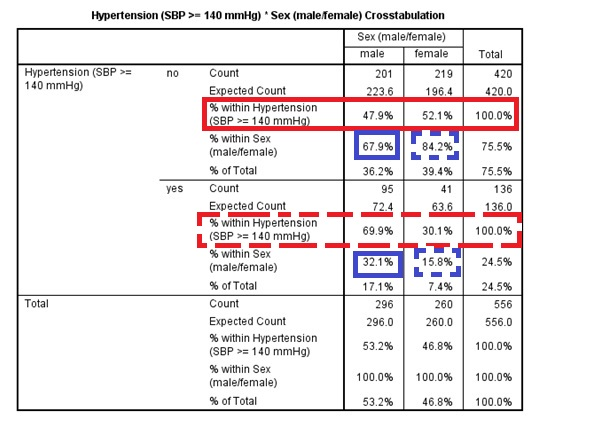
\includegraphics{C:/OneDrive - University of Leeds/Teaching/MSc IH/YCHI5045M/Teaching materials/Computer sessions/YCHI5045M practical sessions website/Images/Chi-square table.jpg}

Because of the way the table is laid out (with sex along the top and htn down the side) it makes most sense to look at the results from the ``point of view'' of the htn variable, looking at the relative frequency of men and women for each level of htn. So to do this with the above table we are looking across the rows at the ``\% within Hypertension\ldots{}'' values. First look at the row outlined in solid red for htn = no. This tells us that out of the individuals who were htn = no 47.9\% were men and 52.1\% were women. Next look at the row outlined in dashed red for htn = yes. This tells us that out of the individuals who were htn = yes 69.9\% were men and 30.1\% were women. Therefore, there appears to be a strong association between hypertension status and sex, with men being more likely to be hypertensive than women, i.e.~as we ``move'' from one level of htn to the other the relative frequency of sex varies substantially from roughly 50\%:50\% to roughly 70\%:30\%. We can also look at these results from the ``point of view'' of the sex variable, but now because of the way the table is laid out it makes more sense to look down the sex level columns or reproduce the table with the variables the other way around. Look at the values outlined in solid blue in the male column. These show us that of the individuals who were men 67.9\% were not hypertensive and 32.1\% were. Finally look at the values outlined in dashed blue in the female column. These show us that of the individuals who were female 84.2\% were not hypertensive and 15.8\% were. So again it indicates the same direction and strength of association, because it's the same data, but looking from ``the point of view'' of the other variable. I find looking from the ``point of view'' of the assumed outcome variable more logical and intuitive (i.e.~the first ``view'') because it's the assume causal relationship, but you may disagree.

Lastly we come to the fourth table ``Symmetric Measures''. This presents the Phi and Cramer's V statistics and their associated p-values. The statistics both measure the strength of the association between the two variables in the analysis, and both go from 0 (no association) to 1 (``perfectly'' associated). The associated p-value shows you, assuming the Phi/Cramer's V value is 0, how likely you were to observe a value at least as great as the one observed due to sampling error alone. These statistics can help you interpret how strong any association is, but they are difficult to interpret. When both variables have two levels then they are equivalent in interpretation to a linear correlation coefficient with a simple and useful interpretation (the strength of association on a 0-1 or 0-100\% scale), but when there are more than two levels in one or both variables there's no clear intuitive interpretation!

Therefore, I would recommend firstly looking at the p-value to see if there is any reasonable evidence for an overall association between your two categorical variables (i.e.~based on the standard P ≤ 0.05 threshold), and the looking at the relative frequencies (\% of observations within different levels of one variable for each level of the other) as we have done above to judge where any associations might exist, in what direction and how strong they appear to be.

\hypertarget{step-4-report-and-interpret-the-results-1}{%
\section{Step 4: report and interpret the results}\label{step-4-report-and-interpret-the-results-1}}

In our methods section we would explain that we used a chi-square test of independence and justify why we did so. Then in a results section we could say something like:

\begin{quote}
Among males 67.9\% (201/296) of individuals had hypertension (systolic blood pressure ≥140 mmHg) while among females 84.2\% (219/260) of individuals had hypertension. A chi-square test of independence showed that this represented a statistically significant association between hypertension and sex (P\textless0.001).
\end{quote}

This allows readers to understand the direction and possible size of associations between the relative outcome frequencies in each of the independent variable groups, and the associated inferential hypothesis test p-value result, which loosely speaking gives us a sense of how confident we can be in concluding that the exact observed association in the sample represents the association that exists in the target population.

\hypertarget{limitations-3}{%
\section{Limitations}\label{limitations-3}}

The main limitation of the chi-square test of independence is that we do not get any confidence intervals on our raw measures of effect size: the relative frequencies (i.e.~the raw measure of the direction and strength of the association). We only get an overall p-value that tells us, assuming there is no association between the two categorical variables, how likely we are to have observed an association (in either direction) at least as great as the one we have observed due to sampling error alone. So all it can indicate is if there is likely to be an overall association between the two variables given the uncertainty in the data. It tells us nothing about the direction or size of any association, or which levels it involves.

When both variables have two levels, like with our example, we know any association must be between both levels of each variable. However, when there are more than two levels in one or both variables it's even less clear. For example, assume we looked at the association between the htn and ses variables. If we found the p-value for a chi-square test of independence was \textless{} 0.05 we could conclude there was evidence for an overall association. However, we could get a significant p-value if the relative frequency of hypertension was similar for two levels of ses and only differed for the remaining level, or we could get a significant p-value if the relative frequency of hypertension was different among all three levels of ses. Therefore, all we can do is conclude whether there is evidence for an overall association based on the p-value, and then cautiously interpret the relative frequencies (measures of effect) to see which levels, what direction and what size of associations appear to exist. As you can see this is much, much less robust and satisfactory than having confidence intervals for our raw measures of effect size.

\hypertarget{expected-cell-counts-5}{%
\section{Expected cell counts \textless5}\label{expected-cell-counts-5}}

What if one or more of our expected cell counts are \textless5? Then we can use a similar test that can deal with this problem (but is typically less powerful when it's not an issue) called the Fisher's Exact test. To include this test in our chi-square results table when we go to the Crosstabs tool add in the variables as above but now click the Exact button and then tick the Exact button (you can leave the Time limit per test as it is). Then click OK and in the Chi-Square Tests table you will see an additional row called Fisher's Exact Test. Again all we get is a two-sided p-value (``Exact Sig. (2-sided)'') based on the test statistic (``Value'') given the degrees of freedom (``df''), which as always just tells us, assuming the null hypothesis is true, how likely we were to have observed data reflecting a relationship that differed from the null hypothesis at least as greatly as that observed.

\hypertarget{exercise-chi-square-test-of-independence}{%
\section{Exercise: chi-square test of independence}\label{exercise-chi-square-test-of-independence}}

Using the ``SBP final data.sav'' dataset and via the process outlined above use a chi-square test of independence to analyse the relationship between BMI and ACE inhibitor usage during the past three months, with the hypothetical research question being is BMI related to ACE inhibitor usage?

\begin{itemize}
\item
  First convert the BMI variable into a binary variable based on BMI values \textless30 kg/m² and those ≥ 30 kg/m².
\item
  Run the chi-square test of independence using the new categorical variable BMI (\textless30 kg/m² or ≥ 30 kg/m²) and ace.
\item
  Hint: enter your new categorical BMI variable into the Row(s): box in the Crosstabs tool and then in the Crosstabulation table look across the top and bottom halves of the table. For example, the top half of the table will, depending on how you've coded your BMI categorical variable, include the count (frequency) and \% of individuals who reported (yes) and did not report (no) using ACE inhibitors during the past month within the relevant BMI group. You can then compare the frequency and \% of individuals reporting usage between the two BMI groups, along with the chi-square p-value result in the following table.
\item
  In the YCHI5045M computer sessions materials ``Exercises'' folder open the ``Exercises.docx'' Word document and scroll down to \textbf{Chi-square test of independence: the relationship between BMI and ACE inhibitor usage}.
\item
  Write a couple of sentences reporting the results of your analysis. Include the basic descriptive statistics: overall sample size and frequency and proportion/percentage of individuals with low and high BMI who reported using ACE inhibitors during the past three months. Also be sure to include sufficient details about the type of analysis used, and of course the key inferential result. Round results to one decimal place. You don't need to explain anything about the study or interpret the clinical or practical importance of the result.
\item
  Write a sentence or two about the key limitations of this analysis \emph{in terms of interpreting the result}.
\item
  Once you've completed this compare your reporting to the below example text.
\end{itemize}

\textbf{Example results reporting text}

I analysed the relationship between BMI, defined/grouped as \textless30 kg/m² or ≥30 kg/m², and ACE inhibitor usage during the past three months. Out of a total sample size of 529 individuals, among individuals with reported BMI values \textless30 kg/m² 4.7\% (20/429) reported using ACE inhibitors during the past three months while among individuals with reported BMI values ≥ 30 kg/m² 7\% (7/100) reported using ACE inhibitors during the past three months, but this difference was not statistically significant (P = 0.3) based on a chi-square test of independence. Therefore, there was no clear evidence for a relationship between BMI when grouped as \textless30 kg/m² or ≥30 kg/m² and ACE inhibitor usage frequency during the past three months in this target population. However, the key limitation of this analysis is that it does not adjust for any other confounding variables, of which there are likely to be many (especially in an observational cross-sectional study like this). Therefore, this is likely to represent a biased estimate of the independent relationship between BMI (as defined/grouped here) and ACE inhibitor usage within the past three months in this target population.

\hypertarget{the-chi-square-goodness-of-fit-test}{%
\chapter{The chi-square goodness-of-fit test}\label{the-chi-square-goodness-of-fit-test}}

There is another chi-square based test usually called the chi-square goodness-of-fit test. We will not practice this test here as it's far less commonly required/used than the chi-square independence test. In brief though, the chi-square goodness-of-fit test is a nonparametric test for single variables that is used to analyse whether the distribution of cases (units of observation) in a single categorical variable follows a known or hypothesised distribution. For example, whether the proportion of males and females in a sample follows the distribution of males and females in a given target population, or a distribution that is ``hypothesised'', such as the proportion of males compared to females that we expect to have a certain characteristic/disease etc.

A good overview of the test with instructions of how to use it in SPSS can be found here: \url{https://statistics.laerd.com/spss-tutorials/chi-square-goodness-of-fit-test-in-spss-statistics.php}

\hypertarget{mcnemars-test}{%
\chapter{McNemar's test}\label{mcnemars-test}}

Like with the paired t-test there is an alternative to the chi-square test of independence for the situation where you want to compare a binary outcome between two groups (i.e.~an independent variable with two levels) but where those two groups are paired. This test is known as McNemar's test. A typical scenario where this test might be applicable is where you have a binary outcome, e.g.~a covid test (positive/negative), with the outcome measured/recorded from the same set of individuals at two points in time, e.g.~before/after an intervention. We will not look further at this test or practice its use in this course, but a good overview of the test with instructions of how to use it in SPSS can be found here:

\url{https://statistics.laerd.com/spss-tutorials/mcnemars-test-using-spss-statistics.php}

\hypertarget{multiple-linear-regression}{%
\chapter{Multiple linear regression}\label{multiple-linear-regression}}

\hypertarget{key-terminology-and-concepts}{%
\section{Key terminology and concepts}\label{key-terminology-and-concepts}}

If necessary please read the below guide to key terminology and concepts before reading further as we will be using these terms when discussing linear regression and the modelling process in SPSS without further explanation.

\begin{itemize}
\item
  \textbf{Model} = Loosely speaking the outcome variable and the set of independent variables that you are analysing via linear regression, plus their functional form (see below). Note: although simpler analyses like the independent t-test are referred to as ``statistical tests'', creating the false illusion of a fundamental difference from regression ``modelling'', they have the same underlying mathematical form. Simply put, parameteric statistical tests like the independent t-test are models too.
\item
  \textbf{Functional form/model parameterisation} = In what mathematical form you add independent variables to your model. Practically speaking this is whether your model assumes 1) a simple linear relationship between a given independent variable and the outcome (also called a ``main effect''), or 2) an interaction between a given independent variable and one or more other independent variables and the outcome, or 3) a non-linear relationship between a given independent variable and the outcome (although many other functional forms are possible).
\item
  \textbf{Model building} = The process by which you decide which independent variables to include in your model.
\item
  \textbf{Coefficient or parameter or (model) term} = The point estimate measuring/indicating the direction and size of the relationship between a given independent variable and the outcome that your linear regression estimates.
\item
  \textbf{Focal relationship} = A relationship between a given independent variable and an outcome that is the focus of the analysis and research question, such as the effect of smoking status on systolic blood pressure.
\item
  \textbf{Confounder or confounding variable} = With respect to a focal relationship, say the effect of smoking status on systolic blood pressure, a confounder or confounding variable is a ``common cause'' of both the independent variable of interest (smoking status) and the outcome (systolic blood pressure). For this example a plausible confounder might be ``stress level'', because it's very plausible that stress can induce people to take up smoking or restart smoking and that stress can increase blood pressure on its own.
\item
  \textbf{Competing exposure} = With respect to a focal relationship, say the effect of smoking status on systolic blood pressure, a competing exposure is a cause of the outcome but is not caused by the independent variable of interest and does not cause the independent variable of interest. For this example a plausible competing exposure might be the presence of a certain gene that predisposes individuals to high blood pressure, whilst having no effect on their likelihood of taking up smoking or remaining a smoker, because it would, on average, lead to higher blood pressure in individuals but not affect their likelihood of smoking.
\item
  \textbf{Sufficient adjustment set} = With respect to a focal relationship, say the effect of smoking status on systolic blood pressure, a sufficient adjustment set is a set of variables that, if fully ``conditioned on'' (i.e.~adjusted for by including in a regression model), will provide an unbiased estimate for the causal effect of the independent variable of interest by adjusting for all sources of confounding.
\end{itemize}

\hypertarget{overview-with-a-focus-on-causal-inference-from-observational-data}{%
\section{Overview with a focus on causal inference from observational data}\label{overview-with-a-focus-on-causal-inference-from-observational-data}}

Multiple linear regression is used to analyse the relationship(s) between one numerical outcome variable and one or more independent variables that can be numerical or categorical or a mixture of both. When you have one numerical outcome and one numerical or categorical independent variable this is sometimes referred to as ``simple linear regression'', but there's no qualitative difference from multiple linear regression, and we'll often just refer to ``linear regression'' from here on. Note: when we have one outcome variable and multiple independent variables it is a multiple linear regression not a multivariate linear regression. Multivariate refers to analyses of more than one outcome variable.

Linear regression modelling is therefore an extremely flexible and powerful method of analysis. Linear regression models are used for a variety of purposes, but primarily they are used for prediction and causal inference. Prediction models (actually more often using logistic regression) are typically used for diagnosis or prognosis, and are usually developed using more or less ``theory free'' and automated methods, where data are primarily used to build the model. However, most research in the health sciences focuses on attempting to understand causes of outcomes, such as does smoking cause lung cancer? This has historically been what ``statistical inference'' tended to mean, at least in practice. In the context of robust randomised controlled trials it is generally accepted that causal effects can be clearly identified, and you can certainly use regression models to this as appropriate to the data. However, in the context of observational studies it is generally accepted to be much more challenging to clearly identify causal effects, primarily due to the challenges of accurately modelling the processes generating your outcome of interest and avoiding various source of bias such as confounding and other less well known biases.

Broadly speaking, in the context of observational studies the historical, and still dominant, approach to trying to understand causal effects has been the following: 1) collect some data on an outcome of interest and a range of independent variables thought to be possible causes or confounders, 2) use a mix of theory and data-driven choices to build a regression model that is the ``best'' in some sense, usually at minimising the unexplained variation in the outcome, and 3) interpret all the independent variables as causal effects in relation to the outcome, at least implicitly. I say implicitly because the typical approach in research using observational studies, given the limitations of observational designs at robustly and clearly identifying causal effects, has been to refer to the relationships identified between independent variables and outcomes as ``associations'' or another similar term. In such studies researchers usually also state that causation cannot be inferred from the study given its limitations, but then in practice still treat the identified relationships as causal, which is clearly not a very satisfactory approach!

For a while now though a field know as ``causal inference'' has been developing and promoting methods for less biased analysis of causal research questions in observational studies, as it has become increasingly clear that existing methods and approaches have some substantial (and often hidden and/or counterintuitive) biases. Most of the learning and approaches from this field area beyond the scope of this introductory course, but we will try and incorporate some of the key ideas and findings below, while acknowledging the gaps.

Very simply speaking, particularly in the context of observational studies, research has shown that data-driven automated model selection processes typically lead to biased models that cannot identify and accurately estimate causal relationships, while also producing inferential results that have falsely inflated precision and power. Research has also shown that it is typically not valid to interpret the results of a regression model in terms of \emph{all the independent variables} in the model reflecting causal relationships. This is known as the ``Table 2 fallacy''.

Instead, within a given study every focal relationship of interest, say the relationship between stress and blood pressure, should be analysed using a separate model containing its own set of independent variables (other than the independent variable of focal interest), which may or may not differ from the set of independent variables used when analysing a different focal relationship of interest within the data, say the relationship between BMI and blood pressure. Broadly speaking, each model for every separate focal relationship of interest should contain a ``sufficient adjustment set'' of independent variables that suitably adjust for \emph{all key sources of confounding of that relationship}, and this set of variables should be chosen based on theory and plausible/sensible decisions, not via a data-driven automated process.

In this practical and course we will not go further into these aspects of causal inference, and please be clear that this is just a very simplistic overview of a few of the key principles of causal inference as it relates to analysing observational data using regression models, but there is much more to learn and many details are not covered! However, we will take some of these key principles forward. Specifically, for this linear regression and the following logistic regression practical sessions we will assume we are aiming to make causal inferences about the likely causes of variation in systolic blood pressure and hypertension status respectively using the SBP data, which we assume to have come from an observational study (specifically a cross-sectional design). We will be interested in the assumed causal effects of all the available independent variables. We will not use any form of data-driven automated process when building our model, but we will select a single set of independent variables that we assume represents the sufficient adjustment set of variables for each variable in that set. That is, we will interpret the relationship of each independent variable in our single model as though it was an estimate of a possible causal effect between itself and the outcome based on a single model, i.e.~we will assume that every independent variable in our model is a focal relationship of interest. However, please bear in mind that while this practice is extremely common in the scientific literature, as discussed above in practice this would almost certainly be committing the ``Table 2 fallacy'', and it's just for the purposes of keeping things simple that we won't try and create sufficient adjustment sets for every focal relationship.

\hypertarget{causal-inference-references}{%
\subsection{Causal inference references}\label{causal-inference-references}}

If you are likely to carry out quantitative research in your dissertation and/or later career I would strongly advise that as well as putting time and effort into learning statistics, i.e.~analysing data, that you put time and effort into learning about causal inference and put into practice as many of the recommended approaches as you can. Although it's still somewhat of an emerging field learning from it is being adopted rapidly by epidemiology and the health sciences, and understanding at least the basic principles and key recommendations will really benefit your research and expertise.

Some very useful causal inference references are:

\textbf{Hernan and Robins' causal inference book.} This is an excellent and comprehensive book. It gets quite technical in places but there's not necessarily a way to simplify things further. If you want to do robust causal inference it's not a simple or easy thing unfortunately.

\begin{itemize}
\tightlist
\item
  \url{https://www.hsph.harvard.edu/miguel-hernan/causal-inference-book/}
\end{itemize}

\textbf{Free online course about using directed acyclic diagrams (DAGs) to select variables for models.} DAGs are a brilliant and relatively easy to use tool for thinking through what independent variables constitute a sufficient adjustment set for a given focal relationship when planning an analysis of data relating to that focal relationship. They are highly recommended by causal inference practitioners, and are literally just diagrams - no maths involved.

\url{https://www.edx.org/course/causal-diagrams-draw-your-assumptions-before-your}

\textbf{Table 2 fallacy paper.}

\begin{itemize}
\tightlist
\item
  \url{https://academic.oup.com/aje/article/177/4/292/147738}
\end{itemize}

\textbf{Why step-wise selection methods commonly used to build regression models are bad.}

\begin{itemize}
\tightlist
\item
  \url{https://towardsdatascience.com/stopping-stepwise-why-stepwise-selection-is-bad-and-what-you-should-use-instead-90818b3f52df}
\end{itemize}

\hypertarget{interactions-and-non-linear-relationships}{%
\subsection{Interactions and non-linear relationships}\label{interactions-and-non-linear-relationships}}

Linear regression can also be used to look at interactions between different variables (e.g.~how the relationship between smoking status and systolic blood pressure changes based on sex), and to model non-linear relationships (e.g.~the relationship between age and blood pressure, which is typically fairly flat at young ages and then increases through middle age before flattening out). In practice most processes/phenomena interact and are non-linear to a greater or less extent, but it is often a reasonable simplifying assumption to treat variables as independent (non-interacting) and relationships as linear, unless the interactions and/or non-linear relationships are clearly strong or a key part of your research question. Therefore, as these issues are complicated and often not required when analysing maybe most data simple datasets we will not look at or practice the techniques needed to model interactions and non-linear relationships.

Note: the ``linear'' part of linear regression refers to the fact that in the linear regression model the coefficients or parameters are ``linear'', i.e.~the model is just a simple sum of those coefficients:

\begin{quote}
y = α + β1X1 + β2X2 + \ldots{} + βnXn
\end{quote}

Where y is the model predicted outcome value, α is the intercept, the βs are the independent variable coefficients and the Xs are the independent variable values.

\hypertarget{scenario-11}{%
\section{Scenario}\label{scenario-11}}

We wish to understand all the main likely causes of variation in individuals' systolic blood pressure using the data collected in the SBP final dataset. We'll use a linear regression model/analysis to look at this question. Refer to the ``The datasets'' section within the ``Introduction to SPSS'' section for full details if you need a full reminder, but briefly this dataset contains data on 556 individuals who were (hypothetically speaking!) sampled in a cross-sectional survey, and had data collected on their systolic blood pressure plus certain socio-demographic (age, sex, socio-economic status) and health characteristics (BMI, salt intake and ACE inhibitor usage).

As discussed above we will assume, based on existing theory/evidence and plausible, critical thinking, that all our measured independent variables are all likely causes of variation in systolic blood pressure and collectively simultaneously act as a sufficient adjustment set when interpreting each independent variable's relationship with the outcome causally. That is, we will just create one linear regression model containing all the independent variables and assume that this model represents the same sufficient adjustment set for each independent variable (i.e.~when interpreting the effect of each independent variable causally we will assume all other variables in the model are confounders of that relationship that require adjusting for to obtain an unbiased estimate of the focal causal effect). In reality if we were doing this we should start by deciding which focal relationships of interest we were interested in, which may well not be all of our collected independent variables, and for each focal relationship of interest we should define a sufficient adjustment set which may well differ from the sufficient adjustment set of other focal relationships of interest. This would typically be a big and time consuming process requiring a lot of careful critical thought and research/subject matter knowledge.

\begin{itemize}
\tightlist
\item
  Load the ``SBP data final.sav'' dataset.
\end{itemize}

\hypertarget{step-1-explore-the-data}{%
\section{Step 1: explore the data}\label{step-1-explore-the-data}}

\href{https://youtu.be/aZpnd63IM4s}{Video instructions: explore the data for a linear regression}

\textbf{Written instructions: explore the data for a linear regression}

Although we are not taking a data-driven approach to model building, which often involves extensive exploration of patterns in your dataset to largely/wholly determine your model building along with automated model selection processes, it is always advisable to conduct some focused exploration of your dataset to understand the data and the guide certain decisions in your model building process. Note: this would follow your data preparation stage, where you would already have a good sense of the key characteristics of each variable, such as the type of data it contains, the range of values present etc.

Specifically, although you should not typically use your dataset to guide which independent variables are included in your model (and as discussed earlier for any given focal relationship that should be based on theory and plausible hypotheses about what constitutes a sufficient adjustment set), most researchers would recommend thoroughly exploring you data in terms of: 1) the distribution of your outcome and independent variables, to ensure you understand them well and are taking a suitable modelling approach (e.g.~linear regression rather than another type of regression), and 2) what functional form of model makes good sense given the relationships between your independent and outcome variables, primarily whether there are any clear/strong non-linear relationships or interactions, although we will not look at exploring interactions in this practical as they are beyond the scope of this course.

\hypertarget{univariate-exploration}{%
\subsection{Univariate exploration}\label{univariate-exploration}}

To understand the distribution of your variables you can use histograms for numerical variables and bar charts for categorical variables. Let's run a histogram for our outcome variable.

\begin{itemize}
\tightlist
\item
  From the main menu go: Graphs \textgreater{} Legacy Dialogues \textgreater{} Histograms. Add sbp into the Variable: box, tick the Display normal curve box and click OK. What do you see?
\end{itemize}

What does the distribution of the outcome look like?

There appears to be a slightly odd ``gap'' near the mean, but overall the variable appears to pretty closely follow a normal distribution.

Next let's look at a bar chart for our ses variable.

\begin{itemize}
\tightlist
\item
  From the main menu go: Graphs \textgreater{} Legacy Dialogues \textgreater{} Bar. Then click the Simple option and Define. Add ses to the Category axis: box, tick the \% of cases option and click OK. What do you see?
\end{itemize}

What does the distribution of the socio-economic status variable look like?

Most participants were of low socio-economic status, with successively smaller proportions being of medium and high socio-economic status.

You can use these two types of graphs to explore the distribution of all the variables. In a real analysis you would certainly want to do this, but for the sake of time you may want to move on now that you know how to do this.

\hypertarget{bivariate-exploration}{%
\subsection{Bivariate exploration}\label{bivariate-exploration}}

\hypertarget{numerical-independent-variables}{%
\subsubsection{Numerical independent variables}\label{numerical-independent-variables}}

First let's look at relationships between the outcome and numerical variables (i.e.~bivariate relationships) to understand whether it's reasonable to assume simple linear relationships for your numerical independent variables or whether any need to be modelled via the addition of non-linear terms to the model. We'll just look at age and we'll use a scatterplot.

\begin{itemize}
\tightlist
\item
  From the main menu go: Graphs \textgreater{} Legacy Dialogues \textgreater{} Scatter/Dot. Then select the Simple option and click Define. Add the sbp variable into the Y Axis: box and age into the X Axis: box then click OK. What do you see?
\end{itemize}

What does the relationship between age and systolic blood pressure look like?

It's hard to say much other than there's no clearly strong linear or non-linear relationship. However, this is a good example of why you can't always interpret bivariate graphs very easily, because when there is a lot of variation in the data it can easily hide weaker relationships, because as we'll see later there is evidence of a relationship here.

What if we had seen a clear non-linear relationship? There are two main options within a regression modelling framework:

\begin{enumerate}
\def\labelenumi{\arabic{enumi}.}
\item
  Convert your numerical independent variable into a categorical variable.
\item
  Include additional ``polynomial'' terms of the relevant independent variable. This just means that as well as including, say, age in the model you include age² or possibly higher-order terms as well.
\end{enumerate}

Option 1 is often the best choice because although it might not model the relationship as well as option 2 it provides results that are easier to interpret. If you ever need to do this as always you should think carefully and critically about what cut-points to use when converting your numerical variable to a categorical variable. There aren't necessarily clear ``rules'' about this, but within the framework we've discussed it would be most consistent to choose cut-points based on theory rather than driven by what the sample data suggest are key cut-points.

\hypertarget{categorical-independent-variables}{%
\subsubsection{Categorical independent variables}\label{categorical-independent-variables}}

Now let's look at the relationship between categorical variables and the numerical outcome. To do this we can use bar charts or boxplots. Boxplots are probably better as they provide more information within the plot, although you can present much of the same information on a barchart if you know how using statistical software like R. Why would we want to do this, given you cannot have a non-linear relationship between a categorical variable and a numerical outcome? The main reason would be to inform us whether any levels within categorical variables might be suitable for merging/pooling together if necessary, and to understand whether the variance within category levels is approximately equal, which is a key assumption of linear regression.

\begin{itemize}
\tightlist
\item
  Look at the figure below to understand how to interpret boxplots:
\end{itemize}

\begin{figure}
\centering
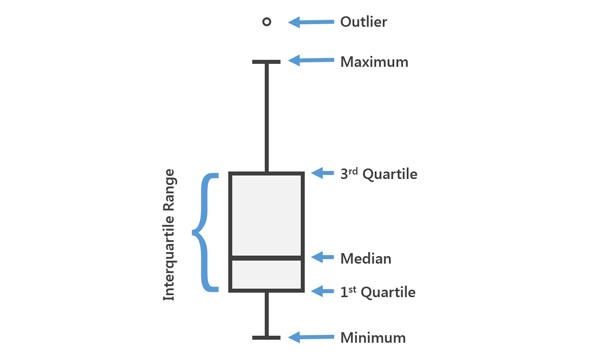
\includegraphics{C:/OneDrive - University of Leeds/Teaching/MSc IH/YCHI5045M/Teaching materials/Computer sessions/YCHI5045M practical sessions website/Images/Boxplot.jpg}
\caption{Boxplot explained}
\end{figure}

Let's look at the relationship between the outcome and the categorical variable sex with a boxplot:

\begin{itemize}
\tightlist
\item
  From the main menu go: Graphs \textgreater{} Legacy Dialogues \textgreater{} Boxplot, then select Simple and click Define. Add the sbp variable into the Variable: box and sex into the Category Axis: box and click OK. What do you see?
\end{itemize}

What does the relationship between sex and systolic blood pressure look like?

In our sample males clearly tend to have moderately higher values of SBP than females on average, but both sexes have a broadly similar spread (i.e.~approximately equal variance) of SBP values. We can also see that systolic blood pressure values in both groups appear to follow a fairly normal distribution, which you can tell this by the fact that the box plots are quite symmetrical, unlike the explanatory boxplot image above where the data would clearly be right skewed due to the larger spread of higher values. Asymmetry indicates a non-normal, skewed distribution with a higher spread of observations indicating right-skew and a lower spread of observations indicating left skew. You can always plot a histogram of the outcome within each group to understand this more clearly.

Again, you can now use these two types of plots to explore the relationships between all the other independent variables and the outcome if you wish, but there's no real need to do this for this practical so feel free to move on.

\hypertarget{step-2-run-the-linear-regression-model}{%
\section{Step 2: run the linear regression model}\label{step-2-run-the-linear-regression-model}}

\href{https://youtu.be/gQRLkJNO0R0}{Video instructions: run the linear regression model}

\textbf{Written instructions: run the linear regression model}

Remember linear regression allows you to look at relationships between a numerical outcome variable and any number of numerical or categorical independent variables, assuming all the assumptions of the method are met (we'll check these out shortly). So let's see how we build, run and estimate our linear regression model in SPSS.

\begin{itemize}
\item
  From the main menu go: Analyze \textgreater{} General Linear Model \textgreater{} Univariate. Note: a univariate general linear model is essentially another name (less commonly used) for (multiple) linear regression, although confusingly SPSS also has various ``regression'' modelling tools as well that produce different linear regression model but with slightly different options available or (somewhat pointless) restrictions compared to this tool. One of the main benefit of the General Linear Model - Univariate tool is that you can add categorical variables without first converting them to dummy variables (see later for an explanation of what this means).
\item
  Next in the Univariate tool we add our outcome variable sbp to the Dependent Variable: box. Then we add our independent variables. SPSS has separate boxes for numerical and categorical independent variables, so we add our numerical variables (bmi, salt and age) into the Covariate(s): box (you can highlight them all -- hold shift while left-clicking -- and add them together), and our categorical variables (sex, ses and ace) into the Fixed Factor(s): box (a factor is another term for a categorical variable). We can ignore the Random Factor(s): box and WLS Weight: box (see the help if you want to understand what they are for).
\end{itemize}

Next we need to edit a number of options. Most importantly we need to specify the ``functional form'' of our model or how the model is ``parameterised''. Essentially we can either add all variables as simple ``main effects'', which means the independent linear effect of each variable is estimated, or we can add additional terms to create interactions between two or more variables, and/or we can add non-linear terms for one or more variables. However, as interactions and non-linear terms are beyond the scope of this course we will just assume all our variables have simple linear relationships with our outcome.

\begin{itemize}
\item
  Therefore, click on the Model tool button, then under Specify Model select the Custom option, then select all variables in the Factors \& Covariates: box (to do this click on the top variable, then click and hold shift before clicking on the bottom most variable). Next (with all variables still selected) under the Specify Model section click the Build terms button, then under the Build Terms(s) Type: section click on the drop-down menu and change it to Main effects. This is where you could create interaction terms between two or more terms/variables in the model if you wished, but we'll just stick with main effects. Therefore, now click the right facing arrow beneath this menu which will add all selected variables as main effects terms into the Model: box. Ensure that the Include intercept in model box is ticked and click OK.
\item
  Next click the Save button and under Predicted Values tick the Unstandardized box, and then under Residuals tick the Unstandardized box, and then under Diagnostics tick the box for Cook's distance. This tells SPSS to save the unstandardised predictions and residuals, and values for ``Cook's distance''. We will explain these later.
\item
  Lastly click the Options button, and then under Display tick the Parameter estimates box and click Continue and then OK. The output window will then pop up with the results, but first\ldots{}
\end{itemize}

\hypertarget{step-3-check-the-assumptions-of-linear-regression}{%
\section{Step 3: check the assumptions of linear regression}\label{step-3-check-the-assumptions-of-linear-regression}}

Before we look at the results that appear in the output window we must first check whether we can treat the results as robust and valid. Our results are only valid if the assumptions of the linear regression model have been met/hold, i.e.~if they have not been violated. Below we'll go through the assumptions and how to check them, which is more complicated than for the simpler statistical tests we ran previously.

\textbf{1. Continuous outcome}

Theoretically the outcome variable must be continuous, but like with t-tests this can be relaxed and you can safely use linear regression for discrete outcome variables as long as the other assumptions hold.

\textbf{2. Independent observations}

Technically this means that the residuals or model errors (variation not explained by the model) of one observation should not be correlated/related (be able to predict) to the residuals of other observations. As with the t-tests you should be able to understand from your study design whether you have independent observations or not. There are two main reasons for non-independent observations. 1) You have outcome measurements on your units of observation at more than one point in time (repeated measures) that are all included in the outcome variable. 2) You have outcome measurements on your units of observation that are nested within a larger cluster, such as patients within facilities, where patients from the same facility are going to be more similar and have correlated outcomes compared to patients from different facilities. We know our study design (simple random sampling of participants) ensures our observations are independent, so we don't need to worry about this assumption further. What if your data are not independent? See below.

\textbf{Dealing with non-independent observations in linear regression modelling}

There are sophisticated and powerful ways of dealing with problems of non-independence, but we don't go into them here. However, a simple solution for non-independent observations due to having multiple measurements across time is to just use observations from one time point only as your outcome (if this makes sense), or to take the average across all time points (if this makes sense), or to take the difference between your first and last time points and use these change scores as your new outcome (if this makes sense). And a simple solution for having non-independent observations due to clustering is to calculate summary values of the outcome based on all observations within each cluster. For example, if your outcome is a numerical variable, such as SBP, and you are looking at patients within facilities, then you can calculate the mean SBP across all patients in each facility, and then use the facility-level mean SBP as your outcome. For binary categorical variables (e.g.~hypertension -- yes/no) you can select one level (e.g.~hypertension = yes) and calculate the proportion or percentage of observations in that level per cluster. For categorical variables with \textgreater2 levels you have to create separate summary percentage variables for each level.

\textbf{3. Normally distributed residuals}

Remember that in linear regression the residuals or model errors are simply the differences between each observed outcome value and the model predicted value (based on the linear regression equation). Technically the assumption here is ``multivariate normality of residuals or errors''. In practical terms this just means checking that the residuals are (approximately) normally distributed, which luckily is easy to do. Linear regression assumes normally distributed errors, and if this assumption is violated then the resulting confidence intervals and p-values for coefficients can be biased (usually too narrow and too small respectively).

When we ran our linear regression using the General Linear Model -- Univariate tool we told SPSS to calculate the ``unstandardised'' residuals for each observation and save them as a new variable, which SPSS will have called RES\_1. To check whether the residuals are approximately normally distributed we could use a statistical test, but again this is sensitive to sample size and even if violated doesn't necessarily mean our results won't be robust, so it's best to use a histogram.

\begin{itemize}
\tightlist
\item
  From the main menu go: Graphs \textgreater{} Legacy Dialogues \textgreater{} Histogram. Then add the RES\_1 variable into the Variable: box, tick the Display normal curve box and click OK. What can you conclude?
\end{itemize}

\textbf{How are the residuals distributed?}

The residuals appear to be reasonably approximately normal so we can safely assume this assumption has not been violated in our model. If the residuals were not approximately normally distributed then we can try to transform the outcome to increase the normality of their distribution. You can use the same methods as discussed and practiced in the ``Inferential analysis 2: the independent t-test applied to a skewed outcome'' practical, specifically see the ``Step 2: transform the outcome'' section.

\textbf{4. Linearity of the relationships between the residuals and all numerical variables}

Although you should have already confirmed the nature of the bivariate relationships between sbp and the numerical independent variables during your pre-modelling data exploration phase, once we are dealing with a multiple linear regression model it can be the case that once you adjust for a certain variable the adjusted relationship between another numerical independent variable and the outcome becomes non-linear. If this is the case the un-modelled non-linearity will be reflected in the residuals and cause bias in the inferential results (confidence intervals and p-values). Therefore, we must check whether the residuals show any non-linear patterns (curved trends) when plotted against the values of each independent numerical variable.

\begin{itemize}
\tightlist
\item
  We will use a scatterplot. From the main menu: Graphs \textgreater{} Legacy Dialogues \textgreater{} Scatter/Dot. Then select Simple Scatter and click Define. Add the RES\_1 variable into the Y Axis: box and the age variable into the X Axis: box and click OK. What do you see?
\end{itemize}

What is the relationship between the residuals and age?

There is no clear non-linear trend as the residuals are scattered fairly evenly and linearly across values of age.

In a real data analysis you should repeat this process for the other numerical independent variables in the model, but feel free to move on now if you wish because there are also no issues with the remaining variables. If you had found any non-linear relationships involving numerical independent variables then see the above ``Bivariate exploration'' section for a discussion of some possible solutions.

\textbf{5. Homoscedasticity: constant variance of the residuals across model predicted values}

The technical name for this assumption is homoscedasticity, but in practical terms this just means that there should be no systematic pattern or change in the amount of variation (i.e.~spread) in the residuals across the model predicted values (also called the model fitted values). If the residual variance changes with predicted values (most commonly increasing at higher predicted values) then this is known as heteroscedasticity, and this can again lead to confidence intervals and p-values for coefficients can be biased (usually too narrow and too small respectively). Again there are statistical tests available to ``test'' for this, but we will use graphical methods. Again this is very easy to check: we just plot the model predicted values against the model residuals and hope to see ``random noise''.

See the following three figures for an illustration of some examples of clear heteroscedasticity and homoscedasticity:

\begin{figure}
\centering
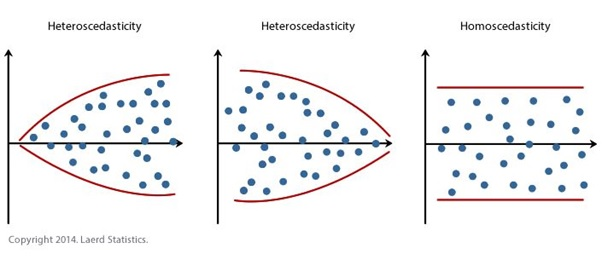
\includegraphics{C:/OneDrive - University of Leeds/Teaching/MSc IH/YCHI5045M/Teaching materials/Computer sessions/YCHI5045M practical sessions website/Images/hetero-homo-scedasticity.jpg}
\caption{Illustrations of idealised heteroscedasticity and homoscedasticity residual patterns}
\end{figure}

Note: these are in an idealised/very clear form. You will often see some tapering of points at either end of the main spread of points because there is usually less data at these places, but this is not usually something to worry about.

Let's now produce the necessary plot and check for violation of this assumption:

\begin{itemize}
\tightlist
\item
  From the main menu go: Graphs \textgreater{} Legacy \textgreater{} Scatter/Dot, then select Simple Scatter and click Define. Add the RES\_1 variable into the Y Axis: box and the PRE\_1 variable into the X Axis: box and click OK. Note: you can also get SPSS to make this graph via the Options menu in the General Linear Model Univariate tool, but it is a lot smaller and harder to see when made that way. What can we conclude?
\end{itemize}

\textbf{Is the homoscedasticity assumption violated or not?}

The spread of the residuals looks fairly even across all values of the model predictions for the outcome, so we can safely assume this assumption has not been violated.

What if there had been a clear pattern in the residuals when plotted against the model predicted values?

\textbf{How to deal with heteroscedasticity}

The first thing to do would be to try and find out why this was. This is usually either caused by 1) having an outcome that covers a very large range of values, because typically the variance will be greater at larger values, even if the model is correctly specified, 2) having an outcome that varies more at higher/lower values of a numerical independent variable and/or varies differently between one or more categorical variable levels for whatever (genuine/real world) reason, or 3) having an incorrectly specified model, which means your model is either missing important and necessary non-linear and/or interaction terms, or is missing one or more independent variables that are important in explaining variation in the outcome.

Identifying scenario 2) and 3) involves exploring the relationship between the residuals and all independent variables in turn to try and identify the culprits, and careful thinking about whether any key independent variables may be missing from your sufficient adjustment set. While identifying scenario 1) involves ruling out scenario 2) and 3) and having an outcome with a large range of values (typically spanning a number of orders of magnitude).

How to solve this? If the problem appears to be due to scenario 3) you may be able to identify the culprit missing variable or missing functional form and update the model to solve the problem. If the problem involves scenario 1) or 2) then a simple and often sufficient solution is to use a linear regression model with ``robust standard errors'', also known as ``heteroskedasticity-consistent standard errors'' or ``Huber-White (robust) standard errors'' (after the two inventors of the method). While we will not discuss or practice this solution further you can get an overview of how to run the method in SPSS here:

\url{https://www.ibm.com/support/pages/can-i-compute-robust-standard-errors-spss}

\hypertarget{step-4-consider-additional-possible-issues}{%
\section{Step 4: consider additional possible issues}\label{step-4-consider-additional-possible-issues}}

There are two additional common problems with linear regression models that, while not violations of any assumptions, can cause serious problems in obtaining valid/unbiased results.

\textbf{1. No serious multicollinearity}

Multicollinearity refers to the situation when one or more independent variables in your linear regression model are correlated with each other. If the correlation is weak, as exists between most independent variables, it's not a problem, but when the correlation becomes very high this can cause problems with model estimation potentially giving you worthless results. We can test whether there is any substantial multicollinearity between our independent variables using the variance inflation factor (VIF) measure, which measures how much each variable inflates the estimates of its variance (standard error) due to its collinearity with one or more other independent variables. As a rough rule of thumb VIF values \textgreater10 are likely to be problematic for your results are need attention.

To get SPSS to estimate the VIF values for our independent variables we must re-run our model using the Regression tool. Unfortunately this tool does not allow us to include our categorical variables in their current form, and they must be manually converted into the necessary separate ``dummy coded'' or ``indicator'' variables for each level of each categorical variable (the General Linear Model - Univariate tool does this automatically ``behind the scenes'').

What are dummy variables? To allow linear regression to model the effects of categorical variables we can use dummy variables. In the most common and simple coding scheme (see here for more on other coding schemes: \url{https://stats.idre.ucla.edu/spss/faq/coding-systems-for-categorical-variables-in-regression-analysis-2/}) we choose one level to be the reference against which the effects of all other levels are compared. Very briefly this level is then ``omitted'' and the mean of the linear regression model (when all other variables are set to 0) is the mean for the reference level. The remaining levels then have a dummy variable created for them, where the dummy variable takes the value of 1 if the observation is from that level or a value of 0 if the observation is from a different level. Dummy variables therefore act like ``switches'' that turn on or turn off the effect of each level when appropriate. Therefore, we must create dummy variables ourselves. To save time I have already done this.

\begin{itemize}
\tightlist
\item
  Therefore, to calculate the VIF values in the main menu go: Analyze \textgreater{} Regression \textgreater{} Linear. Then add sbp to the Dependent: variable box, and age, salt, bmi, sex\_f\_dummy, ses\_m\_dummy, ses\_h\_dummy and ace\_dummy to the Independent(s): box (there is no dummy for sex = male or ses = low as these are taken to be the reference levels, i.e.~the mean expected/predicted value of SBP when all independent variables have the value 0). Then click the Statistics button and tick the Collinearity diagnostics box. Click Continue then OK.
\end{itemize}

In the output window look for the ``Coefficients'' table. On the right hand side of this table you will see the two columns under ``Collinearity Statistics'' are labelled ``Tolerance'' and ``VIF''. VIF is just 1/tolerance. Based on the rough rule of thumb what can we conclude?

\textbf{What can we conclude about multicollinearity in our model?}

There are no concerning signs of excessive multicollinearity for any independent variables. Great!

What if you do find excessive multicollinearity in your model?

\textbf{How to deal with excessive multicollinearity}

What if one or more variables had very high VIF scores? Before doing anything we can actually ignore high VIF scores under some circumstances. 1) When they are only for ``control'' variables, i.e.~variables whose effects we are not interested in interpreting but where we believe they need to be in our model because of our theory about the likely causal influences on our outcome. 2) Where the VIFs are for interaction or polynomial terms, because this is to be expected. 3) The variables with high VIF values are dummy variables for a categorical variable with three or more levels. When the reference level has an increasingly small proportion of the observations in it then the remaining levels will have increasingly large VIFs. You can avoid this by setting the reference category as a larger level. However, if the variable(s) with large VIF values aren't covered by these situations then you need to consider why they have a high VIF. It means they are highly correlated with one or more other independent variables, which usually means they are essentially measuring the same thing. For example, weight and waist circumference will often be highly correlated. Therefore, in such a situation you can simply remove whichever one of the variables makes most sense for your research question.

\textbf{2. No extremely influential observations}

Sometimes single or multiple observations (individuals in our ``SBP data final.sav'' dataset) can have an excessive influence on the results, i.e.~the coefficients and/or confidence intervals and p-values of your linear regression model, especially in smaller datasets. What this means is that including or excluding these observations from the analysis can change the results and potentially your overall interpretation of the results substantially. This is obviously not a good situation when the results are so sensitive to one or a few observations. If such observations exist in your model then you need to explore them and try and understand why they are so influential and whether they should be retained in the model. Observations can be influential in two main ways:

\begin{itemize}
\item
  Outliers: observations can have a large residual value, i.e.~an outcome value that is unusually larger or small given its independent variable values.
\item
  Leverage: observations can have values for one or more independent variables that are unusually large or small compared to all other values for that independent variable.
\end{itemize}

Separately or together these two processes can give rise to observations that are highly influential. There are quite a few ways to explore these issues, but for time and simplicity we will just look at one widely used approach: the Cook's distance (D) statistic. Without going into details for each observation in a dataset Cook's D measures ``how much'' the values in a regression model change when that observation is removed from the model. Cook's D starts at 0 with higher values indicating more influential observations. Various rules of thumb have been proposed for judging when a value of Cook's D indicates that the observation should be looked at, but these may fail, and it is simpler and probably more robust to just judge (based on the type of graph we will produce below) whether any observations have a value of Cook's D that is relatively much greater than all the other Cook's D values. We already told SPSS to calculate Cook's D as a new variable in the General Linear Model Univariate tool when we selected the Cook's distance option in the Save options.

The easiest way to explore which observations appear to have excessively large values for Cook's D is to create a scatterplot of Cook's D against the observation ID variable (which is just a simple count from the first to the last observation).

\begin{itemize}
\item
  Remember in the main menu we go: Graphs \textgreater{} Legacy Dialogues \textgreater{} Scatter/Dot. Then select the Simple Scatter option and click Define. Then add the Cook's D variable COO\_1 to the Y Axis: box and the id variable to the X Axis: box and click OK.
\item
  Remember you can interact with an SPSS graph by double clicking on it. We can then click twice on an observation to highlight it alone with a yellow circle, which allows you to then right click and select ``Go to Case'' to see that observation in the Data View. What do you see on the graph?
\end{itemize}

\textbf{Interpreting Cook's D values}

Two observations appear to have clearly relatively much higher values for Cook's D than all the other observations. Interacting with the graph we can explore these observations, which have ids of 478 and 520.

What do you notice about the outcome and/or independent variable values for these observations?

What do you notice about these influential values?

Observation id 520 has a very large value for BMI of 41, but otherwise appears normal, so this is likely driving its influential power. While observation 478 has a very large value for the outcome, with a SBP of 175, but otherwise has fairly ``normal'' values for its independent variables although they are of high socio-economic status and taking an ACE inhibitor, both of which (as we'll see) are associated with lower values of SBP in the sample, so this is likely driving its influential power.

What should we do? Generally unless you can be certain that an observation is influential due to an error in the outcome or an independent variable then you should not make any changes to these values nor should you exclude the observation from your primary analysis. However, a simple, transparent and widely recommended approach is to conduct a sensitivity analysis by removing such observations from the dataset (i.e.~create a copy of the dataset and then delete them entirely) and re-running your analysis to see if the results change substantially. If the results do not change in any important way then you should report this lack of change following the removal of the observations, but include the sensitivity analysis results in an appendix etc so readers can verify the truth of this. If the results do change substantially then it makes most sense to report both sets of results in the main paper and interpret accordingly, i.e.~be clear that the conclusions change depending on whether such extreme observations are included or not. Either way you must be transparent and open about their effects.

\hypertarget{step-5-understand-the-results-tables-and-extract-the-key-results}{%
\section{Step 5: understand the results tables and extract the key results}\label{step-5-understand-the-results-tables-and-extract-the-key-results}}

So now that we have verified that our results are robust, and the assumptions of the model hold, we can finally interpret our results. This is the really interesting and exciting part of any analysis! As you'll have filled the output window with lots of graphs from the assumptions checking you may wish to re-run the linear regression again. Either way in the output window the results are presented in three tables.

The first table ``Between-Subjects Factors'' isn't that useful (assuming we understand our data well), and just shows the number of observations in each level of each categorical variable. The second table ``Tests of Between-Subjects Effects'' shows an ``ANOVA'' table. This can be used to understand the ``statistical significance'' of each term (but only the overall term for categorical variables, not each level) in relation to how much variation it accounts for in the outcome variable. However, this is arguably of little value when our final table ``Parameter Estimates'' (which SPSS doesn't provide by default!) provides us with both an estimate of the ``statistical significance'' (i.e.~the p-value) of all terms including categorical variable levels, but also much more usefully it gives us the linear regression coefficient (i.e.~the estimated direction and size of the relationship) and its 95\% confidence interval for every independent variable (or more specifically every term) in the model. Therefore, we will largely ignore the second table (apart from coming back to one piece of information it provides that should really just be in the ``Parameter Estimates'' table), and just focus on the ``Parameter Estimates'' table.

So what does it all mean?

\textbf{Parameter estimates table columns explained}

\textbf{Parameter}

\begin{itemize}
\tightlist
\item
  Each row indicates which term in the model the following results apply to. Terms are either the intercept or (in our case) main effects of independent variables, or with more complicated models they may include interaction terms and/or non-linear terms like polynomial terms. For numerical variables this means one row per variable. However, because each level of a categorical variable is actually treated as a separate ``dummy variable'' (coefficient) as standard in a linear regression model each categorical variable level has its own row.
\end{itemize}

\textbf{B}

\begin{itemize}
\item
  B stands for ``betas'', because in the linear regression model when represented mathematically the coefficients are usually represented by the Greek letter beta. The betas are more commonly referred to as the linear regression parameter estimates or coefficients. They tell us the best estimate (point estimate) of the direction (positive or negative) and size of the relationship between each parameter in the regression model and the outcome variable.
\item
  For all numerical independent variables they represent the expected mean change in the outcome variable for every 1-unit increase in the independent variable.
\item
  For categorical variables it's a bit more complicated. There are many different ways of looking at categorical variable effects, but the most common is called dummy coding, and this is the default presentation in SPSS and most (probably all) stats software. With dummy coding one level in the categorical variable (e.g.~female in the variable sex) is set as the reference level. Then the coefficients for the other level(s) represent the expected mean difference in the outcome variable between each level and the reference level (e.g.~male compared to female). Unfortunately (for no obvious reason) SPSS's univariate general linear model tool does not display value labels for categorical variables in the ``Parameter Estimates'' table and so all you see are the numerical codes (you'll have to check the value labels in the Variable View if you can't remember the value coding). By default SPSS sets the level with the highest value as the reference level. You will notice that the reference level always has a coefficient value of 0, with a superscript letter ``a'' linking to a footnote explaining that ``This parameter is set to zero because it is redundant'', i.e.~it's the reference level.
\item
  A note on the intercept. You may be wondering what the ``Intercept'' parameter represents? In a simple linear regression with just one independent variable this corresponds to the Y-intercept (hence the name), i.e.~where the linear regression line crosses the y-axis (and the independent variable or x-value is 0). In a multiple linear regression this represents the expected/model predicted mean value of the outcome when all numerical independent variables have a value of 0 and all categorical variables are at their reference levels. Therefore the intercept will rarely have any useful interpretation (e.g.~it assumes BMI = 0) and is usually ignored as a necessary but informative structural part of the model (unless you centre your variables, which we will not be looking at here).
\end{itemize}

\textbf{Std. Error}

\begin{itemize}
\tightlist
\item
  This is the standard error of the coefficient, which is an estimate of the sampling variability of the coefficient in the target population. This is used when calculating the 95\% confidence intervals and p-value, but you can ignore these and just interpret the 95\% confidence intervals and (if you wish) p-values.
\end{itemize}

\textbf{t}

\begin{itemize}
\tightlist
\item
  This is the t-statistic for the coefficient and is used when calculating the confidence intervals and the p-value associated with the coefficient. You can calculate 95\% confidence intervals and p-values assuming normally distributed data, but using the t-distribution is more conservative (safe) for small sample sizes and is equal to assuming normally distributed data at large sample sizes. You can ignore these and just interpret the 95\% confidence intervals and (if you wish) p-values.
\end{itemize}

\textbf{Sig.}

\begin{itemize}
\tightlist
\item
  This is the two-tailed (although now it doesn't mention that explicitly!) p-value associated with each coefficient. Again, assuming the ``true'' value of the coefficient in the target population is 0, the p-value represents the probability of observing a coefficient at least as great as that observed (positively or negatively as it's a two-tailed p-value) due to sampling error alone.
\end{itemize}

\textbf{95\% Confidence Interval (Lower Bound and Upper Bound)}

\begin{itemize}
\tightlist
\item
  These are the lower and upper 95\% confidence intervals for the coefficient based on the t-distribution. As usualy, loosely speaking they represent a range of values that we can be reasonably confident contain the ``true'' coefficient that exists in the target population.
\end{itemize}

Then lastly if we go back to the ``Tests of Between-Subjects Effects'' table and look at the footnotes we see one footnote: ``a. R Squared = .594 (Adjusted R Squared = .588)''. In a linear regression model the R² value represents the proportion (or \% if you multiply it by 100) of variation in the outcome variable that is explained by the model, i.e.~by all the terms of variables in the model. However, whenever you add a term to a model the R² value will increase even if the term is a random number variable, and has no true explanatory power for the outcome. Therefore, it is better to use the adjusted R2 value which makes a correction for the number of variables in the model. Note, R² values in health sciences are rarely as high as the one seen here, which is due to the artificial nature of the data.

Therefore, typically we are just interested in the key descriptive statistics about the sample (number of observations and missing values, which are more easily obtained via separate descriptive analysis of the dataset), and in terms of the inferential results we want the parameter or coefficient estimates, their associated 95\% confidence intervals (and possible their associated p-values), and often also the R² value of the model.

\hypertarget{step-6-report-and-interpret-the-results}{%
\section{Step 6: report and interpret the results}\label{step-6-report-and-interpret-the-results}}

\hypertarget{numerical-variables-1}{%
\subsection{Numerical variables}\label{numerical-variables-1}}

First we'll look at how to interpret the results relating to the numerical independent variables and their relationship with the outcome statistically and then how to interpret that result in practical terms (sometimes referred to as the results' statistical and practical significance).

\textbf{Statistical interpretation}

\begin{quote}
For numerical independent variables linear regression coefficients represent the model-predicted mean (or more loosely the average) change in the outcome (i.e.~in units of the outcome) for every 1-unit increase in the independent variable's units, while holding the effect of all other independent variables constant, i.e.~they measure the mean independent relationship. Note: this change does not depend on the value of the independent variable, i.e.~the same relationship is assumed to exist across the full range of values that the independent variable can take in the sample data, but it should not be considered to hold if you were considering values of the independent variable outside of the range of values seen in the sample data.
\end{quote}

Let's take age as an example. Looking at the parameter estimates table the point estimate (i.e.~the single best estimate) of the regression coefficient is 0.21. This means that, based on the model, the point estimate of the relationship between age and systolic blood pressure in the target population is that for every 1-unit increase in age, i.e.~for every year older a participant is, the model predicts that an individual's systolic blood pressure will increase by a mean of 0.21 mmHg, whilst holding the effect of all other independent variables constant (i.e.~this estimated relationship is independent of the effect of all other independent variables in the model).

However, how sure can we be about the true direction and size of the regression coefficient (i.e.~the relationship of interest) in the target population given our sample size and the sampling error in the sample? This is what our confidence intervals help us to estimate. Remember, formally they provide a range of values that, hypothetically speaking, if we were to repeat our study and analysis many times (technically an infinite number of times), would contain the true value of the regression coefficient in the target population X\% of the time, where the true value of the regression coefficient would be the value of the regression coefficient that we would get if we measured every individual in our target population and ran the model, and X\% is the confidence level (typically 95\%). Informally and more loosely speaking a 95\% confidence interval around a regression coefficient gives us a range of values that we can view as likely including the true value of the regression coefficient that exists in the target population (but we can't say within that range which values are more/less likely).

Therefore, in the parameter estimates table we can see that the 95\% confidence intervals for the regression coefficient for age are 0.03 and 0.39. Consequently, we can be reasonably confident that the true value of the regression coefficient in the target population is between 0.03 and 0.39. And so because the 95\% confidence intervals are fairly narrow we can conclude that we have obtained a reasonably accurate estimate of the likely relationship between age and systolic blood pressure in the target population. However, as always this is assuming there is no bias in the results, which in a real study is very unlikely, and therefore in a real study we must consider all likely sources of bias and their likely impacts when assessing the inferential results!

\textbf{Practical importance}

Now we know how to interpret the result statistically how do we interpret its real-world practical importance? For example, what can we conclude about its importance clinically and for public health programmes? These are complicated questions that have no simple answers and different people will have differing views depending on their views of the evidence (result) and the wider context. Most importantly you need to think carefully and critically and have strong subject matter knowledge to make robust interpretations and suggestions/recommendations. However, we can give some guidance about things to consider. You should clearly consider whether individuals or other units of observation can have their values of the independent variable of interest moved or not, and what this implies for what clinical practice and public health programmes etc can or cannot do about that the characteristic represented by that independent variable. For example, an individual cannot alter their height, while their age changes but out of their control, but their weight can be affected by themselves or outside influences (e.g.~interventions).

For numerical independent variables we must then also consider what range of values most individuals (or units of observation) take in the study/sample. This is because the impact of a 1-unit increase in an independent variable can add up if that variable can increase by many units. For example, our regression coefficient for age is 0.2 (95\% CI: 0, 0.4) (rounding up for ease subsequent example calculations), and the age range in the study/sample was \textasciitilde40 years. Therefore, across our age range, which most individuals will ``experience'', based on the 95\% confidence interval ranges for age, age is expected to account for a mean increase in individuals' systolic blood pressure of between 0 x 40 = \textbf{0 mmHg} and 0.4 x 40 = \textbf{16 mmHg}. Note: unless strongly justifiable you should not interpret your results outside of the range of the independent variables in your sample, e.g.~you should not try and interpret the age relationship as holding for individuals aged between 70 and 80 as no such individuals were in the study.

Therefore, it might be reasonable to say that while every extra year makes little difference to most individuals' systolic blood pressure, across forty years of their life it may result in a clinically important increase, which might therefore be of importance when considering relevant clinical guidelines and public health programmes. However, as noted earlier practical interpretations are complicated and you should consider all relevant contextual issues. For example, an increase of 16 mmHg or more systolic blood pressure may not make any clinical difference for a health individual, but a smaller increase might be very clinically important for someone with cardiovascular disease.

\hypertarget{categorical-variables-1}{%
\subsection{Categorical variables}\label{categorical-variables-1}}

\textbf{Statistical interpretation}

\begin{quote}
With the standard dummy coding of categorical variables (\url{https://stats.idre.ucla.edu/spss/faq/coding-systems-for-categorical-variables-in-regression-analysis-2/}) linear regression coefficients represent the model-predicted mean (or more loosely the average) difference in the outcome (i.e.~in units of the outcome) between the categorical level (or group) of interest and the reference or comparison level (or group), while holding the effect of all other independent variables constant, i.e.~they measure the mean independent relationship. The choice of which categorical level is set as the reference group is up to you.
\end{quote}

Let's take socio-economic status as an example. Looking at the parameter estimates table as this is a categorical variable there are separate rows for each of the levels of ses. First we can see that the highest value of ses (3), which codes for high socio-economic status, has been set as the reference group and has a regression coefficient of 0 (``ses=3'' has a \emph{B} or regression coefficient of 0). This means that the regression coefficients for the other socio-economic status groups represent the difference in the outcome in relation to/compared to the high status group.

Look at the coefficients for ``ses=1'' and ``ses=2''. Here we can see that participants with a low socio-economic status (ses=1) have a point estimate regression coefficient of 7.91. This means that, based on the model, the point estimate of the mean difference (or relationship) in systolic blood pressure between individuals in the low socio-economic status group compared to individuals in the high socio-economic status group, in the target population, is 7.91 mmHg, whilst holding the effect of all other independent variables constant (i.e.~this estimated relationship is independent of the effect of all other independent variables in the model). To clarify, this means that the model estimates that in the target population individuals in the low socio-economic status group have systolic blood pressure values that are on average 7.91 mmHg higher than individuals in the high socio-economic status group, while holding the effect of all other independent variables constant. We would interpret the result for the medium socio-economic status group similarly.

Then as with the numerical independent variables we of course need to look at the 95\% confidence intervals to judge the likely direction and size of relationship in the target population, given our sample size and sampling error (i.e.~our point estimate is not necessarily very precise). From the parameter estimates table we can see that the 95\% confidence intervals for ses=1 are 4.85 and 10.97. Therefore, we appear to have a reasonably precise/clear estimate of the effect of low socio-economic status compared to high socio-economic status, and it appears that being of low socio-economic status compared to high socio-economic status is independently associated with slightly higher systolic blood pressures on average.

\textbf{Practical importance}

As with numerical independent variables interpreting the practical or real-world importance is complicated and requires careful and critical thought and strong subject matter knowledge. Similar to interpreting the practical importance of numerical independent variable results you should consider things like the relative proportions of individuals or other units of observation in your different categorical variable levels, and how plausible it is that individuals or other units of observation can move or be moved between category levels, say via interventions. Again you should also not interpret the results for category levels not in your sample, or for comparisons between category levels that you did not formally make.

\hypertarget{non-significant-results}{%
\subsection{``Non-significant'' results}\label{non-significant-results}}

Note: you should present and discuss all results, i.e.~``non-significant'' results too, which may have equal if not more importance in relation to your research question. However, take care. A common mistake in interpreting inferential results is to treat a non-significant result as indicating ``no difference'' or ``no relationship'', when actually the correct interpretation is that it provides no clear evidence of a difference or a relationship, but there may well be a real difference or a relationship in the target population but it's just that it may be too small for you to have had much chance of detecting it with your dataset. In terms of whether a difference/relationship exists in the target population, there are actually typically three possibilities when you find a non-significant difference/relationship in your sample dataset:

1. There is really no (or negligible) difference/relationship in the target population.

2. There is a difference/relationship in the target population but it is too small for you to have any real chance of detecting it with your sample size (i.e.~you lacked statistical power), no matter how many times you repeated the study.

3. There is a difference/relationship in the target population and given its size and your sample size you had a good (e.g.~\textgreater80\%) chance of detecting it, but due to sampling error or other sources of bias you did not find any evidence of it in your single dataset. If you repeated the study lots of times though you'd find statistically significant evidence for it more often than not.

There are analysis methods (e.g.~``power calculations'') to help you get an idea about which of these possibilities is most likely, but as they are beyond the scope of this introductory course and actually not commonly used we will not look at them further.

\hypertarget{regression-tables}{%
\subsection{Regression tables}\label{regression-tables}}

When reporting the results from a linear regression model it is common to use a table to present the results, given there are typically a large number of results of interest. The following tips/recommended best practices may be useful when creating regression results tables:

\begin{itemize}
\item
  Separate 95\% CI lower and upper values with a comma, not a dash (-), otherwise negative values can be ambiguous or hard to read.
\item
  You can refer to the reference level in other ways, but the above is a simple and clear approach.
\item
  P-values \textless0.001 are usually referred to as such without further decimal place values.
\item
  Always include all units for numerical variables.
\item
  Always ensure the outcome variable is clearly mentioned (here in the title) along with the units it's measured in.
\item
  Include the adjusted R² value.
\end{itemize}

In the exercise below you can fill in a regression results table ``template'' that incorporates these features, so you can then use this template/format to guide your future presentation of regression results.

\hypertarget{methods}{%
\subsection{Methods}\label{methods}}

As usual in a methods section you should clearly explain why you used a linear regression analysis and exactly what you did, including how all the variables were coded/what units they were in, if you modified any variables, how you dealt with any missing data etc.

\hypertarget{exercise-multiple-linear-regression}{%
\section{Exercise: multiple linear regression}\label{exercise-multiple-linear-regression}}

\begin{itemize}
\tightlist
\item
  In the YCHI5045M computer sessions materials ``Exercises'' folder open the ``Exercises.docx'' Word document and scroll down to \textbf{Multiple linear regression: the causes of variation in systolic blood pressure}. Then follow the instructions in the exercise.
\end{itemize}

\textbf{Example completed linear regression results table}

\begin{figure}
\centering
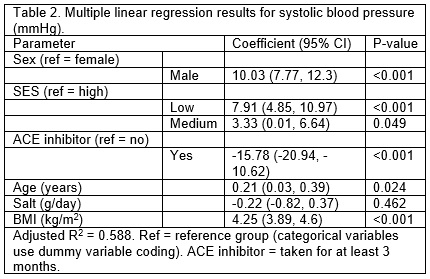
\includegraphics{C:/OneDrive - University of Leeds/Teaching/MSc IH/YCHI5045M/Teaching materials/Computer sessions/YCHI5045M practical sessions website/Images/Linear regression table.jpg}
\caption{Linear regression results table}
\end{figure}

\textbf{Example text interpreting the relationship between BMI and systolic blood pressure in terms of its statistical and practical importance}

There was a clear and precise, statistically significant relationship between BMI (kg/m²) and systolic blood pressure (mmHg) in the linear regression model, indicating that for every 1-unit increase in BMI there is a mean increase in systolic blood pressure of 4.25 mmHg (95\% CI: 3.89, 4.6) independent of all other independent variables. Given that the range of BMI in the study was 23, the relatively narrow confidence intervals for this relationship indicate that variation in BMI has the potential to have a very substantial impact on variation in systolic blood pressure in the target population, and given BMI is potentially variable by individuals and interventions this has clearly important clinical and practical implications. For example, this result suggests an increase in BMI of just 10 could potentially lead to an increase of between 39 mmHg (3.9 x 10) and 46 mmHg (4.6 x 10) in an individual's systolic blood pressure on average, implying this should be considered when developing treatment guidelines and public health programmes.

\textbf{Example text interpreting the relationship between sex and systolic blood pressure in terms of its statistical and practical importance}

There was a clear and precise, statistically significant relationship between sex (male/female) and systolic blood pressure (mmHg) in the linear regression model, indicating that compared to females males had systolic blood pressure values that were on average 10.03 mmHg (95\% CI: 7.77, 12.3) higher, independent of all other independent variables. Therefore, considering that the mean difference is likely to be between 7.77 mmHg and 12.3 mmHg this appears to be a potentially important clinical difference that should be considered when developing treatment guidelines and public health programmes (for example, by educating males on their higher risk of having higher systolic blood pressure).

\textbf{Example text discussing the key limitations of the study and the issues that must be considered when critically interpreting the results}

Care must be taken when interpreting the results because the study was an observational cross-sectional study with therefore very limited ability to make robust causal inferences, and because the validity and accuracy of the results depends on how well the study data and model have accurately captured the causal relationships of interest and all important confounding variables of those causal relationships, and on how much bias there was in the study.

\hypertarget{next-steps-optional-1}{%
\section{Next steps (optional)}\label{next-steps-optional-1}}

\begin{itemize}
\item
  If you have time why not run the sensitivity analysis for the extremely influential observations? Simply remove them from the dataset (go to the Data View and right click on their observation number on the left of the screen to highlight the relevant row, then select ``Clear''), re-run the model and compare the results to those above.
\item
  Confirm to yourself that an independent t-test is equivalent to a simple linear regression with one binary independent variable: using the ``SBP final data.sav'' dataset run an independent t-test analysing the difference/relationship between sex and systolic blood pressure, and then run a linear regression with systolic blood pressure as the outcome and sex as the sole independent variable. You should see that the coefficient estimate from the linear regression matches the mean difference estimate from the t-test, and the 95\% confidence intervals and p-values match as well. Underlying the independent t-test is a model that is equivalent to a simple linear regression!
\end{itemize}

\hypertarget{multiple-binary-logistic-regression}{%
\chapter{Multiple binary logistic regression}\label{multiple-binary-logistic-regression}}

\hypertarget{overview-14}{%
\section{Overview}\label{overview-14}}

Like multiple linear regression multiple binary logistic regression allows us to analyse the relationships between any number of continuous and/or categorical independent variables and an outcome, but unlike multiple linear regression the outcome in multiple binary logistic regression must be binary. Like with linear regression ``simple logistic regression'' may be a term used to refer to logistic regression with one independent variable only, while ``multiple linear regression'' refers to including more than one independent variable, but there's no qualitative difference, and we'll just refer to ``logistic regression'' from here on. Also, as touched on in the lecture there are different versions or extension of binary logistic regression like multinomial logistic regression for categorical outcomes with any number of category levels, but as these are more advanced we will not be looking at them further. Therefore, because ``binary logistic regression'' is far more commonly used/seen than any other form of logistic regression we'll just refer to it as logistic regression from here on, which is common practice (i.e.~if you see ``logistic regression'' in the literature you can assume it's referring to binary logistic regression).

You can actually analyse binary outcomes using linear regression, and you will sometimes see such analyses in the literature (sometimes called a ``linear probability model'') and you can often get reasonably useful (i.e.~reasonably accurate/unbiased) results. However, generally this is not recommended because of the often substantial disadvantages and problems with this approach. For example, the model predictions may range outside 0-1 (the only values your outcome can take in reality when viewed as a probability of the event occurring), and your inferences are likely to be biased because the assumptions of linear regression cannot be met in such a situation, producing biased confidence intervals and p-values. Although logistic regression is more complex mathematically the basic idea of creating a linear model (where the terms are additive) with numerical or categorical independent variables is the same, although the interpretation of the terms differs substantially.

\hypertarget{scenario-12}{%
\section{Scenario}\label{scenario-12}}

We will use almost exactly the same scenario as for the linear regression practical, using the SBP final dataset again. However, now we wish to understand the likely causes of variation in individuals' \emph{hypertension status} (rather than their systolic blood pressure), or more generally the likelihood of having hypertension, where we define hypertension as having a systolic blood pressure ≥140 mmHg, using the data collected in the SBP dataset. Refer to the ``The datasets'' section within the ``Introduction to SPSS'' section for full details if you need a full reminder, but briefly this dataset contains data on 556 individuals who were (hypothetically speaking!) sampled in a cross-sectional survey, and had data collected on their systolic blood pressure plus certain socio-demographic (age, sex, socio-economic status) and health characteristics (BMI, salt intake and ACE inhibitor usage).

\hypertarget{modelling-process}{%
\section{Modelling process}\label{modelling-process}}

We will use an almost identical modelling process to that used in the linear regression practical, loosely following a causal inference inspired approach, but in practice for simplicity building one model and interpreting all the independent variables causally. As discussed in the ``Overview with a focus on causal inference from observational data'' section in the ``Inferential analysis 5: multiple regression'' section, we will assume, based on existing theory/evidence and plausible, critical thinking, that all our measured independent variables are all likely causes of variation in individuals' hypertension status, which collectively simultaneously act as a sufficient adjustment set when interpreting each independent variable's relationship with the outcome causally. That is, we will just create one logistic regression model containing all the independent variables and assume that this model represents the same sufficient adjustment set for each independent variable (i.e.~when interpreting the effect of each independent variable causally we will assume all other variables in the model are confounders of that relationship that require adjusting for to obtain an unbiased estimate of the focal causal effect). In reality if we were doing this we should start by deciding which focal relationships of interest we were interested in, which may well not be all of our collected independent variables, and for each focal relationship of interest we should define a sufficient adjustment set which may well differ from the sufficient adjustment set of other focal relationships of interest. This would typically be a big and time consuming process requiring a lot of careful critical thought and research/subject matter knowledge.

\begin{itemize}
\tightlist
\item
  Load the ``SBP data final.sav'' dataset.
\end{itemize}

\hypertarget{step-1-explore-the-data-1}{%
\section{Step 1: explore the data}\label{step-1-explore-the-data-1}}

\href{https://youtu.be/uMGDhnJyl7I}{Video instructions: explore the data for a logistic regression}

\textbf{Written instructions: explore the data for a logistic regression}

The same basic reasoning applies to our data exploration process as with the linear regression modelling process, so refer back to the ``Step 1: explore the data'' section in the linear regression practical if you want a reminder of the theory/justification for the following data exploration process.

In practical terms though we would examine the distribution of each variable on its own using the same methods discussed in the linear modelling practical, but when examining the relationships between the outcome and each independent variable we would have to use different graphical approaches.

\hypertarget{numerical-independent-variables-1}{%
\subsection{Numerical independent variables}\label{numerical-independent-variables-1}}

Specifically, as we have a binary outcome when exploring the relationship between numerical independent variables and our binary outcome we have to use a form of barchart, where we first create a ``binned'' or grouped version of our numerical independent variable (i.e.~a new variable which takes a single value for a range of values of the original independent variable).

Let's see how to do this for bmi. First create the binned independent variable.

\begin{itemize}
\tightlist
\item
  From the main menu go: Transform \textgreater{} Visual Binning. Add bmi to the Variables to Bin: box and click Continue. At the top of the window that apppears look for the Name: fields and in the editable field called Binned Variable: give your new binned variable a name, e.g.~bmi\_bin. Then at the bottom right click on the Make Cutpoints\ldots{} button. In the middle of the tool window click the Equal Percentiles Based on Scanned Cases option and in the Intervals - fill in either field are click on the Number of Cutpoints: box and enter a suitable number of cutpoints. It's hard to know what is a suitable number but typically the more bins the better, as you can see relationships at a finer scale, but for more bins you need more data (sample size). For bmi let's choose 15, but you can always remake this variable with more/fewer bins as needed. Therefore, enter 15 in this box and then click Apply at the bottom. Then click the Make Labels button just below the Make Cutpoints\ldots{} button and then click OK. Click OK on the information box that appears.
\end{itemize}

Now we can plot the mean of our binary outcome, which is equivalent to the proportion/percentage, for every bin we've just created, using a type of barchart, although we'll use a ``histogram'' tool to create it.

\begin{itemize}
\tightlist
\item
  From the main menu go: Graphs \textgreater{} Chart Builder. If an information box appears saying ``Before you use this dialogue\ldots{}'' just click OK. Now in the Gallery tab at the middle left click on Histogram and then double click on the leftmost picture of a graph (Simple Histogram) to add it to the plot. Next drag the htn variable from the Variables: box onto the Y-Axis? dotted box on the chart image. Similarly, drag the bmi\_bin variable onto the X-Axis? box. Look to the right of the tool window at the Element Properties tab in the Statistics box. You should see a drop down menu under Statistic:. This should already read ``Mean'', but if not click on it and select mean. This tells SPSS to calculate the mean of the Y-axis variable, htn, for each value of the X-axis variable, which are now repeated when in each bin. Now just click OK.
\end{itemize}

What can you see?

What does the barchart of BMI vs hypertension show?

There appears to be a fairly linear increase in the proportion of individuals with hypertension as BMI values increase.

\hypertarget{categorical-independent-variables-1}{%
\subsection{Categorical independent variables}\label{categorical-independent-variables-1}}

For exploring the relationship between categorical independent variables and binary outcomes we can just use a normal barchart where the Y-axis is the proportion of the outcome in each category level on the X-axis. Let's see how to do this for sex:

\begin{itemize}
\tightlist
\item
  From the main menu go: Graphs \textgreater{} Chart Builder. If an information box appears saying ``Before you use this dialogue\ldots{}'' just click OK. Now in the Gallery tab at the middle left click on Bar and then double click on the top leftmost picture of a barchart (Simple Bar) to add it to the plot. Next drag the htn variable from the Variables: box onto the Y-Axis? dotted box on the chart image. Similarly, drag the sex variable onto the X-Axis? box. Look to the right of the tool window at the Element Properties tab in the Statistics box. You should see a drop down menu under Statistic:. This should already read ``Mean'', but if not click on it and select mean. This tells SPSS to calculate the mean of the Y-axis variable, htn, for each value of the X-axis variable, which are now repeated when in each bin. Now just click OK.
\end{itemize}

What can you see?

What does the barchart of sex vs hypertension show?

Men appear to have roughly twice the proportion of hypertension cases compared to women.

In a real analysis you would explore all bivariate relationships this way, but as with the linear regression practical feel free to move on once you are happy with the process.

\hypertarget{cell-frequencies}{%
\subsection{Cell frequencies}\label{cell-frequencies}}

Unlike with linear regression we have one more data exploration process that we must do. When looking at relationships for a logistic regression model an important issue to look out for is so-called ``sparse data'', which means we have small (or empty) ``cell sizes'', which really means few (or no) observations of one of the levels of our binary outcome (e.g.~either htn = yes or htn = no) in one or more levels of one or more categorical variables (e.g.~if say all men were classed as htn = yes). This is explained in more detail during the ``Additional potential problems'' section below, but briefly if there are zero observations of one outcome level within one or more independent categorical variable levels that will cause the model to fail. If there are just a few you may see very large biased coefficients and confidence intervals. How few is few? There's not set number, but \textless5 is often a cause for concern.

We can explore this issue using cross tabulations of the outcome variable against the categorical independent variables.

\begin{itemize}
\tightlist
\item
  Go: Analyze \textgreater{} Descriptive Statistics \textgreater{} Crosstabs. Add htn to the Row(s): box and sex, ses and ace to the Col(s): box then click OK.
\end{itemize}

This will give us three tables, one for each categorical variable. Look at each cross-tabulation cell to see the number of observations in that cell, i.e.~each possible combination of the independent categorical variable's level and the outcome's level, which for sex vs htn would include 1) male-yes, 2) male-no, 3) female-yes, and 4) female-no. What can you see?

What does the cross-tabulation show?

There appear to be reasonable numbers of observations of both levels of the outcome for all levels of sex and ses, but ACE = yes has only three htn = yes observations. See the ``Additional potential problems'' for more discussion of the possible problems this might cause.

\hypertarget{step-2-run-the-logistic-regression-model}{%
\section{Step 2: run the logistic regression model}\label{step-2-run-the-logistic-regression-model}}

\href{https://youtu.be/e1IHf2dX_5U}{Video instructions: run the logistic regression model}

\textbf{Written instructions: run the logistic regression model}

We will use SPSS's Generalized Linear Model tool to build our logistic regression model. The generalised linear modelling framework is a more comprehensive and coherent way of (mathematically) representing the full range of possible regression type models, of which linear regression and logistic regression are specific types. SPSS somewhat confusingly and redundantly also has a Binary Logistic tool under the Regression menu, which will also create a logistic regression model, but like the Linear (Regression) tool in the Regression menu it is also more restrictive because it won't accept categorical variables without us first converting them to separate dummy variables, and it also does not offer all the options available in the Generalized Linear Model tool.

\begin{itemize}
\item
  From the menu go: Analyze \textgreater{} Generalized Linear Models. This will open the Generalized Linear Models tool which has multiple tabs along the top of the window.
\item
  In the first tab Type of Model look for the ``Binary Response or Events/Trials Data'' set of options and select Binary logistic. This tells SPSS we want to create a logistic regression model from among the many other possible generalised linear models (note: linear regression is also a specific type of generalised linear model, and could be run from this tool via the ``Scale Response'' Linear option).
\item
  Then click on the Response tab and add the htn variable to the Dependent Variable: box. Then click on the Reference Category\ldots{} button and under ``Reference Category'' select First (lowest value), which sets the lowest value in the htn variable, 0, as the reference category (i.e.~htn = no as the reference category) and click Continue (without recoding the outcome variable by changing this option we could make our results refer to the likelihood of not having hypertension if this suited our needs better).
\item
  Then click on the Predictors tab and add the categorical variables sex, ses and ace into the Factors: box and the numerical variables age, salt and bmi into the Covariates: box.
\item
  Then click on the Model tab and highlight all the independent variables in the Factors and Covariates: box (click on the top one, hold down shift and then click on the bottom one). Then under the ``Build Term(s)'' options ensure the Type: is set to Main effects (this should be the default) and click the right facing arrow to add the variables into the Model: box.
\item
  We will ignore the Estimation tab and just accept its defaults (this is where you can alter how the model is estimated).
\item
  Next click on the Statistics tab and in the ``Print'' options tick the Include exponential parameter estimates box.
\item
  We will ignore the EM Means tab and just accept its defaults (this is where you can tell SPSS to calculate certain predicted outcomes given certain contrasts between categorical variable levels other than those displayed by default via dummy coding, i.e.~where each level is compared to a reference level).
\item
  Next click on the Save tab and tick the Cook's distance option to save a variable of the Cook's distance values for each observation in the dataset. We'll come back to this, but it provides a measure of influence of each observation on the values of the regression coefficients.
\item
  Finally click OK.
\end{itemize}

As with the linear regression practical, before interpreting the results we should check the assumptions of the model are not violated, and if they are make any necessary changes before re-running the model.

\hypertarget{step-3-check-the-assumptions-of-the-logistic-regression}{%
\section{Step 3: check the assumptions of the logistic regression}\label{step-3-check-the-assumptions-of-the-logistic-regression}}

Unlike with linear regression logistic regression has fewer assumptions and they are not all easily checked. Specifically, logistic regression no longer assumes linearity in the relationship between the independent variables and the outcome, nor does it assume normality or homoscedasticity in the residuals. However, it does have some assumptions as discussed below.

\textbf{1. Binary outcome}

Self-explanatory! However, note that we can code the variable either way around depending on whether we want our results in relation to the likelihood of observing a given ``event'' or the ``non-event''. For example, for our hypertension variable we could obtain results in relation to the likelihood of having hypertension or of not having hypertension if we coded the outcome as 1 = hypertension or 1 = not hypertension respectively, or equivalently we can use the relevant SPSS model building options as explained in the ``Step 2: create the logistic regression model'' section to change the reference level.

\textbf{2. Independent observations}

As with linear regression logistic regression assumes observations are independent of one another, which we can assume for our study data here as it came from a simple random (cross-sectional) sample. However, if our study design implies this is not the case then we need to either use a method that can cope with this (beyond the scope of this course) or modify our data.

The alternatives aren't exactly the same as for linear regression though. For longitudinal (multi-time point) data we can again use logistic regression if we just use data from one time point. However, unlike with linear regression we cannot calculate a change value between two time points and analyse that with logistic regression because outcomes of 0-0 and 1-1 at two time points will both give us the same change score, but mean very different things. Similarly if we have nested or clustered observations, such as patients within clinics, we cannot calculate summary outcome values for each cluster, such as means, and use logistic regression as the values will no longer be binary. We may however calculate the proportion of events per cluster and, assuming the assumptions are met, use linear regression to analyse this cluster-level summary (proportion) outcome. Like with linear regression there are multi-level logistic regression models that can explicitly model clustered (or multi-level) data.

\textbf{3. Linearity of relationships between the log-odds and numerical independent variables}

This is similar to the linear regression linearity assumption, but differs in a key way. With logistic regression the model estimates the predicted log-odds of the outcome rather than the actual value of the outcome (0/1), also called the logit transformation of the outcome, for each observation (e.g.~individual), given/conditional on the values of the independent variable(s) for that observation. The logistic regression model assumes that there is a linear relationship between any numerical independent variable(s) and the log-odds of the outcome variable. In theory we can test this by looking at the relationship between the residuals and the predicted/fitted values or numerical independent variables, but the resulting plots can be difficult to interpret usefully as you can still get curved patterns but due to the nature of logistic regression not have a model that has violated this assumption. See the following for more discussion:

\begin{itemize}
\item
  \url{https://stats.stackexchange.com/questions/121490/interpretation-of-plot-glm-model}
\item
  \url{https://stats.stackexchange.com/questions/45050/diagnostics-for-logistic-regression}
\end{itemize}

Hence, we won't produce such plots here and instead recommend that you think very carefully about the model you are building in terms of whether you have allowed for any strong/important non-linear relationships and/or interactions that evidence suggests may be present.

\hypertarget{step-4-consider-additional-problems}{%
\section{Step 4: consider additional problems}\label{step-4-consider-additional-problems}}

\textbf{1. Adequate sample size}

Although you should always consider your sample size when conducting any statistical analysis logistic regression requires more data than a hypothetically equivalent linear regression to achieve the same level of precision in its estimates, because there is less statistical information in an outcome than can only take two values. There are various rules of thumb. A common one is having at least 10 observations (e.g.~individuals) that have the \emph{least frequent outcome} (i.e.~that either have the event or do not have the event of interest, depending on whether having the event or not is more common in the sample) for each independent variable in your model. For example, if you have three independent variables and the overall proportion of your least frequent outcome, say not having hypertension, is 0.1, then you would need a minimum sample size of (10 x 3) / 0.1 = 300. All such rules are just rough guides, and it doesn't mean you can't build a model with less data, but they give you a good idea about the likely amount of data you need for decent precision. If you do have a much smaller sample size than these guides you'll typically find you have very wide confidence intervals for all your coefficients, making meaningful inference difficult, and it increases your chances of getting ``sparse data'' or ``complete separation'' (see next).

\textbf{2. No complete separation/sparse data}

Complete separation refers to the situation when one or more levels of one or more categorical variables levels have 100\% 1s or 100\% 0s observed for the outcome (e.g.~every male had ``hypertension'' or did not have ``hypertension''). In such a situation a standard logistic regression model cannot estimate the coefficient or standard error for that categorical variable level because there is no statistical variation in the outcome. The solutions are: 1) remove the entire variable, or 2) if possible recode the variable so that you ``collapse'' or merge two or more category levels together so that all levels have at least one (ideally more) of each possible observation (i.e.~a 1 or a 0), but the newly merged category levels must make logical sense for this to be a viable solution.

Sparse data refers to the situation where there are very few 1s or 0s observed in the outcome variable in one or more levels for one or more categorical variable levels (also referred to in this context as ``cells'', e.g.~the male and female cells for the variable sex). In such a situation with a standard logistic regression model the estimated coefficients and/or standard errors for that categorical variable level will often be very large and biased.

We checked the cell counts for each level of the outcome in the data exploration stage and found there were only 3 htn = yes observations in the ace = yes cell. There are rules of thumb for judging if a cell has sparse data, but really it's often easiest to just run the model and look at the results and if problems have occurred you will see extremely large (positive or negative) coefficient(s) and standard errors/confidence intervals. You can also check the cell counts for sex and ses if you wish, and you should do this for all categorical variables in a real data analysis situation, or you can move on as we know from earlier data exploration that they are fine.

\textbf{3. No serious multicollinearity}

Again if there is substantial multicollinearity between two or more independent variables this can cause serious problems with the model's ability to accurately estimate the results. As we are only looking at correlations between the independent variables when assessing multicollinearity we can just use the Linear Regression tool to calculate the VIF values again, but there is no need to repeat this process if you don't want to as the results will be identical to those from the linear regression practical VIF checking (because we have the same set of independent variables). Refer to the ``Step 4 consider additional possible issues'' section the linear regression practical for more details if needed.

\textbf{4. No extremely influential observations}

Lastly we again need to check that there are no observations that have an excessively influential effect on the results of the logistic regression model. We can again use a version of the Cook's distance statistic for logistic regression to check which observation(s), if removed, would change the coefficients substantially. When we ran the logistic regression via the Generalized Linear Model tool we told SPSS to calculate and save the Cook's distance values for each observation in a new variable, so as with the linear regression let's graph these against the observation ID. Graphs \textgreater{} Legacy Dialogues \textgreater{} Scatter/Dot and select the Simple Scatter option and click Define. Add the CooksDistance variable into the Y Axis: box and the id variable into the X Axis: box and click OK.

What do you see?

What do you see on the Cook's Distance plot?

There are two clearly excessively influential points. Interact with the graph to see which observations these are (double click, then click twice on one of the points to highlight it before right clicking and selecting ``Go to Case''). Unsurprisingly they are the same two observations that were highly influential for our linear regression: 478 and 520. We can again examine the values of the independent variables for each one again but the conclusion would be the same. Although they have independent variable values that mean the model predicts a very low likelihood of having hypertension we have no reason to think there are any errors in any of their data, and so we must keep them in our primary analysis, but best practice would be to perform a sensitivity analysis by removing them and exploring if our results and therefore our conclusions change substantially, and then transparently reporting this.

\hypertarget{step-5-understand-the-results-tables-and-extract-the-key-results-1}{%
\section{Step 5: understand the results tables and extract the key results}\label{step-5-understand-the-results-tables-and-extract-the-key-results-1}}

As we are now satisfied that the assumptions for our logistic regression model are not violated we can interpret the results. You can either scroll up in your output window or you may wish to re-run the model. By default, SPSS produces a whopping 8 tables, most of which are not that useful for us.

\begin{itemize}
\item
  ``Model information'' provides some basic information about our model.
\item
  ``Case Processing Summary'' provides information on how many observations were included and excluded from the model (all those with any missing outcome and/or independent variable data are automatically excluded).
\item
  The ``Categorical Variable Information'' and ``Continuous Variable Information'' tables provide descriptive information about all the categorical and continuous (also discrete numerical) variables included.
\item
  ``Goodness of Fit'' provides information about how well our model fits, or explains, the data. As you can see there are many measures of goodness of fit, and they are of little use to us (they are primarily useful when comparing the fit of different competing models).
\item
  The ``Omnibus Test'' provides a useful overall test of goodness of fit based on the likelihood ratio. This test compares the fit of our model to the fit of an ``intercept only'' model, i.e.~a logistic regression of the htn variable with no independent variables, just an intercept or overall mean. Clearly, we would hope that our model explains or fits the data much better than an intercept only model, otherwise this is an indication that our independent variables have very little ability to explain variation in the outcome and your model therefore tells you nothing about what influences the outcome. If the p-value (the ``Sig.'' column of the table) is statistically significant at the 5\% level this is usually taken as evidence that the full model has a substantially better fit than the intercept only model. This is commonly reported along with the coefficients.
\item
  The ``Test of Model Effects'' is analogous to an ANOVA table and tells us which variables (but not separate categorical variable levels) are ``statistically significant'', but nothing about their effect sizes or precision. It is therefore of arguably limited value.
\end{itemize}

Finally, we get to the key ``Parameter Estimates'' table, which provides us with very similar analogous information as the linear regression parameter estimates table.

\textbf{Parameter estimates table columns explained}

\textbf{Parameter}

\begin{itemize}
\tightlist
\item
  Again, each row is for a different ``parameter'' or ``logistic regression coefficient'', which means a separate term in the logistic regression model. For numerical variables this means one row per variable. However, because each level of a categorical variable is actually treated as a separate ``dummy variable'' (coefficient) as standard in a logistic regression model each categorical variable level has its own row.
\end{itemize}

\textbf{B}

\begin{itemize}
\item
  B stands for betas, because in the logistic regression model when represented mathematically the effect (or coefficient) of each variable is usually represented by the Greek letter beta. The betas are more commonly referred to as the parameter estimates or the (logistic regression) coefficients. They tell us the estimated direction (positive or negative) and size of effect each parameter (i.e.~variable) in the regression model has on the outcome variable. However, with logistic regression the model parameters as originally estimated by the model are on the log-odds scale. Therefore, for all numerical independent variables they represent the expected mean change in the log-odds of the outcome variable being 1 for every 1-unit increase in the independent variable. For categorical variables with the default dummy coding the coefficients represent the expected mean difference or change in the log-odds of the outcome variable being 1 between each level and the reference level (e.g.~male compared to female). Remember by default SPSS sets the category level coded with the highest value as the reference level, and the reference level always has a coefficient value of 0.
\item
  A note on the intercept. Here the intercept now represents the log-odds or odds (for Exp(B)) of the outcome variable being 1 when the values for all numerical independent variables are set to 0, and for the reference levels of all categorical variables. Again, this will often not have a useful interpretation and is often not reported in a logistic regression results table.
\end{itemize}

\textbf{Std. Error}

\begin{itemize}
\tightlist
\item
  These are the standard errors for each coefficient, which estimate the sampling variability of the coefficients in the wider population. This is used when calculating the 95\% confidence intervals and p-value.
\end{itemize}

\textbf{95\% Wald Confidence Interval (Lower and Upper)}

\begin{itemize}
\tightlist
\item
  These are the lower and upper 95\% confidence intervals for each coefficient based on the Wald method of calculation (essentially assuming a normal distribution).
\end{itemize}

\textbf{Hypothesis Test (Wald Chi-Square, df and Sig.)}

\begin{itemize}
\tightlist
\item
  This section of the table provides hypothesis tests for each coefficient based on the Wald chi-square statistic and the given degrees of freedom. The p-value is in the ``Sig.'' column, and is again a two-tailed p-value. Assuming the true value of the coefficient is 0, this p-value represents the probability of obtaining a coefficient at least as great as that observed (positively or negatively) due to sampling error alone.
\end{itemize}

\textbf{Exp(B)}

\begin{itemize}
\item
  These are the exponentiated coefficients, i.e.~eβ. Trying typical exp(x) into Google where x is one of the coefficients on the log-odds scale. You will see it is now the Exp(B) value. By exponentiating the coefficients, we can transform them from the log-odds scale the odds ratio scale, which allows for more easily and intuitive interpretation. Therefore, they now have the following interpretations. For numerical variables they represent the multiplicative change in the odds of the outcome variable being 1 for every 1-unit increase in the independent variable. For categorical variables they represent the multiplicative difference in the odds of the outcome variable being 1 for each level of the categorical variable compared to the reference level. By multiplicative we mean on the multiplicative scale, so an odds ratio of 2 means the odds are multiplied by 2 (i.e.~double) for every 1-unit increase in a numerical variable or compared to the reference level of a categorical variable. Similarly, an odds ratio of 0.5 means the odds are multiplied by 0.5 (i.e.~halve) for every 1-unit increase in a numerical variable or compared to the reference level of a categorical variable. Therefore, on the multiplicative scale the null or no effect value is 1.
\item
  A note on the intercept. Here the intercept now represents the odds (for Exp(B)) of the outcome variable being 1 when the values for all numerical independent variables are set to 0, and for the reference levels of all categorical variables. Again, this will often not have a useful interpretation and is often not reported in a logistic regression results table.
\end{itemize}

\textbf{95\% Wald Confidence Interval for Exp(B) (Lower and Upper)}

\begin{itemize}
\tightlist
\item
  These are the (Wald-based) 95\% confidence intervals for the exponentiated coefficients, i.e.~for the estimated odds ratios.
\end{itemize}

Note: typically, only the exponentiated coefficients (and their 95\% confidence intervals) are presented in the results from a logistic regression model, due to them being much easier and more intuitive (but still not that intuitive!) to interpret than those on the original log-odds scale.

\hypertarget{step-6-report-and-interpret-the-results-1}{%
\section{Step 6: report and interpret the results}\label{step-6-report-and-interpret-the-results-1}}

Let's see how we interpret some the results in the parameter estimates table. We will only look at the exponentiated coefficients, i.e.~the odds ratios regression coefficients, and their confidence intervals as they are more easily interpreted and, as explained above, only the odds ratio scale results are typically presented instead of the original scale log-odds results. We'll also keep things briefer than for the same linear regression sections as most of the concepts apply here in the same way, but we're just dealing with ratio measures of relationships rather than differences/increases/decreases.

\hypertarget{understanding-and-interpreting-odds-ratios}{%
\subsection{Understanding and interpreting odds ratios}\label{understanding-and-interpreting-odds-ratios}}

Odds ratios are just ratios, like risk ratios, but when interpreting their direction and size mistakes can be easily made. First of all, unlike linear regression coefficients which can range (in theory) from negative infinity to positive infinity, odds ratios can range (in theory) from 0 to positive infinity. Because they are ratios the null value or no relationship/no effect value is 1, not 0 like for linear regression coefficients. This is because ratios are the result of dividing two numbers, so if those numbers are the same then the result is 1, whereas with linear regression the coefficients are differences, where a difference of 0 represents no difference. Therefore, odds ratios \textless1 represent a negative relationship and odds ratios \textgreater1 represent a positive relationship.

As odds ratios are ratios they are on the ``multiplicative scale'', and they therefore represent factors by which one set of odds is multiplicatively related to another. For example, an odds ratio of 2 indicates that the odds of an outcome in the group of interest are 2 times the odds of the outcome occurring in the reference or comparison group. Take care though. It is not correct to say that an odds ratio of 2 indicates that the odds in the group of interest are 2 times \emph{higher} than the odds in the reference group. To talk about odds ratios in terms of the odds for the group of interest being relatively higher or lower than the odds for the reference group you should first convert the odds ratio to a percentage using the following formulae:

\begin{quote}
When the odds ratio is \textgreater1 you can calculate the \% increase in odds as:
\end{quote}

\begin{quote}
\textbf{(OR -- 1) x 100}
\end{quote}

\begin{quote}
For example, for an odds ratio of 4.2:
\end{quote}

\begin{quote}
\textbf{(4.2 -- 1) x 100 = 320\% increase in odds}
\end{quote}

\begin{quote}
When the odds ratio is \textless1 you can calculate the \% decrease in odds as:
\end{quote}

\begin{quote}
\textbf{(1 -- OR) x 100}
\end{quote}

\begin{quote}
For example, for an odds ratio of 0.45:
\end{quote}

\begin{quote}
\textbf{(1 -- 0.45) x 100 = 55\% decrease in odds}
\end{quote}

Note: you should of course refer to the upper and lower odds ratio confidence interval range when discussing results, and those values can be similarly transformed as above if desired.

Let's look at some examples to make this all clearer. We'll start with categorical independent variables as these are arguably easier to interpret than numerical independent variables.

\hypertarget{categorical-variables-2}{%
\subsection{Categorical variables}\label{categorical-variables-2}}

\begin{quote}
With the standard dummy coding of categorical variables (\url{https://stats.idre.ucla.edu/spss/faq/coding-systems-for-categorical-variables-in-regression-analysis-2/}) logistic regression coefficients for categorical variables represent the model-predicted mean (or more loosely the average) \emph{ratio} between the odds of the outcome for the categorical level (or group) of interest compared to the odds of the outcome for the reference or comparison level (or group), while holding the effect of all other independent variables constant, i.e.~they measure the mean independent relationship. The choice of which categorical level is set as the reference group is up to you.
\end{quote}

Let's take sex as an example. In the parameter estimates table the adjusted odds ratio and confidence interval for the category level male compared to the category level female was AOR = 3.53 (95\% CI: 2, 6.27). Note: AOR = adjusted odds ratio, because the odds ratio is adjusted for all other independent variables in the model. Therefore, the model predicts that males have odds of having hypertension that are 3.53 times the odds of having hypertension for females, or equivalently the model predicts that males have odds of having hypertension that are 254\% higher than the odds of having hypertension for females, while holding the effect of all other independent variables constant. The 95\% confidence intervals then tell us that the odds ratio for having hypertension in males compared to females is likely to be between 2 and 6.27 in the target population. Therefore, we have a reasonably accurate/precise estimate of this relationship. However, as always this is conditional on the level of bias in the results.

\hypertarget{numerical-variables-2}{%
\subsection{Numerical variables}\label{numerical-variables-2}}

Here are four \emph{equivalent} ways to interpret a logistic regression odds ratio coefficient for a numerical independent variable (i.e.~you can use any of these so it makes sense to use the one you are most comfortable with):

\begin{quote}
Logistic regression coefficients for numerical independent variables represent the model-predicted mean (or more loosely the average) \emph{ratio} between the odds of the outcome for a 1-unit increase in the independent variable compared to the odds of the outcome without a 1-unit increase in the independent variable, while holding the effect of all other independent variables constant, i.e.~they measure the mean independent relationship.
\end{quote}

\begin{quote}
Or you may find it easier to think in terms of the multiplicative change in the odds for every 1-unit increase in the independent variable: logistic regression coefficients for numerical independent variables represent the model-predicted mean (or more loosely the average) \emph{multiplicative change} in the odds of the outcome for every 1-unit increase in the independent variable, while holding the effect of all other independent variables constant.
\end{quote}

\begin{quote}
Or you may find it easier to think in terms of the number of times the odds change for every 1-unit increase in the independent variable: logistic regression coefficients for numerical independent variables represent the model-predicted mean (or more loosely the average) number of times the odds of the outcome change for every 1-unit increase in the independent variable, while holding the effect of all other independent variables constant. Therefore, for any given odds ratio ``OR'' regression coefficient for a numerical independent variable you can say that ``the model-predicts that the odds of the outcome change OR times for every 1-unit increase in the independent variable, while holding the effect of all other independent variables constant.''
\end{quote}

\begin{quote}
Or you can convert the odds ratio to a percentage change in the odds (i.e.~percentage increase or decrease in the odds) using the formulae above and interpret it in those terms: logistic regression coefficients for numerical independent variables represent the model-predicted mean (or more loosely the average) percentage change in the odds of the outcome for every 1-unit increase in the independent variable, while holding the effect of all other independent variables constant.
\end{quote}

I usually prefer to use either the third or final interpretation/wording.

Note: for all these equivalent interpretation the ratio/change/relationship does not depend on the value of the independent variable, i.e.~the same ratio/change/relationship is assumed to exist across the full range of values that the independent variable can take in the sample data, but it should not be considered to hold if you were considering values of the independent variable outside of the range of values seen in the sample data.

Let's take salt intake (in grams/day) as an example. From the parameter estimates table we can see the odds ratio for this numerical independent variable is AOR = 0.96 (95\% CI: 0.85, 1.14). Therefore, the model predicts that the odds of having hypertension change 0.96 times for every extra gram of salt consumed per day, while holding the effect of all other independent variables constant. Or equivalently the model predicts that the odds of having hypertension decrease by 4\% for every extra gram of salt consumed per day, while holding the effect of all other independent variables constant. The 95\% confidence intervals imply that the odds ratio in the target population is between 0.85 and 1.14, and therefore we cannot be confident whether the true relationship in the target population is positive or negative, although we can be confident that the true odds ratio is unlikely to be very large whether positively or negatively. As always though this is conditional on the level of bias in the results.

\hypertarget{practical-importance}{%
\subsection{Practical importance}\label{practical-importance}}

Similar considerations apply when trying to interpret the practical importance of the results of a logistic regression analysis of a study as those discussed for a linear regression. Therefore, see the discussion about interpreting the practical importance of numerical independent variables and categorical independent variables in the linear regression practical notes above (in particular see the ``Numerical variables'' section).

However, as shown in the lecture on logistic regression, it is also much more difficult to interpret the results of a logistic regression in terms of the real world importance for clinical/public health practice and policy etc than those from a linear regression for two reasons.

First, odds ratios are relative measures of a relationship and you cannot interpret their absolute impact without knowing what the odds (or probability/prevalence) of the outcome are in the reference group. Therefore, an odds ratio of 100 might not represent much of an absolute increase in the probability of occurrence of some event if that event is rare, while an odds ratio of 2 might represent a large absolute increase in the probability of occurrence of some event if that event is common. For example, if the probability of developing a rare cancer is 0.001\% then a risk factor that increased the odds of developing the cancer 100 times (i.e.~an odds ratio of 100) would only result in a probability of developing the cancer 0.1\%. While if the probability of developing a common cancer is 25\% then a risk factor that increased the odds of developing the cancer just 2 times (i.e.~an odds ratio of 2) would result in a probability of developing the cancer of 40\%.

Second, odds ratios are ratios of odds, and for most people odds are not as intuitive as probabilities of an outcome. However, we can use the following formula to approximate the relative risk (or risk ratio), which is arguably more easily interpreted as it's in terms of the probabilities of the outcome:

\begin{quote}
Approximate relative risk = adjusted or crude odds ratio / (1 − p0 + (p0 x adjusted orcrude odds ratio))
\end{quote}

As explained in the lecture the adjusted/crude odds ratio is the adjusted/crude odds ratio for the independent variable of interest (it will only be a crude estimate if the independent variable of interest is the only independent variable in the model), while p0 is the risk in the baseline/reference/control/comparison group. Also as explained in the lecture, in an observational study with multiple variables in a logistic regression model p0 will vary depending on both the value of the independent variable of interest and all other independent variables. Therefore, in such a situation we can try and estimate a range (lower and upper value) of plausible baseline risks to use in the calculation along with the range of adjusted odds ratios implied by the 95\% confidence interval of the adjusted odds ratio. We will not look not at this further here, but be aware of the challenges with interpreting results from logistic regression models in practice, and if you plan to use logistic regression (and indeed sophisticated analyses more generally) frequently in the future then the best advice is to learn how to do them in \emph{R} (free) or \emph{Stata} where you can then use their functions for estimating predicted probabilities of the outcome at different values of the independent variables, making it very easy to calculate risk ratios or even better risk differences along with the actual predicted probabilities, making for much more intuitive practical interpretation of your model results!

\hypertarget{non-significant-results-1}{%
\subsection{``Non-significant results''}\label{non-significant-results-1}}

The same advice applies when reporting and discussing non-significant results from a logistic regression as for a linear regression. Therefore, see the ``\,`Non-significant results'\,'' section in the linear regression practical session for details.

\hypertarget{regression-tables-1}{%
\subsection{Regression tables}\label{regression-tables-1}}

The same advice applies when reporting and presenting results from a logistic regression as for a linear regression in terms of presentation via a table. Therefore, see the ``Regression tables'' section in the linear regression practical session for details. However, an additional comment would that it is most common for logistic regression results table to just present the exponentiated regression coefficients, i.e.~the odds ratio scale regression coefficients, rather than the original log-odds scale regression coefficients, which are harder to usefully interpret. You should always make it explicit and clear though what form of results you are presenting. You can always include these in the same table or a separate table (e.g.~as supplementary materials) if you need to. Also, there are various pseudo-R²s for logistic regression, but they are often criticised for their less than ideal meaning and interpretability. Hence, unless required you do not need to present an ``equivalent'' R² value. However, it is usually recommended to present the likelihood ratio (chi-square) test result p-value, which compares your model to an intercept-only model, as this at least indicates whether your model explains more variation in the data than a simple intercept-only model.

\hypertarget{methods-1}{%
\subsection{Methods}\label{methods-1}}

As usual in a methods section you should clearly explain why you used a logistic regression analysis and exactly what you did, including how all the variables were coded/what units they were in, if you modified any variables, how you dealt with any missing data etc.

\hypertarget{exercise-multiple-logistic-regression}{%
\section{Exercise: multiple logistic regression}\label{exercise-multiple-logistic-regression}}

\begin{itemize}
\tightlist
\item
  In the YCHI5045M computer sessions materials ``Exercises'' folder open the ``Exercises.docx'' Word document and scroll down to \textbf{Multiple logistic regression: the causes of variation in hypertension status}. Then follow the instructions in the exercise.
\end{itemize}

\textbf{Example completed linear regression results table}

\begin{figure}
\centering
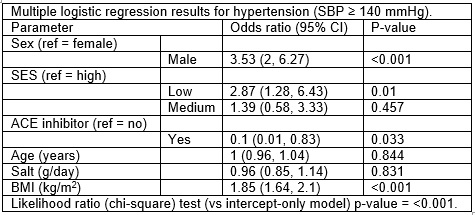
\includegraphics{C:/OneDrive - University of Leeds/Teaching/MSc IH/YCHI5045M/Teaching materials/Computer sessions/YCHI5045M practical sessions website/Images/Logistic regression table.jpg}
\caption{Logistic regression results table}
\end{figure}

\textbf{Example statistical and practical interpretation of the relationship between BMI and hypertension status}

The model-predicted that the odds of having hypertension increased by 85\% (95\% CI: 64\%, 110\%) for every 1-unit increase in BMI (kg/m²), while holding the effect of all other independent variables constant. Therefore, there was a clear, statistically significant, positive relationship between BMI and hypertension status.

\textbf{Example statistical and practical interpretation of the relationship between socio-economic status and hypertension status}

The model-predicted that, on average, the odds of having hypertension for individuals in the low socio-economic group were 187\% (95\% CI: 28\%, 543\%) higher than the odds of having hypertension for individuals in the high socio-economic group, while, on average, the odds of having hypertension for individuals in the medium socio-economic group were 38\% (95\% CI: -42\%, 233\%) higher than the odds of having hypertension for individuals in the high socio-economic group. \emph{Note: as the lower confidence interval was for an odds ratio \textless1 it represents a percentage reduction in the odds and so you must indicate this by adding a negative symbol. You wouldn't have to do this if both confidence intervals were reductions if you had verbally stated that the percentage changes were ``reduction'' or ``decreases'', as doing both could be confusing (a double negative).} Therefore, there was a clear, statistically significant, positive relationship between having low socio-economic status compared to high socio-economic status and the odds of having hypertension, but no clear (``statistically non-significant'') relationship between having medium socio-economic status compared to high socio-economic status and the odds of having hypertension.

\textbf{Example text discussing the key limitations of the study and the issues that must be considered when critically interpreting the results}

Care must be taken when interpreting the results because the study was an observational cross-sectional study with therefore very limited ability to make robust causal inferences, and because the validity and accuracy of the results depends on how well the study data and model have accurately captured the causal relationships of interest and all important confounding variables of those causal relationships, and on how much bias there was in the study.

\hypertarget{next-steps-optional-2}{%
\section{Next steps (optional)}\label{next-steps-optional-2}}

If you have time you can run a sensitivity analysis for the excessively influential points 478 and 520. Delete the htn values for these observations (which will exclude all their data from the model) and re-run the model.

What happens to the results?

Although there are some minor changes, with the largest being for the effect of taking an ACE inhibitor, it seems fair to say there are no substantial changes to the interpretation of the results. You can therefore have greater confidence in the robustness of the primary results.

\hypertarget{complex-surveydesign-analysis}{%
\chapter{Complex survey/design analysis}\label{complex-surveydesign-analysis}}

\hypertarget{overview-15}{%
\section{Overview}\label{overview-15}}

Complex survey analysis as it is commonly known is simply the analysis of complex survey data using appropriately modified methods. You may also see it referred to as complex sample analysis. Despite the common name of complex survey analysis complex survey data does not have to have come from a ``survey'', which doesn't actually define a study design, although most complex survey datasets will be surveys. More generally or technically speaking, complex survey data is any dataset (i.e.~sample) that has come from a probability sampling method that has any combination of the following three ``complex design features'', with all three often being present together:

\begin{enumerate}
\def\labelenumi{\arabic{enumi}.}
\item
  Stratification
\item
  Cluster or clustered sampling
\item
  Unequal probabilities of selection for sampling units
\end{enumerate}

Such data may have come from a single cross-sectional sample, multiple cross-sectional samples (i.e.~multiple samples across time of different sampling units), or be true longitudinal data (i.e.~multiple samples across time of the same sampling units).

This type of data is most commonly encountered/analysed in global health research when working with large-scale, typically national-scale, cross-sectional household surveys, such as the Demographic and Health Surveys (DHS: \url{https://dhsprogram.com/}), the Multiple Indicator Cluster Surveys (MICS: \url{https://mics.unicef.org/}), the WHO STEPwise Approach to surveillance Surveys (STEPS: \url{https://www.who.int/ncds/surveillance/steps/en/}), and many countries' own household surveys. This is because large-scale household surveys almost always use all three of these key complex survey features of stratification, cluster sampling, and unequal probabilities of selection of sampling units. The reason they do this is usually for both pragmatic, logistical, and statistical/research reasons. Specifically, stratified sampling is often employed to both allow strata (typically an administrative level such as the region, often further stratified into urban and rural areas) to be independently sampled to ensure that each strata has a sufficient sample size to allow inferences to be made at the strata-level. Cluster sampling is primarily employed to reduce the logistical costs of sampling across huge geographical areas. While stratification and the multi-stage cluster sampling methods employed result in unequal probabilities of selection for sampling units (typically individuals).

Standard methods of analysis, or more technically the maths underlying those methods, such as the independent t-test and linear regression, assume that the data being analysed come from a simple random sample. However, any of the complex survey features mentioned above result in a violation of that assumption, which if not adjusted for would result in either biased point estimates (e.g.~biased regression coefficients) and/or biased standard errors of those point estimates (i.e.~biased variance estimates), which means biased confidence intervals and p-values. More specifically, not adjusting for clustering typically results in falsely narrow confidence intervals/falsely small p-values, while not adjusting for stratification can mean the analysis ``misses out'' of the benefits of a stratified sample, which can reduce the overall variation in the outcome and produce more precise results for a given sample size. And not adjusting for unequal probabilities of selection of sampling units typically results in both biased/inaccurate point estimates of characteristics/relationships and falsely narrow confidence intervals/falsely small p-values. Therefore, it is critical that we account or adjust for any complex survey design features in our analyses to obtain unbiased results.

Luckily there are modifications to all commonly used analytical methods, including t-tests and regression models (i.e.~linear and logistic and others that we've not looked at). And also fortunately we don't have to worry about the underlying maths. With statistical software like SPSS primarily all we have to do is tell the software which variables code for, or identify, the different complex design features, and then select the appropriate complex survey design version of the analysis we want to do. Then we proceed with our analysis like we would if we were analysing data from a simple random sample, i.e.~using the processes outlined in the earlier practical sessions.

In any high quality complex survey dataset that used stratification, cluster sampling, and unequal probabilities of selection of sampling units in its sampling design, there will be a variable that indicates which strata each observation (sampling unit) comes from and a variable that indicates which cluster sampling unit each observation comes from. There will also be a third variable that contains the survey weights, which are used to adjust for the unequal probabilities of selection of sampling units.

\hypertarget{a-very-brief-description-of-survey-weights}{%
\section{A very brief description of survey weights}\label{a-very-brief-description-of-survey-weights}}

Sampling with unequal probabilities of selection of sampling units results in unrepresentative samples (i.e.~unrepresentative of the target population). This may occur when using stratified sampling with disproportionate strata, or when using a multi-stage cluster sampling approach. To obtain representative results we must therefore ``map'' the survey sample back onto the target population. To do this survey data producers calculate/produce sampling weights. In the analysis these weights upweight (or increase the contribution) of observations from sampling units that were undersampled compared to proportion of the target population that they represent, and they downweight (or decrease the contribution) of observations from sampling units that were oversampled compared to proportion of the target population that they represent. These weights are then usually combined with two other sets of weights. One that attempts to correct for any missing observations, and one that uses any pre-existing, recent, robust data on characteristics of the target population (such as a recent census) to adjust for any remaining lack of representativeness still reflected in the sample. Once all three types of weight are combined this results in a final or ultimate survey weight variable.

Therefore, once we've identified these three variables and ``told'' SPSS which variables they are we can analyse our data and largely forget/ignore the fact that we are doing a complex survey version of our chosen analysis. The type of results we get and their interpretation will, broadly speaking, not change apart from in a few areas that we will look at in this practical session.

\hypertarget{further-reading}{%
\section{Further reading}\label{further-reading}}

Unfortunately, the best and most beginner-friendly textbook on complex survey data analysis, which also included examples using SPSS (as well as other statistical software) is now no longer available from the library (it was previously available online via the library). This book is: Heeringa, S., West, B.T., Berglund, P.A. (2017). Applied Survey Data Analysis (2nd ed.). Boca Raton, FL, USA: CRC Press. If you do plan on conducting complex survey analyses in your later careers I would strongly recommend buying the book, as it's well worth it. The accompanying website also has lots of practice examples of analyses in SPSS and other statistical software. Unfortunately there are not any similar textbooks that I am aware of for complex survey analysis.

However, there is a nice overview/summary of the main issues around complex survey data analysis in the following paper, by one of the authors of the book I've just mentioned, which is freely available here:

\url{https://pubmed.ncbi.nlm.nih.gov/18956450/}

\hypertarget{preparing-for-complex-survey-data-analysis-a-checklist}{%
\section{Preparing for complex survey data analysis: a checklist}\label{preparing-for-complex-survey-data-analysis-a-checklist}}

The following is an excellent future reference checklist of steps to undertake when preparing to analyse complex survey data in a real analysis. It is taken from the Applied Survey Data Analysis textbook mentioned previously. For this practical we will assume we have carried out steps 1-3 and step 5 to save time, and some of the issues mentioned are beyond the scope of this introductory course/session, but if you were to do complex survey analysis for a real study or later in your career you should educate yourself enough to understand all these terms and the issues they refer to (e.g.~by buying and reading the recommended textbook).

\begin{enumerate}
\def\labelenumi{\arabic{enumi}.}
\item
  Review the documentation for the data set provided by the data producer, specifically focusing on sections discussing the development of the final survey weights and sampling error (standard error) estimation. Contact the data producer if any questions arise.
\item
  Identify the correct weight variable for the analysis, keeping in mind that many survey data sets include separate weights for different types of analyses. Perform simple descriptive analyses of the weight variable, noting the general distribution of the weights, whether the weights have been normalized, and whether there are missing or 0 weight values for some cases. Select a few key variables from the survey data set and compare weighted and unweighted estimates of descriptive parameters (e.g., means, proportions) for these variables to understand the effect the weights have.
\item
  Identify the variables in the data set containing the ``sampling error calculation codes'' that define the sampling error calculation model {[}JPH: these are just the variables defining the strata and clusters{]}. Examine how many clusters were selected from each sampling stratum (according to the sampling error calculation model), and whether particular clusters have small sample sizes. If only a single sampling error cluster is identified in a sampling stratum, contact the data producer or consult the documentation for the data set for guidance on recommended variance estimation methods. Determine whether replicate sampling weights are present if sampling error calculation codes are not available, and make sure that the statistical software is capable of accommodating replicate weights (Section 4.2.1).
\item
  Create a final analysis data set containing only the analysis variables of interest (including the survey weights, sampling error calculation variables, and case identifiers) {[}JPH: this is optional. It's nice to keep your dataset tidy and no bigger than necessary for speed and manageability, but it obviously doesn't affect the analysis in anyway{]}. Examine univariate and bivariate summaries for the key analysis variables to determine possible problems with missing data or unusual values on the individual variables.
\item
  Review the documentation provided by the data producer to understand the procedure (typically nonresponse adjustment) used to address unit nonresponse or nonresponse to a wave or phase of the survey data collection. Analyse the rates and patterns of item missing data for all variables that will be included in the analysis. Investigate the potential missing data mechanism by defining indicator variables flagging missing data for the analysis variables of interest. Use statistical tests (e.g., chi-square tests, two-sample t-tests) to see if there are any systematic differences between respondents providing complete responses and respondents failing to provide complete responses on important analysis variables (e.g., demographics). Choose an appropriate strategy for addressing missing data using the guidance provided in Section 4.4 and Chapter 12 {[}JPH: we will not look at missing data issues in this practical, but most high quality complex survey datasets, such as the DHS surveys, include weights that incorporate adjustments for missing data that, while not perfect by any means, go some way to addressing bias from missing data by simply including the weights in the analysis as you should be doing anyway{]}.
\item
  Define indicator variables for important analysis subclasses. Do not delete cases that are not a part of the primary analysis subclass. Assess a cross-tabulation of the stratum and cluster sampling error calculation codes for the subclass cases to identify the distribution of the subclass across the strata and clusters defined by the sampling error calculation model. Consult a survey statistician prior to analysis of subclasses that exhibit the ``mixed class'' characteristic illustrated in Figure 4.4. Make sure to employ appropriate software options for unconditional subclass analyses if using TSL for variance estimation {[}JPH: we will look at this issue in more detail later in this practical session{]}.
\end{enumerate}

\hypertarget{scenario-13}{%
\section{Scenario}\label{scenario-13}}

The dataset we will use here is one of the DHS's ``model datasets'', and as such it was produced by the DHS for practicing analysis of DHS survey data. It is therefore representative of the types of data and data features (e.g.~complex survey features) found in DHS surveys, but it doesn't contain any real data from any country. DHS surveys typically result in the production of a number of datasets, primarily a household-level dataset and datasets for women, men, and children, plus potentially others. You can read more about DHS datasets here: \url{https://dhsprogram.com/data/}

However, we will just use the ``individual recode'' dataset in the SPSS .sav format (DHS helpfully makes their datasets available in other formats too). This contains data from the female respondents of the survey, who consist of all members of a selected household who are aged 15-49. This dataset is included in the ``Datasets'' folder of the ``YCHI5045M computer practical files.zip'', and is called ``ZZIR62FL.SAV''. The ``odd'' naming is due to DHS's naming conventions, which you can read about here: \url{https://www.dhsprogram.com/data/File-Types-and-Names.cfm}

More specifically, we will use the dataset to answer the research question ``what factors affect the time women report it takes someone from their household to reach the household's source of drinking water?''

We will assume that our causal inference based model building process has led us to hypothesise that the most likely set of causal influences on the time household members take to reach the household's source of drinking water are:

\begin{itemize}
\item
  The household location (urban or rural)
\item
  The wealth level of the household
\item
  The age of the ``head of the household''
\end{itemize}

Of course this is just a simplified assumption to make things easier for learning purposes. Then like with our regression analyses, and unlike in a proper causal inference driven approach, we will make the simplifying assumption that we are interested in the relationship between each of these independent variables and the outcome variable of ``time household members take to reach the household's source of drinking water'', i.e.~we assume all these independent variables are likely causally related to the outcome, but that together these independent variables collectively form the sufficient adjustment set for each of the separate focal relationships. Therefore, like with our regression analyses to simplify things we will just create one model containing all these variables and interpret the results as though we had, to the best of our knowledge, adjusted for all likely sources of confounding for each focal relationship.

First of all though we will identify, explore, and edit as necessary the key complex design variables of the survey. We will then explore our independent and outcome variables, and then produce descriptive statistics to describe the sample's characteristics in terms of the variables measured, as would commonly be found in the ``Table 1'' of a paper. Then finally we will produce our analytical model results.

\begin{itemize}
\tightlist
\item
  Load the ``ZZIR62FL.sav'' SPSS dataset.
\end{itemize}

\hypertarget{step-1-prepare-and-explore-the-data}{%
\section{Step 1: prepare and explore the data}\label{step-1-prepare-and-explore-the-data}}

\href{https://youtu.be/6gUS7-JTTnk}{Video instructions: prepare and explore the data}

\textbf{Written instructions: prepare and explore the data}

\hypertarget{basic-variable-details}{%
\subsection{Basic variable details}\label{basic-variable-details}}

\begin{itemize}
\item
  V005 = Women's individual sample weight (6 decimals) - numerical
\item
  V021 = Primary sampling unit - nominal
\item
  V023 = Stratification used in sample design - nominal
\item
  V025 = Type of place of residence - nominal
\item
  V115 = Time to get to water source - numerical (minutes)
\item
  V152 = Age of household head - numerical (years)
\item
  V190 = Wealth index - ordinal
\end{itemize}

\hypertarget{prepare-and-explore-the-data}{%
\subsection{Prepare and explore the data}\label{prepare-and-explore-the-data}}

As per the checklist steps 1-3 for any complex survey analysis you must first thoroughly review the survey technical/methodological documentation to understand the design of the survey and sampling process, and to understand which variables contain the stratification, clustering, and weighting information, and to understand any modifications of those variables that are required. To save time we will assume we have done this, and that we have removed all variables from the dataset other than these design variables and the independent and outcome variables.

Therefore, open the ZZIR62FL.SAV dataset. If a window appears with a message starting ``IBM SPSS Statistics is running in Unicode encoding mode\ldots{}'' just click Yes. We can assume that from reading the relevant technical/methodological literature on this survey we have identified the relevant complex design variables and our variables of interest and removed all other variables from the dataset. The information on the complex design variables can be found in the ``DHS Guide to Statistics'' (\url{https://dhsprogram.com/data/Guide-to-DHS-Statistics/Analyzing_DHS_Data.htm}), but you should also review the survey specific literature (each DHS survey has a final report with specific methodological details relevant to that survey, along with a full copy of the questionnaire used that you should always review).

\hypertarget{explore-and-edit-the-complex-design-variables}{%
\subsubsection{Explore and edit the complex design variables}\label{explore-and-edit-the-complex-design-variables}}

Therefore, V005 identifies the survey weights, V021 identifies the clusters (often called primary sampling units as they are the first stage of a multi-stage cluster sample), and V023 identifies the strata. However, and this shows why you must read survey methodological literature carefully, all DHS weights are stored multiplied by 1,000,000. This is for very technical computer science related reasons about floating point errors that we don't need to go into here, but the point is that to use the weight variable we therefore need to first divide all values by 1,000,000.

To do this from the main menu go: Transform \textgreater{} Compute Variable. Then in the Target Variable: box give our new variable a suitable name, say ``survey\_weight'', and in the Numeric Expression: box enter the following:

\begin{quote}
V005 / 1000000
\end{quote}

Then click OK. You can now delete the old V005 variable if you wish.

Before we go any further let's rename the other variables for ease of reference. We'll use the following names:

\begin{itemize}
\item
  V021 = cluster
\item
  V023 = strata
\item
  V025 = location
\item
  V115 = time\_water
\item
  V152 = age\_hhh
\item
  V190 = wealth
\end{itemize}

And let's also change the variables cluster, strata, location, and wealth to the variable type nominal so SPSS treats them as categorical variables (as they use numerical coding SPSS automatically treats them as numerical variables unless told otherwise).

Now let's explore the complex design variables. For a quick overview of their descriptive statistics remember you can just right click on each variable in either the Data view or Variable View and click on Descriptive Statistics. However, you should first change the strata (V023) and cluster variables. As our strata and cluster variables are both categorical this is probably sufficient, but it's worth producing a histogram for the numerical survey\_weight variable to visualise its distribution. What do the descriptive statistics and histogram show you for the three complex design variables?

What do the descriptive statistics and histogram show you for the three complex design variables?

There are no missing values for any of the variables. The observations are typically evenly distributed across clusters, but much less evenly distributed across strata. However, there are no concerning issues, such as a single observation in a cluster or strata, that might indicate data errors. The histogram of the weights shows a strongly right-skewed distribution with some potentially concerning extremely high weight values. If this was a real analysis it would be worth looking into these more closely, but we'll assume they're all fine.

\hypertarget{explore-and-edit-the-data-variables}{%
\subsubsection{Explore and edit the data variables}\label{explore-and-edit-the-data-variables}}

Next let's explore each of the data variables in turn. Again for a quick univariate exploration we can just use the same process as we used to explore the complex design variables.

What do the descriptive statistics and histogram show you for the four data variables?

There are no missing values for location, and there is a \textasciitilde40\%:60\% split between urban and rural located households of the women surveyed. There are 13 missing values of our outcome variable time\_water, and a histogram indicates that the variable appears to have a strongly ``bimodal'' distribution with two distinct ``peaks'', but we'll come back this shortly. There are 6 missing values of age\_hhh, and a histogram indicates that the variable is fairly normally distributed. There are no missing values of wealth, and observations are evenly distributed across it's five levels. This is to be expected because in DHS surveys the numerical household wealth index is categorised into five wealth quintiles by evenly separating increasing values of the variable into five levels/groups.

So back to the outcome variable. This is a good example of why a careful data exploration is important prior to any analysis, and why understanding your survey data and methodological documentation is so important. You can access the questionnaire that the model dataset is based on here: \url{https://dhsprogram.com/pubs/pdf/DHSQ6/DHS6_Questionnaires_5Nov2012_DHSQ6.pdf}

Scroll down to question 104 ``How long does it take to go there, get water, and come back?'', which is where our variable comes from.

What can you see about the possible response values?

Respondents can provide the number of minutes it takes them to go and collect water and come back, but for those who don't know their response is coded as 998:, which is the second peak we see on the histogram. Therefore, the distribution is not bimodal at all, we're just not looking at only the true/non-missing values.

Therefore, let's just look at the distribution of non-missing values for our outcome. Instead of deleting all observations where the response was ``don't know'' to our question of interest we can tell SPSS to treat the value 998 as a missing value for this variable. In the Variable View for the time\_water row click on the cell under the column Missing and click on the box with three dots in that appears to the right of the cell. In the Missing Values box that appears click the Discrete missing values button and in the first box enter 998 and then click OK.

Now re-run the histogram and what do you see?

The distribution of values is clearly strongly right-skewed. Remember that linear regression assumes that the \emph{residuals} are approximately normally distributed not the raw values of the outcome, and therefore once we adjust for all our independent variables our model may be valid. However, with such strong right-skew it looks likely that we'll have to transform the outcome or use a different model (e.g.~a valid alternative would be to dichotomise the outcome, i.e.~convert it into a binary variable, and use a logistic regression, although that would throw away a lot of statistical information and result in cruder inferences). We shall see!

\hypertarget{explore-bivariate-relationships}{%
\subsubsection{Explore bivariate relationships}\label{explore-bivariate-relationships}}

Let's look at the relationships between our independent variables and our outcome to check for any clearly non-linear relationships. In a real analysis we would also want to check for the presence of strong interactions, ideally that we would expect from theory, but that is beyond the scope of this practical and course.

As previously for numerical independent variables we use scatter plots.

\begin{itemize}
\tightlist
\item
  From the menu go: Graphs \textgreater{} Legacy Dialogues \textgreater{} Scatter/Dot, then select the default top-left Simple scatter option and click Define. Then add age\_hhh and water\_time to the appropriate X Axis: and Y Axis: boxes respectively and click OK.
\end{itemize}

It's hard to see much of a relationship there, and certainly no clear non-linear relationship.

Then for the two categorical independent variables again we can use box plots.

\begin{itemize}
\tightlist
\item
  From the main menu go: Graphs \textgreater{} Legacy Dialogues \textgreater{} Boxplot, then select Simple and click Define. Add the water\_time variable into the Variable: box and location into the Category Axis: box and click OK.
\end{itemize}

It's also hard to see much of a clear relationship here, but the median time for urban looks slightly higher than the median time for rural, but clearly there's a lot of variation in both category levels. If you repeat the graph but for wealth what do you see? Again, personally I can't see any clear relationships here.

\hypertarget{step-2-create-the-spss-complex-samples-plan-file}{%
\section{Step 2: create the SPSS ``complex samples plan file''}\label{step-2-create-the-spss-complex-samples-plan-file}}

\href{https://youtu.be/UWYEU385pvM}{Video instructions: create the SPSS ``complex samples plan file''}

\textbf{Written instructions: create the SPSS ``complex samples plan file''}

As mentioned previously in order to undertake valid analysis of a complex design dataset we must first tell SPSS which variables code for the complex design features in our sample. We only need to do this once.

\begin{itemize}
\item
  To do this from the main menu go: Analyse \textgreater{} Complex Samples \textgreater{} Prepare for Analysis. Then with the Create a plan file button selected click Next. Then in the Save Data As window that opens we need to first create a complex samples plan file that SPSS can store the information in about which variables code for the complex design features. Therefore, navigate to a suitable folder and enter a suitable name for the plan into the File name: box, such as ``water\_survey'', and then click Save. You can now identify the complex design variables coding for the strata, clusters, and weights to SPSS. Note: if you are working with data that comes from a complex sample using few than all three of these design features you can of course just identify those.
\item
  In the Analysis Preparation Wizard simply add the strata variable into the Strata: box, the cluster variable into the Clusters: box, and the survey\_weight variable into the Sample Weight: box. You can then just click Finish, because the default options are that you can set on the next pages by clicking Next are suitable.
\end{itemize}

You have now created your sampling plan file which can be reused for any analysis of this dataset, and we can now run any analysis that can account for a complex design using this file and SPSS will adjust for the stratification, clustering and weights.

\hypertarget{step-3-describe-the-sample}{%
\section{Step 3: describe the sample}\label{step-3-describe-the-sample}}

\href{https://youtu.be/tCDLVDrBN-g}{Video instructions: describe the sample}

\textbf{Written instructions: describe the sample}

Note: if you feel you are short on time then skip this exercise and move onto the next exercise that focuses on producing the inferential results.

We will calculate the mean for water\_time and age\_hhh and the frequency and percentage for each category level of location and wealth. Let's start with the numerical independent variables.

\begin{itemize}
\item
  From the main menu go: Analyse \textgreater{} Complex Samples \textgreater{} Descriptives, then in the Complex Samples Plan for Descriptives Analysis tool just click Continue as the complex samples plan file will be automatically selected. If for any reason it is not click Browse and locate and select it before clicking Continue.
\item
  Now in the Complex Samples Descriptives tool add time\_water and age\_hhh to the Measures: box. Then click the Statistics button and ensure that the Mean button is ticked and click Continue. For some reason there is no option to calculate the standard deviation or median. The range isn't affected by the complex design features though so you could still calculate that using the standard tool.
\end{itemize}

You'll see that water\_time has a mean of 24.61 and age\_hhh has a mean of 45.48. These are both adjusted for the complex design features of the sample. To compare to an analysis ignoring these features right click on the water\_time variable and select the Descriptive Statistics option. You'll see that the mean for water\_time is 23.74 when you ignore the complex design features. In this instance it's not a big difference, but this is the affect of accounting for the weights variable.

Now let's calculate the frequency and percentage for each category level of location and wealth.

\begin{itemize}
\item
  From the main menu go: Analyse \textgreater{} Complex Samples \textgreater{} Frequencies, then in the Complex Samples Plan for Descriptives Analysis tool just click Continue as the complex samples plan file will be automatically selected. If for any reason it is not click Browse and locate and select it before clicking Continue.
\item
  Now in the Complex Samples for Frequencies Analysis tool add location and wealth to the Frequency Tables: box, then click the Statistics button and select the Population size, Table percent, and the Unweighted count tick boxes, and then click Continue and then OK.
\end{itemize}

The resulting tables are not helpfully laid out! The \textbf{Estimate} column gives the frequencies adjusted for the weights in the top half of the table and the corresponding percentages adjusted for the weights in the bottom half of the table. Then the \textbf{Unweighted count} gives the frequencies not adjusted for the weights in both the top and bottom halves of the table, i.e.~the values are just repeated for some unclear reason.

For both means and frequencies and percentages you would usually want to provide the weight-adjusted descriptive statistics because they reflect the target population that you are making inferences to, given that the unadjusted sample results will be, by the sampling design, not representative of that target population while the adjusted results aim to be.

\hypertarget{step-4-run-the-complex-design-adjusted-linear-regression-model}{%
\section{Step 4: run the complex design adjusted linear regression model}\label{step-4-run-the-complex-design-adjusted-linear-regression-model}}

\href{https://youtu.be/SIgR57AbJwA}{Video instructions: run the complex design adjusted linear regression model}

\textbf{Written instructions: run the complex design adjusted linear regression model}

We are now ready to produce our analytical inferential statistics via our linear regression model. Again we can just use our existing complex samples plan file to adjust for the complex design features using the appropriate complex design linear regression tool.

\begin{itemize}
\item
  From the main menu go: Analyse \textgreater{} Complex Samples \textgreater{} General Linear Model. Remember a general linear model is a synonym for a linear regression.
\item
  On the Complex Samples Plan for General Linear Model tool click Continue. Now add water\_time into the Dependent Variable: box, location and wealth into the Factors: box, and age\_hhh into the Covariates: box. By default just the main effects of each variable are included in the model so unless you want to specify interactions you can ignore the Model button.
\item
  Next click the Statistics button and in the Model Parameters area ensure the Estimate and Confidence interval boxes are ticked, along with the Model Fit and Sample design information boxes below. Then click Continue.
\item
  We can ignore the Hypothesis Tests button and the Estimated Means button, but click the Save button and in the Save Variables are ensure the Predicted Values and Residuals boxes are ticked then click Continue.
\item
  We can also ignore the Options box so just click OK.
\end{itemize}

\hypertarget{step-5-check-the-assumptions-of-the-complex-design-linear-regression-model}{%
\section{Step 5: check the assumptions of the complex design linear regression model}\label{step-5-check-the-assumptions-of-the-complex-design-linear-regression-model}}

However, as always before interpreting the results we should check the model's assumption are not violated. In particular, we should check that the residuals are approximately normally distributed and not heteroscedastic. To check the first of these just plot a histogram of the saved residual values (the variable should be called Residual).

What do you see?

The residuals are clearly strongly right-skewed!

Therefore, we can either try and transform the outcome or use an alternative analysis, such as a logistic regression after dichotomising the outcome. For now let's see how we would interpret the results assuming that the assumptions were not violated, and then we will leave it as an exercise for you to re-run the model with a transformed outcome to see if that solves things, and then interpret the back-transformed results.

Note: in a real analysis you should check all assumptions are not violated. Just follow the instructions in the ``Step 2: check the assumptions of the linear regression'' section in the linear regression practical for guidance, and use the Residuals and Predicted variables produced by the complex design adjusted linear regression we just ran accordingly.

\hypertarget{step-6-understand-the-results-tables}{%
\section{Step 6: understand the results tables}\label{step-6-understand-the-results-tables}}

After running the model we see four tables (scroll up from the residual histogram you should have just created and anything else you've done since running the model).

The \textbf{Sample Design Information} table tells us some important things about our sample and design. In particular, it tells us how many cases (in our case women) were missing or not missing from the analysis, i.e.~our effective sample size: these are the valid and invalid \textbf{N} values, as well as the total unweighted sample size (\textbf{Total N}). It also tells us the estimated size of the target population, but this is only valid if the weights are not ``normalised'' to have a mean of 1, which DHS weights areso you can ignore this. It also tells us the number of strata (\textbf{Strata}) and clusters (\textbf{Units}), which serves as a check if all strata and clusters were included in the analysis or if any were left out due to missing observations in those strata/clusters.

The \textbf{Model Summary} table tells us the R² value for the model, although frustratingly not the more robust and useful \emph{adjusted} R² value!

We can ignore the \textbf{Test of Model Effects} table as this is an ANOVA type table and not really useful.

Then we have our familar \textbf{Parameter Estimates} table where we get our key inferential results about the relationships between the independent variables and the outcome in the model. These are interpreted in exactly the same way as the linear regression coefficients from a linear regression that does not adjust for any complex design features. Therefore, refer back to the ``Step 6: report and interpret the results'' section of the linear regression practical, and in particular the sub-sections ``Numerical variables'' and ``Categorical variables'', for a reminder if needed.

\hypertarget{exercise-complex-design-adjusted-linear-regression}{%
\section{Exercise: complex design adjusted linear regression}\label{exercise-complex-design-adjusted-linear-regression}}

\begin{itemize}
\tightlist
\item
  In the YCHI5045M computer sessions materials ``Exercises'' folder open the ``Exercises.docx'' Word document and scroll down to \textbf{Complex design adjusted linear regression: the causes of variation in time taken to fetch water}. Then follow the instructions in the exercise.
\end{itemize}

\textbf{Example statistical interpretation of the relationship between household location, household wealth, and age of household head, and the time taken for household members to fetch water}

There was a clear, statistically significant relationship between household location and time taken for household members to fetch water, with women from households in location=1 reporting that it took household members a mean of 7.9 minutes (95\% CI: 1.5, 14) longer to fetch water than women from households in location=2. However, there was no clear relationship between household wealth or age of household head on the time taken by household members to fetch water. The R² value associated with the model was just 0.03, and therefore the model explained just 3\% of the variation in the time taken by household members to fetch water. Therefore, the model explained very little about what is likely to drive differences in the time taken by household members to fetch water. As always the accuracy of these inferences depend on the amount of bias in the study and analysis.

\textbf{Example statistical interpretation of the relationship between household location, household wealth, and age of household head, and the ln-transformed time taken for household members to fetch water}

Once the outcome was log-transformed the model residuals appeared very normally distributed, but there were no longer any clear relationships between any of the independent variables and the log-transformed outcome.

\textbf{Well done for getting to the end! If all of this seemed like very hard work that's because it is, but hopefully you feel like all your hard work has gained you some powerful new knowledge and skills. However, probably the most important lesson we hope you take away from this course is this: anyone can run complicated statistical analyses with modern statistical software, but it takes a lot of hard work, careful thought, and experience from continuous practice and learning, to make robust, valid, and meaningful statistical inferences. Hopefully you can also see that being able to do robust and useful statistical analyses is a hugely powerful skill to have.}

\textbf{We wish you all the best with the rest of your studies and in your future careers.}

  \bibliography{book.bib,packages.bib}

\end{document}
